\chapter{Introduction}
Over the past twenty years \emph{topological data analysis} has been found to be very useful in understanding scientific data. The primary tools of the field, persistent homology and mapper, have been used in a wide variety of applications, including image processing~\cite{cid-lbs-08}, material science~\cite{SW-measuring-shape}, and cosmology~\cite{cosmic-web}. Unlike traditional data analysis, in which one concerns itself with modeling physical phenomena from measurements on finite sets of samples, topological data analysis assumes that the input point cloud $X$ comes from an unknown underlying geometric space $Y$ embedded in some known larger ambient space $Z$. Topological data analysis then focuses on the recovery of the lost topology of $Y$ using information about $X$ and $Z$~\cite{c-tnd-09}. In this thesis we aim to make the primary tool for topological data analysis, persistent homology, computable for practitioners. To this end we investigate parallel algorithms for the computation of persistent homology. This implies providing a mechanism for decomposing a topological space, performing persistence computations on subspaces, and then gluing this information back together. For a topologist, this means exploiting the \emph{\mv principle}. The main contributions in this work are two new parallel algorithms, the first for computing homology via \mv{}, and the second which improves the running time of the algorithm and extends it to the persistent setting. We connect these procedures to \emph{spectral sequences}, a manual calculation tool used for computing algebraic structures by hand. To this end we also re-introduce persistent homology within the language of spectral sequences.

The structure of the thesis is as follows. First, we introduce general background material on algebraic topology and persistent homology. Second, to introduce spectral sequences, we will derive persistent homology using the spectral sequence of a filtration. Next, we will show how one can leverage the \emph{\mv spectral sequence}, to compute ordinary homology. We then provide a description of a parallel algorithm using the \mvb{} an analogous topological space. We take a brief digression to discuss the complexity of finding decompositions of a space which yield efficient parallel computation. Finally, we will show how to modify this construction to provide a parallel algorithm for persistence based on Mayer-Vietoris. Additionally we will show how one can derive upper bounds on the fill-in of these reduced matrices in terms of the quality of the cover. We will present experimental results which explore the efficacy of these techniques.

\section{Background}

 \begin{figure}
\centering
 \hspace{.5cm}
 \begin{tikzpicture}[scale=.25]
\begin{pgfonlayer}{ball}
      \foreach[count=\p] \x / \y in \data {
         \fill[gray!50,radius= .3 cm] (\x,\y) circle{};
	}
 \end{pgfonlayer}{ball}
	\foreach[count=\p] \x / \y in \data {
	 \node[draw, circle, scale=.25, fill=white](\p) at (\x, \y) {};
	 }
\end{tikzpicture}
 \hspace{.25cm}
\begin{tikzpicture}[scale=.25]
\begin{pgfonlayer}{ball}
      \foreach[count=\p] \x / \y in \data {
         \fill[gray!50,radius= .6 cm] (\x,\y) circle{};
	}
 \end{pgfonlayer}{ball}
	\foreach[count=\p] \x / \y in \data {
	 \node[draw, circle, scale=.25, fill=white](\p) at (\x, \y) {};
	 }
\end{tikzpicture}
 \hspace{.25cm}
\begin{tikzpicture}[scale=.25]
\begin{pgfonlayer}{ball}
      \foreach[count=\p] \x / \y in \data {
         \fill[gray!50,radius= 1 cm] (\x,\y) circle{};
	}
	\fill[gray!50,radius= 2.4 cm] (0,0) circle{};
 \end{pgfonlayer}{ball}
	\foreach[count=\p] \x / \y in \data {
	 \node[draw, circle, scale=.25, fill=white](\p) at (\x, \y) {};
	 }
\end{tikzpicture}
\caption{Model spaces at various scales}
\label{model-spaces}
\end{figure}

Suppose someone asked you describe the shape of the point cloud show in Figure~\ref{fig:point-cloud-annulus}. One might be inclined to propose that the point cloud looks quite disconnected. Indeed, the topology of a set of points in $\R^n$ is not all that interesting. Perhaps, however, if you were to squint your eyes, you might be inclined to describe the shape as something like an annulus. Persistence is a tool for modeling this phenomenon. As an example, for any \emph{metric space} $(X,d)$ and  $\epsilon > 0$ we can define a space: \[ M_\epsilon = \bigcup_{x \in X} B_{\epsilon}(x) \] where $B_{\epsilon}(x) = \{ y \mid d(x,y) < \epsilon\} $ is the \emph{ball of radius $\epsilon$ centered around x}. Notice that by varying the scale parameter $\epsilon$ one finds that the model space $M_\epsilon$ has different topologies. $M_\epsilon$ at various scales is shown in Figure~\ref{model-spaces}. The collection $\{M_\epsilon\}_\epsilon$ of spaces together with the inclusion maps between $M_\epsilon$ and $M_{\epsilon'}$ for any $\epsilon < \epsilon'$ is called a \emph{one parameter family} of spaces.   
 
Persistent topology concerns itself with capturing topological features which can be found at multiple scales of a parameterized family of spaces.
\begin{figure}
\centering
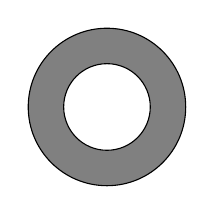
\begin{tikzpicture}[scale=.25]
  \filldraw[draw=black,fill=gray] (0,0) circle [radius=4];
      \filldraw[draw=black,fill=white] (0,0) circle [radius=2.2];
 \end{tikzpicture}      
 \hspace{.5cm}
\begin{tikzpicture}[scale=.25]
    \foreach[count=\p] \x / \y in \data { 
	\node[draw, circle, scale=.25, fill=white](\p) at (\x, \y) {};
    } 
 \end{tikzpicture}
 \caption{Point Cloud sampled from annulus}
\label{fig:point-cloud-annulus}
 \end{figure}
\section{Preliminaries}
We begin with a review of algebraic topology. We refer the reader to Hatcher for further background material in algebraic topology~\cite{hatcher}.
\subsection{Topological Spaces}
\begin{definition}{Topological Space.}
A \emph{topological space} on a set $X$ is a pair $(X,T)$ where $T$ is a subcollection of $P(X)$, containing $\emptyset$ and $X$, and is further closed under countable unions, and finite intersections. Elements of $T$ are referred to as \emph{open sets.}
\end{definition}
\begin{definition}{Closed Set.}
 The complement of an open set is a \emph{closed} set.
\end{definition}
\begin{figure}
\centering
\begin{tikzpicture}[y=0.80pt, x=0.8pt,yscale=1, inner sep=0pt, outer sep=0pt]
    %outer rectangle
    \path[draw=black,line join=round,miter limit=4.00,line width=2pt,rounded corners=0cm] (155,130) rectangle (555,226);
    %sphere
         \shade [ball color=afragreen]  (205,178) circle [radius=1cm];
  %line 1
    \path[draw=black,line join=miter,line cap=butt,miter limit=4, line width=2pt] (255,130) -- (255,226);    
    %torus
     \toruspicture{afragreen}
     %line 2 
     %mickey mouse
    \path[draw=black,line join=miter,line cap=butt,miter limit=4.00,line width=2pt] (355,130) -- (355,226);
    \mickeymouse{afragreen}
     %line 3 
     %mobius strip
    \path[draw=black,line join=miter,line cap=butt,miter limit=4.00,line width=2pt] (455,130) -- (455,226);
    \moebiustrip{afragreen}
  \end{tikzpicture}
\caption{Some topological spaces.}
\label{fig:example-ts}
\end{figure}
Some examples of topological spaces are, $D^n$ the unit $n$-disk in $\R^n$, $S^n$, the unit sphere in $R^{n+1}$, the mickey mouse $MM^2$, the torus $T^2$, and the mobius strip. The boundary of the $n$-disk is the $(n-1)$-ball. $\partial D^n = S^{n-1}$. These spaces are visualized in Figure~\ref{fig:example-ts}

\begin{definition}{Simplicial Complex}
A \emph{simplicial complex} is a collection $\K$ of finite sets called
\emph{simplices} such that if $\sigma \in \K$ and $\tau \subseteq \sigma$ then $\tau \in \K$. 
\end{definition}
In what follows, $\K$ is a simplicial complex, $\sigma \in \K$ and $\tau \subseteq \sigma$.
\begin{definition}{Dimension}
If $\card{\sigma} = k+1$, then $\sigma$ is a $k$-simplex, with \emph{dimension} $k$, denoted 
$\dim{\sigma} = k$. We say that $\K$ is \emph{$d$-dimensional} if 
$d = \max_{\sigma \in \K} \dim{\sigma}$.
\end{definition}
\begin{definition}{Faces \& Co-faces}
We say that $\tau$ is a \emph{face} of $\sigma$, its \emph{coface}. 
\end{definition}
\begin{definition}{Maximal Simplices}
A simplex is \emph{maximal} if it has no proper coface in $\K$. The set of maximal cells of a simplicial complex $\K$ is $\M(\K)$. 
\end{definition}
\begin{definition}{Subcomplexes}
Suppose $L \subseteq K$.  $L$ is a \emph{subcomplex} if it is a simplicial complex.
\end{definition}
\begin{definition}{Closure}
 The \emph{closure} of $L$ is $\Cl(L) = \{ \tau \mid \tau \subseteq \sigma \in L\}$ and it is a simplicial complex.
\end{definition}
\begin{definition}
The  \emph{$k$-skeleton} of a complex $\K$ is the set of all simplices
of dimension less than or equal to $k$. Note that the 1-skeleton of
any complex is a graph.
\end{definition}
\begin{definition}{Open Star}
The \emph{open star} of a simplex $\sigma$ is the set of simplices which have a face in $\sigma$, and denoted as $\operatorname{St}(\sigma)$. The star of a set $S$ of simplices is the union of the stars of those simplices.
\end{definition}
\begin{lemma}
$\operatorname{St}$ commutes with intersections.
\label{lem:st-inter}
\end{lemma}
A simplicial complex is a topological space, where the closed sets are specified by the closure of each simplex.
\begin{definition}{Subcomplexes of the standard $n$-simplex.}
Let $\Delta^n$ be the standard $n$-simplex~\cite{hatcher}. For any
\emph{indexing set} $J \subseteq [n]$, $\Delta^J$ is the $(\card{J}-1)$ 
dimensional face of $\Delta^n$  that is defined on $J$. In the abstract setting we may
identify $\Delta^n$ with the set $[n] = \{1, \ldots, n\}$ of natural numbers, and $\Delta^J$ with the set $J$.
\end{definition}
We can also define a simplicial complex geometrically. 
\begin{definition}{Geometric Simplex}
If $x_0, x_1, \ldots, x_k$ are $k+1$ affinely independent points in $\R^d$, then their convex hull is referred to as a \emph{geometric $k$-simplex}. Observe that any subset of affinely independent points is again affinely independent. 
\end{definition}
\begin{definition}{Geometric Simplicial Complex}
A collection $\K$ of geometric simplices, closed under the subset relation, is a \emph{geometric simplicial complex}. $\K$ together with the topology it inherits from $\R^d$ is referred to as the \emph{underlying topological space of $\K$} and is denoted $\card{\K}$. 
\end{definition}
\begin{definition}{Subdivision}
A simplicial complex $G$ is a \emph{subdivision} of a complex $\K$ if every simplex in $G$ is contained in a simplex in $K$. If $G$ and $\K$ are geometric we further require that $\card{G} = \card{K}$.
\end{definition}
\begin{definition}{Barycenter}
The \emph{barycenter} of a geometric simplex is the average of its vertices.
\end{definition}
\begin{definition}{Barycentric Subdivision}
Given a geometric simplicial complex $\K$, its \emph{barycentric subdivision} $G$ is defined as follows, First define $G_0$ to be the vertex set of $\K$. Then, define $G_i$ for $i > 0$ as follows: $G_i$ contains $G_{i-1}$ and additionally for each $i$-simplex $\sigma  \in \K$ we add its barycenter, and we introduce an $i$-simplex for each simplex $(i-1)$-simplex $\tau$ which bounds $\sigma$.
\end{definition}

A simplicial complex may be viewed as the result of gluing simplices of 
different dimensions along common faces. Other types of complexes are defined 
similarly using different types of \emph{cells}. Such \emph{cellular} complexes include \emph{cubical} complexes, \emph{simplicial sets}, $\Delta$-complexes, and \emph{CW-Complexes}, 
to name a few~\cite{ez-ssc-50,hatcher,kmm-ch-04,m-soat-68}. We end this section by introducing CW-Complexes.

\begin{definition}{CW-Complex}
 A finite dimensional CW-Complex $X$ is defined as the finite union $X = \bigcup_n X_n$, where $X_0$ is a given set of $0$-cells. One defines the $k$-cells $X_k$ inductively from $X_{k-1}$. To attach a $k$-cell $\sigma_\alpha$ construct an \emph{attaching map} $\phi_\alpha: S^{k-1} \rightarrow X_{k-1}$. We then define $X_k = X_{k-1} \sqcup D^k_\alpha / \sim$ where $x ~\sim \phi_\alpha(x)$ if $x \in \partial D^k_\alpha$. 
\end{definition}
In practice we only consider the class of  \emph{computable CW complexes} which are finite dimensional CW-complexes with computable attaching maps.
\begin{lemma}
Every simplicial complex is a CW-complex
\label{lem:simp-is-cw}
\end{lemma}
\begin{proof}
If $\K$ is a simplicial complex, it is identified with the CW-Complex which has a single $k$-cell per simplex $\sigma$, and an attaching map $\phi_\sigma$ whose image is $\partial(\sigma)$.  
\end{proof}
\begin{lemma}
The product of two CW-Complexes is a CW-Complex.
\label{lem:cw-complex-product}
\end{lemma}
\begin{proof}
If $X$ and $Y$ are CW-Complexes, then $X \times Y$ is a CW-Complex where the cells are the products of the cells in $X$ and $Y$ and the attaching maps are specified as the products of the attaching maps.
\end{proof}

\subsection{Maps, covers, and filtrations}
\begin{definition}{Continuous functions}
A map $f: X \rightarrow Y$ between topological spaces is \emph{continuous} if the inverse image of every (open/closed) set in $Y$ is ab (open/closed) set in $X$. 
\end{definition}
\begin{definition}{Homotopic Maps}
A pair of maps $f,g: X \rightarrow X$ are \emph{homotopic}, denoted $f \sim g$, if there is a continuous map $F: X \times [0,1] \rightarrow X$ with $F(x,0) = f(x)$ and $F(x,1) = g(x)$. 
\end{definition}
\begin{definition}{Homotopy Equivalence}
Two spaces are said to be \emph{homotopy equivalent}, denoted $X \simeq Y$, if there exists maps $f: X \rightarrow Y$ and $g: Y \rightarrow X$ such that $f \circ g \sim 1_Y$ and $g \circ f \sim 1_X$.
\end{definition}
\begin{definition}{Contractible}
A space $X$ is \emph{contractible} if it is homotopy equivalent to a point.
\end{definition}
\begin{definition}{Cover}
Given a simplicial complex $\K$, an \emph{open cover} of $\K$ is a collection of open sets $\{\C_i\}_i$, of $\K$ where $K = \bigcup_i \C_i$. Similarly, we call a cover closed if each element of the cover is a closed set.
\end{definition}
\begin{definition}{Nerve}
The \emph{nerve} $\N(\C)$ of a cover $\C$ is the simplicial complex on $[\card{\C}]$ whose $k$-simplices represent the non-trivial intersections of subsets of $\C$ of size $k+1$. The nerve may be regarded as a subcomplex of $\Delta^n$ and so we may denote its simplices by $\Delta^J$ where $J \subseteq [\card{\C}-1]$.
\end{definition}
Let $\K$ be any topological space, $\C$ be any cover of it, and $\N$ be the nerve of $\C$. 
\begin{lemma}
If every element of a finite closed cover $\C$, as well as all non-empty intersections of elements in $\C$, are contractible, then $\N$ is homotopy equivalent to $\K$.
\end{lemma}
\begin{proof}
See~\cite{hatcher}.
\end{proof}
Recall from the previous section that a sequence of spaces connected by continuous maps is referred to as a one-parameter family. Let $M = \{M_\epsilon\}$ be the one-parameter family defined in the previous section. Let $\C = \{\C_\epsilon\}$ be the collection of open sets in $\R^n$, defining every member of $M$. We may define another one-parameter family $\{ \N_\epsilon \}$ where $\N_\epsilon$ is the nerve of $\C_\epsilon$. Observe that whenever $\epsilon < \epsilon'$ there is an inclusion map: $\N_\epsilon \rightarrow \N_{\epsilon'}$.
We now redefine $N_{\epsilon}$ geometrically.
\begin{definition}{$\check{C}ech$ Complex}
The \emph{\check{C}ech}-Complex at scale $\epsilon$ is,
\[ C_\epsilon = \{ [ x_0, \ldots x_k] \mid \bigcap_i B_{\epsilon/2}(x_i)  \neq \emptyset \}. \]
\end{definition}
\begin{figure}
\centering
 \begin{tikzpicture}[scale=.5]
	\node[draw=none, fill=white] at (0, -5.5) {$\check{C}_{.6}$};
    \foreach[count=\p] \x / \y in \data {
	\begin{pgfonlayer}{ball}
        \fill[gray!50,radius= .6 cm] (\x,\y) circle{};
        \end{pgfonlayer}{ball}
	\node[draw, circle, scale=.25, fill=white](\p) at (\x, \y) {};
    } 
\begin{pgfonlayer}{edge} 
\draw (1) -- (6); 
\draw (1) -- (12); 
\draw (1) -- (19); 
\draw (1) -- (23); 
\draw (1) -- (26); 
\draw (1) -- (48); 
\draw (1) -- (50); 
\draw (1) -- (57); 
\draw (1) -- (68); 
\draw (1) -- (71); 
\draw (1) -- (96); 
\draw (1) -- (98); 
\draw (2) -- (8); 
\draw (2) -- (35); 
\draw (2) -- (47); 
\draw (2) -- (58); 
\draw (2) -- (64); 
\draw (2) -- (89); 
\draw (2) -- (97); 
\draw (3) -- (29); 
\draw (3) -- (39); 
\draw (3) -- (40); 
\draw (3) -- (51); 
\draw (3) -- (65); 
\draw (3) -- (73); 
\draw (3) -- (81); 
\draw (3) -- (91); 
\draw (3) -- (94); 
\draw (4) -- (59); 
\draw (4) -- (70); 
\draw (4) -- (85); 
\draw (4) -- (86); 
\draw (4) -- (88); 
\draw (4) -- (99); 
\draw (4) -- (102); 
\draw (5) -- (24); 
\draw (5) -- (54); 
\draw (5) -- (58); 
\draw (5) -- (63); 
\draw (5) -- (64); 
\draw (5) -- (100); 
\draw (6) -- (19); 
\draw (6) -- (26); 
\draw (6) -- (48); 
\draw (6) -- (57); 
\draw (6) -- (68); 
\draw (6) -- (71); 
\draw (6) -- (98); 
\draw (7) -- (15); 
\draw (7) -- (21); 
\draw (7) -- (39); 
\draw (7) -- (53); 
\draw (7) -- (81); 
\draw (8) -- (18); 
\draw (8) -- (24); 
\draw (8) -- (35); 
\draw (8) -- (54); 
\draw (8) -- (55); 
\draw (8) -- (63); 
\draw (8) -- (64); 
\draw (8) -- (89); 
\draw (9) -- (12); 
\draw (9) -- (23); 
\draw (9) -- (26); 
\draw (9) -- (28); 
\draw (9) -- (32); 
\draw (9) -- (50); 
\draw (9) -- (56); 
\draw (9) -- (67); 
\draw (9) -- (96); 
\draw (10) -- (29); 
\draw (10) -- (40); 
\draw (10) -- (49); 
\draw (10) -- (52); 
\draw (10) -- (65); 
\draw (10) -- (69); 
\draw (10) -- (77); 
\draw (10) -- (78); 
\draw (10) -- (80); 
\draw (10) -- (83); 
\draw (11) -- (13); 
\draw (11) -- (20); 
\draw (11) -- (33); 
\draw (11) -- (41); 
\draw (11) -- (44); 
\draw (11) -- (45); 
\draw (11) -- (46); 
\draw (11) -- (72); 
\draw (11) -- (90); 
\draw (11) -- (93); 
\draw (11) -- (95); 
\draw (12) -- (23); 
\draw (12) -- (25); 
\draw (12) -- (26); 
\draw (12) -- (28); 
\draw (12) -- (32); 
\draw (12) -- (50); 
\draw (12) -- (67); 
\draw (12) -- (68); 
\draw (12) -- (87); 
\draw (12) -- (96); 
\draw (12) -- (98); 
\draw (13) -- (20); 
\draw (13) -- (44); 
\draw (13) -- (61); 
\draw (13) -- (72); 
\draw (13) -- (82); 
\draw (13) -- (90); 
\draw (13) -- (95); 
\draw (14) -- (30); 
\draw (14) -- (31); 
\draw (14) -- (34); 
\draw (14) -- (43); 
\draw (14) -- (55); 
\draw (14) -- (60); 
\draw (14) -- (75); 
\draw (14) -- (76); 
\draw (14) -- (84); 
\draw (14) -- (92); 
\draw (15) -- (21); 
\draw (15) -- (39); 
\draw (15) -- (51); 
\draw (15) -- (53); 
\draw (15) -- (65); 
\draw (15) -- (73); 
\draw (15) -- (81); 
\draw (16) -- (17); 
\draw (16) -- (19); 
\draw (16) -- (38); 
\draw (16) -- (57); 
\draw (16) -- (62); 
\draw (16) -- (79); 
\draw (17) -- (22); 
\draw (17) -- (38); 
\draw (17) -- (57); 
\draw (17) -- (62); 
\draw (17) -- (74); 
\draw (17) -- (79); 
\draw (18) -- (35); 
\draw (18) -- (54); 
\draw (18) -- (55); 
\draw (18) -- (63); 
\draw (18) -- (64); 
\draw (18) -- (76); 
\draw (18) -- (89); 
\draw (19) -- (48); 
\draw (19) -- (57); 
\draw (19) -- (71); 
\draw (19) -- (79); 
\draw (20) -- (41); 
\draw (20) -- (44); 
\draw (20) -- (45); 
\draw (20) -- (46); 
\draw (20) -- (72); 
\draw (20) -- (82); 
\draw (20) -- (90); 
\draw (20) -- (93); 
\draw (20) -- (95); 
\draw (21) -- (39); 
\draw (21) -- (53); 
\draw (21) -- (81); 
\draw (21) -- (91); 
\draw (21) -- (94); 
\draw (21) -- (100); 
\draw (22) -- (70); 
\draw (22) -- (74); 
\draw (22) -- (85); 
\draw (22) -- (88); 
\draw (22) -- (99); 
\draw (23) -- (26); 
\draw (23) -- (28); 
\draw (23) -- (32); 
\draw (23) -- (50); 
\draw (23) -- (56); 
\draw (23) -- (67); 
\draw (23) -- (68); 
\draw (23) -- (87); 
\draw (23) -- (96); 
\draw (23) -- (98); 
\draw (24) -- (54); 
\draw (24) -- (58); 
\draw (24) -- (63); 
\draw (24) -- (64); 
\draw (25) -- (28); 
\draw (25) -- (32); 
\draw (25) -- (66); 
\draw (25) -- (67); 
\draw (25) -- (68); 
\draw (25) -- (87); 
\draw (25) -- (96); 
\draw (25) -- (98); 
\draw (26) -- (32); 
\draw (26) -- (50); 
\draw (26) -- (67); 
\draw (26) -- (68); 
\draw (26) -- (96); 
\draw (26) -- (98); 
\draw (27) -- (36); 
\draw (27) -- (37); 
\draw (27) -- (56); 
\draw (27) -- (101); 
\draw (28) -- (32); 
\draw (28) -- (37); 
\draw (28) -- (56); 
\draw (28) -- (66); 
\draw (28) -- (67); 
\draw (28) -- (87); 
\draw (28) -- (96); 
\draw (28) -- (101); 
\draw (29) -- (40); 
\draw (29) -- (51); 
\draw (29) -- (52); 
\draw (29) -- (65); 
\draw (29) -- (73); 
\draw (29) -- (77); 
\draw (29) -- (78); 
\draw (29) -- (80); 
\draw (29) -- (83); 
\draw (30) -- (31); 
\draw (30) -- (34); 
\draw (30) -- (43); 
\draw (30) -- (55); 
\draw (30) -- (60); 
\draw (30) -- (75); 
\draw (30) -- (76); 
\draw (30) -- (84); 
\draw (30) -- (92); 
\draw (31) -- (43); 
\draw (31) -- (55); 
\draw (31) -- (60); 
\draw (31) -- (75); 
\draw (31) -- (76); 
\draw (31) -- (84); 
\draw (31) -- (92); 
\draw (32) -- (50); 
\draw (32) -- (56); 
\draw (32) -- (67); 
\draw (32) -- (68); 
\draw (32) -- (87); 
\draw (32) -- (96); 
\draw (32) -- (98); 
\draw (33) -- (41); 
\draw (33) -- (46); 
\draw (33) -- (86); 
\draw (33) -- (93); 
\draw (34) -- (36); 
\draw (34) -- (37); 
\draw (34) -- (43); 
\draw (34) -- (60); 
\draw (34) -- (66); 
\draw (34) -- (75); 
\draw (34) -- (84); 
\draw (34) -- (92); 
\draw (35) -- (47); 
\draw (35) -- (55); 
\draw (35) -- (64); 
\draw (35) -- (76); 
\draw (35) -- (89); 
\draw (36) -- (37); 
\draw (36) -- (66); 
\draw (36) -- (84); 
\draw (36) -- (101); 
\draw (37) -- (56); 
\draw (37) -- (66); 
\draw (37) -- (101); 
\draw (38) -- (62); 
\draw (38) -- (74); 
\draw (39) -- (73); 
\draw (39) -- (81); 
\draw (39) -- (91); 
\draw (39) -- (94); 
\draw (40) -- (42); 
\draw (40) -- (49); 
\draw (40) -- (52); 
\draw (40) -- (73); 
\draw (40) -- (77); 
\draw (40) -- (78); 
\draw (40) -- (80); 
\draw (40) -- (83); 
\draw (41) -- (44); 
\draw (41) -- (45); 
\draw (41) -- (46); 
\draw (41) -- (72); 
\draw (41) -- (90); 
\draw (41) -- (93); 
\draw (41) -- (95); 
\draw (41) -- (102); 
\draw (42) -- (44); 
\draw (42) -- (49); 
\draw (42) -- (61); 
\draw (42) -- (69); 
\draw (42) -- (77); 
\draw (42) -- (78); 
\draw (42) -- (80); 
\draw (42) -- (82); 
\draw (42) -- (90); 
\draw (42) -- (95); 
\draw (43) -- (60); 
\draw (43) -- (75); 
\draw (43) -- (76); 
\draw (43) -- (84); 
\draw (43) -- (92); 
\draw (44) -- (45); 
\draw (44) -- (46); 
\draw (44) -- (49); 
\draw (44) -- (72); 
\draw (44) -- (82); 
\draw (44) -- (90); 
\draw (44) -- (93); 
\draw (44) -- (95); 
\draw (45) -- (46); 
\draw (45) -- (72); 
\draw (45) -- (82); 
\draw (45) -- (90); 
\draw (45) -- (93); 
\draw (45) -- (95); 
\draw (45) -- (102); 
\draw (46) -- (72); 
\draw (46) -- (90); 
\draw (46) -- (93); 
\draw (46) -- (95); 
\draw (46) -- (102); 
\draw (47) -- (55); 
\draw (47) -- (60); 
\draw (47) -- (89); 
\draw (48) -- (57); 
\draw (48) -- (68); 
\draw (48) -- (71); 
\draw (48) -- (79); 
\draw (48) -- (96); 
\draw (48) -- (98); 
\draw (49) -- (61); 
\draw (49) -- (69); 
\draw (49) -- (77); 
\draw (49) -- (78); 
\draw (49) -- (80); 
\draw (49) -- (82); 
\draw (49) -- (83); 
\draw (49) -- (90); 
\draw (49) -- (95); 
\draw (50) -- (67); 
\draw (50) -- (68); 
\draw (50) -- (96); 
\draw (50) -- (98); 
\draw (51) -- (52); 
\draw (51) -- (65); 
\draw (51) -- (73); 
\draw (52) -- (65); 
\draw (52) -- (73); 
\draw (52) -- (77); 
\draw (52) -- (78); 
\draw (52) -- (80); 
\draw (52) -- (83); 
\draw (53) -- (81); 
\draw (53) -- (100); 
\draw (54) -- (63); 
\draw (54) -- (64); 
\draw (55) -- (60); 
\draw (55) -- (75); 
\draw (55) -- (76); 
\draw (55) -- (89); 
\draw (55) -- (92); 
\draw (56) -- (67); 
\draw (56) -- (101); 
\draw (57) -- (71); 
\draw (57) -- (79); 
\draw (58) -- (64); 
\draw (58) -- (97); 
\draw (58) -- (100); 
\draw (59) -- (70); 
\draw (59) -- (85); 
\draw (59) -- (86); 
\draw (59) -- (88); 
\draw (59) -- (99); 
\draw (60) -- (75); 
\draw (60) -- (76); 
\draw (60) -- (84); 
\draw (60) -- (92); 
\draw (61) -- (69); 
\draw (61) -- (77); 
\draw (61) -- (78); 
\draw (61) -- (80); 
\draw (61) -- (82); 
\draw (61) -- (90); 
\draw (61) -- (95); 
\draw (62) -- (74); 
\draw (62) -- (79); 
\draw (63) -- (64); 
\draw (64) -- (89); 
\draw (65) -- (73); 
\draw (65) -- (83); 
\draw (66) -- (87); 
\draw (67) -- (68); 
\draw (67) -- (87); 
\draw (67) -- (96); 
\draw (67) -- (98); 
\draw (68) -- (71); 
\draw (68) -- (87); 
\draw (68) -- (96); 
\draw (68) -- (98); 
\draw (69) -- (77); 
\draw (69) -- (78); 
\draw (69) -- (80); 
\draw (69) -- (82); 
\draw (69) -- (83); 
\draw (69) -- (95); 
\draw (70) -- (74); 
\draw (70) -- (85); 
\draw (70) -- (88); 
\draw (70) -- (99); 
\draw (71) -- (79); 
\draw (71) -- (98); 
\draw (72) -- (82); 
\draw (72) -- (90); 
\draw (72) -- (93); 
\draw (72) -- (95); 
\draw (73) -- (81); 
\draw (73) -- (91); 
\draw (73) -- (94); 
\draw (74) -- (85); 
\draw (74) -- (88); 
\draw (75) -- (76); 
\draw (75) -- (84); 
\draw (75) -- (92); 
\draw (76) -- (84); 
\draw (76) -- (89); 
\draw (76) -- (92); 
\draw (77) -- (78); 
\draw (77) -- (80); 
\draw (77) -- (82); 
\draw (77) -- (83); 
\draw (78) -- (80); 
\draw (78) -- (83); 
\draw (80) -- (82); 
\draw (80) -- (83); 
\draw (81) -- (91); 
\draw (81) -- (94); 
\draw (82) -- (90); 
\draw (82) -- (93); 
\draw (82) -- (95); 
\draw (84) -- (92); 
\draw (85) -- (86); 
\draw (85) -- (88); 
\draw (85) -- (99); 
\draw (86) -- (99); 
\draw (87) -- (96); 
\draw (87) -- (98); 
\draw (88) -- (99); 
\draw (89) -- (92); 
\draw (90) -- (93); 
\draw (90) -- (95); 
\draw (91) -- (94); 
\draw (91) -- (97); 
\draw (93) -- (95); 
\draw (93) -- (102); 
\draw (96) -- (98); 
\end{pgfonlayer}{edge} 
\begin{pgfonlayer}{triangle} 
\fill[complex_triangle] (1.center) -- (19.center) -- (6.center) -- cycle; 
\fill[complex_triangle] (1.center) -- (26.center) -- (6.center) -- cycle; 
\fill[complex_triangle] (48.center) -- (1.center) -- (6.center) -- cycle; 
\fill[complex_triangle] (1.center) -- (6.center) -- (57.center) -- cycle; 
\fill[complex_triangle] (1.center) -- (68.center) -- (6.center) -- cycle; 
\fill[complex_triangle] (1.center) -- (6.center) -- (71.center) -- cycle; 
\fill[complex_triangle] (1.center) -- (98.center) -- (6.center) -- cycle; 
\fill[complex_triangle] (1.center) -- (12.center) -- (23.center) -- cycle; 
\fill[complex_triangle] (1.center) -- (26.center) -- (12.center) -- cycle; 
\fill[complex_triangle] (1.center) -- (50.center) -- (12.center) -- cycle; 
\fill[complex_triangle] (68.center) -- (1.center) -- (12.center) -- cycle; 
\fill[complex_triangle] (96.center) -- (1.center) -- (12.center) -- cycle; 
\fill[complex_triangle] (1.center) -- (98.center) -- (12.center) -- cycle; 
\fill[complex_triangle] (48.center) -- (1.center) -- (19.center) -- cycle; 
\fill[complex_triangle] (1.center) -- (19.center) -- (57.center) -- cycle; 
\fill[complex_triangle] (1.center) -- (19.center) -- (71.center) -- cycle; 
\fill[complex_triangle] (1.center) -- (26.center) -- (23.center) -- cycle; 
\fill[complex_triangle] (1.center) -- (50.center) -- (23.center) -- cycle; 
\fill[complex_triangle] (1.center) -- (68.center) -- (23.center) -- cycle; 
\fill[complex_triangle] (96.center) -- (1.center) -- (23.center) -- cycle; 
\fill[complex_triangle] (1.center) -- (98.center) -- (23.center) -- cycle; 
\fill[complex_triangle] (1.center) -- (26.center) -- (50.center) -- cycle; 
\fill[complex_triangle] (1.center) -- (26.center) -- (68.center) -- cycle; 
\fill[complex_triangle] (96.center) -- (1.center) -- (26.center) -- cycle; 
\fill[complex_triangle] (1.center) -- (26.center) -- (98.center) -- cycle; 
\fill[complex_triangle] (48.center) -- (1.center) -- (57.center) -- cycle; 
\fill[complex_triangle] (48.center) -- (1.center) -- (68.center) -- cycle; 
\fill[complex_triangle] (48.center) -- (1.center) -- (71.center) -- cycle; 
\fill[complex_triangle] (48.center) -- (1.center) -- (96.center) -- cycle; 
\fill[complex_triangle] (48.center) -- (1.center) -- (98.center) -- cycle; 
\fill[complex_triangle] (1.center) -- (50.center) -- (68.center) -- cycle; 
\fill[complex_triangle] (96.center) -- (1.center) -- (50.center) -- cycle; 
\fill[complex_triangle] (1.center) -- (50.center) -- (98.center) -- cycle; 
\fill[complex_triangle] (1.center) -- (71.center) -- (57.center) -- cycle; 
\fill[complex_triangle] (1.center) -- (68.center) -- (71.center) -- cycle; 
\fill[complex_triangle] (96.center) -- (1.center) -- (68.center) -- cycle; 
\fill[complex_triangle] (1.center) -- (98.center) -- (68.center) -- cycle; 
\fill[complex_triangle] (1.center) -- (98.center) -- (71.center) -- cycle; 
\fill[complex_triangle] (96.center) -- (1.center) -- (98.center) -- cycle; 
\fill[complex_triangle] (8.center) -- (2.center) -- (35.center) -- cycle; 
\fill[complex_triangle] (8.center) -- (64.center) -- (2.center) -- cycle; 
\fill[complex_triangle] (8.center) -- (89.center) -- (2.center) -- cycle; 
\fill[complex_triangle] (2.center) -- (35.center) -- (47.center) -- cycle; 
\fill[complex_triangle] (64.center) -- (2.center) -- (35.center) -- cycle; 
\fill[complex_triangle] (89.center) -- (2.center) -- (35.center) -- cycle; 
\fill[complex_triangle] (89.center) -- (2.center) -- (47.center) -- cycle; 
\fill[complex_triangle] (64.center) -- (2.center) -- (58.center) -- cycle; 
\fill[complex_triangle] (97.center) -- (2.center) -- (58.center) -- cycle; 
\fill[complex_triangle] (64.center) -- (89.center) -- (2.center) -- cycle; 
\fill[complex_triangle] (40.center) -- (3.center) -- (29.center) -- cycle; 
\fill[complex_triangle] (51.center) -- (3.center) -- (29.center) -- cycle; 
\fill[complex_triangle] (65.center) -- (3.center) -- (29.center) -- cycle; 
\fill[complex_triangle] (73.center) -- (3.center) -- (29.center) -- cycle; 
\fill[complex_triangle] (73.center) -- (3.center) -- (39.center) -- cycle; 
\fill[complex_triangle] (81.center) -- (3.center) -- (39.center) -- cycle; 
\fill[complex_triangle] (91.center) -- (3.center) -- (39.center) -- cycle; 
\fill[complex_triangle] (3.center) -- (94.center) -- (39.center) -- cycle; 
\fill[complex_triangle] (40.center) -- (73.center) -- (3.center) -- cycle; 
\fill[complex_triangle] (51.center) -- (3.center) -- (65.center) -- cycle; 
\fill[complex_triangle] (51.center) -- (3.center) -- (73.center) -- cycle; 
\fill[complex_triangle] (65.center) -- (3.center) -- (73.center) -- cycle; 
\fill[complex_triangle] (73.center) -- (3.center) -- (81.center) -- cycle; 
\fill[complex_triangle] (73.center) -- (91.center) -- (3.center) -- cycle; 
\fill[complex_triangle] (73.center) -- (3.center) -- (94.center) -- cycle; 
\fill[complex_triangle] (81.center) -- (91.center) -- (3.center) -- cycle; 
\fill[complex_triangle] (81.center) -- (3.center) -- (94.center) -- cycle; 
\fill[complex_triangle] (91.center) -- (3.center) -- (94.center) -- cycle; 
\fill[complex_triangle] (59.center) -- (4.center) -- (70.center) -- cycle; 
\fill[complex_triangle] (59.center) -- (4.center) -- (85.center) -- cycle; 
\fill[complex_triangle] (59.center) -- (4.center) -- (86.center) -- cycle; 
\fill[complex_triangle] (88.center) -- (59.center) -- (4.center) -- cycle; 
\fill[complex_triangle] (99.center) -- (59.center) -- (4.center) -- cycle; 
\fill[complex_triangle] (4.center) -- (85.center) -- (70.center) -- cycle; 
\fill[complex_triangle] (88.center) -- (4.center) -- (70.center) -- cycle; 
\fill[complex_triangle] (99.center) -- (4.center) -- (70.center) -- cycle; 
\fill[complex_triangle] (4.center) -- (85.center) -- (86.center) -- cycle; 
\fill[complex_triangle] (88.center) -- (4.center) -- (85.center) -- cycle; 
\fill[complex_triangle] (99.center) -- (4.center) -- (85.center) -- cycle; 
\fill[complex_triangle] (99.center) -- (4.center) -- (86.center) -- cycle; 
\fill[complex_triangle] (88.center) -- (99.center) -- (4.center) -- cycle; 
\fill[complex_triangle] (24.center) -- (5.center) -- (54.center) -- cycle; 
\fill[complex_triangle] (24.center) -- (58.center) -- (5.center) -- cycle; 
\fill[complex_triangle] (24.center) -- (5.center) -- (63.center) -- cycle; 
\fill[complex_triangle] (24.center) -- (64.center) -- (5.center) -- cycle; 
\fill[complex_triangle] (5.center) -- (54.center) -- (63.center) -- cycle; 
\fill[complex_triangle] (64.center) -- (5.center) -- (54.center) -- cycle; 
\fill[complex_triangle] (64.center) -- (58.center) -- (5.center) -- cycle; 
\fill[complex_triangle] (58.center) -- (100.center) -- (5.center) -- cycle; 
\fill[complex_triangle] (64.center) -- (5.center) -- (63.center) -- cycle; 
\fill[complex_triangle] (48.center) -- (19.center) -- (6.center) -- cycle; 
\fill[complex_triangle] (57.center) -- (19.center) -- (6.center) -- cycle; 
\fill[complex_triangle] (19.center) -- (6.center) -- (71.center) -- cycle; 
\fill[complex_triangle] (26.center) -- (68.center) -- (6.center) -- cycle; 
\fill[complex_triangle] (26.center) -- (98.center) -- (6.center) -- cycle; 
\fill[complex_triangle] (48.center) -- (57.center) -- (6.center) -- cycle; 
\fill[complex_triangle] (48.center) -- (68.center) -- (6.center) -- cycle; 
\fill[complex_triangle] (48.center) -- (6.center) -- (71.center) -- cycle; 
\fill[complex_triangle] (48.center) -- (98.center) -- (6.center) -- cycle; 
\fill[complex_triangle] (57.center) -- (6.center) -- (71.center) -- cycle; 
\fill[complex_triangle] (68.center) -- (6.center) -- (71.center) -- cycle; 
\fill[complex_triangle] (98.center) -- (68.center) -- (6.center) -- cycle; 
\fill[complex_triangle] (98.center) -- (6.center) -- (71.center) -- cycle; 
\fill[complex_triangle] (15.center) -- (21.center) -- (7.center) -- cycle; 
\fill[complex_triangle] (39.center) -- (15.center) -- (7.center) -- cycle; 
\fill[complex_triangle] (15.center) -- (53.center) -- (7.center) -- cycle; 
\fill[complex_triangle] (81.center) -- (15.center) -- (7.center) -- cycle; 
\fill[complex_triangle] (39.center) -- (21.center) -- (7.center) -- cycle; 
\fill[complex_triangle] (53.center) -- (21.center) -- (7.center) -- cycle; 
\fill[complex_triangle] (81.center) -- (21.center) -- (7.center) -- cycle; 
\fill[complex_triangle] (81.center) -- (39.center) -- (7.center) -- cycle; 
\fill[complex_triangle] (81.center) -- (53.center) -- (7.center) -- cycle; 
\fill[complex_triangle] (8.center) -- (18.center) -- (35.center) -- cycle; 
\fill[complex_triangle] (8.center) -- (18.center) -- (54.center) -- cycle; 
\fill[complex_triangle] (8.center) -- (18.center) -- (55.center) -- cycle; 
\fill[complex_triangle] (8.center) -- (18.center) -- (63.center) -- cycle; 
\fill[complex_triangle] (8.center) -- (64.center) -- (18.center) -- cycle; 
\fill[complex_triangle] (8.center) -- (89.center) -- (18.center) -- cycle; 
\fill[complex_triangle] (8.center) -- (24.center) -- (54.center) -- cycle; 
\fill[complex_triangle] (8.center) -- (24.center) -- (63.center) -- cycle; 
\fill[complex_triangle] (8.center) -- (24.center) -- (64.center) -- cycle; 
\fill[complex_triangle] (8.center) -- (35.center) -- (55.center) -- cycle; 
\fill[complex_triangle] (8.center) -- (64.center) -- (35.center) -- cycle; 
\fill[complex_triangle] (8.center) -- (89.center) -- (35.center) -- cycle; 
\fill[complex_triangle] (8.center) -- (54.center) -- (63.center) -- cycle; 
\fill[complex_triangle] (8.center) -- (64.center) -- (54.center) -- cycle; 
\fill[complex_triangle] (8.center) -- (89.center) -- (55.center) -- cycle; 
\fill[complex_triangle] (8.center) -- (64.center) -- (63.center) -- cycle; 
\fill[complex_triangle] (8.center) -- (64.center) -- (89.center) -- cycle; 
\fill[complex_triangle] (9.center) -- (12.center) -- (23.center) -- cycle; 
\fill[complex_triangle] (9.center) -- (26.center) -- (12.center) -- cycle; 
\fill[complex_triangle] (9.center) -- (12.center) -- (28.center) -- cycle; 
\fill[complex_triangle] (32.center) -- (9.center) -- (12.center) -- cycle; 
\fill[complex_triangle] (9.center) -- (50.center) -- (12.center) -- cycle; 
\fill[complex_triangle] (9.center) -- (67.center) -- (12.center) -- cycle; 
\fill[complex_triangle] (96.center) -- (9.center) -- (12.center) -- cycle; 
\fill[complex_triangle] (9.center) -- (26.center) -- (23.center) -- cycle; 
\fill[complex_triangle] (9.center) -- (28.center) -- (23.center) -- cycle; 
\fill[complex_triangle] (32.center) -- (9.center) -- (23.center) -- cycle; 
\fill[complex_triangle] (9.center) -- (50.center) -- (23.center) -- cycle; 
\fill[complex_triangle] (56.center) -- (9.center) -- (23.center) -- cycle; 
\fill[complex_triangle] (9.center) -- (67.center) -- (23.center) -- cycle; 
\fill[complex_triangle] (96.center) -- (9.center) -- (23.center) -- cycle; 
\fill[complex_triangle] (32.center) -- (9.center) -- (26.center) -- cycle; 
\fill[complex_triangle] (9.center) -- (26.center) -- (50.center) -- cycle; 
\fill[complex_triangle] (9.center) -- (26.center) -- (67.center) -- cycle; 
\fill[complex_triangle] (96.center) -- (9.center) -- (26.center) -- cycle; 
\fill[complex_triangle] (32.center) -- (9.center) -- (28.center) -- cycle; 
\fill[complex_triangle] (56.center) -- (9.center) -- (28.center) -- cycle; 
\fill[complex_triangle] (9.center) -- (67.center) -- (28.center) -- cycle; 
\fill[complex_triangle] (96.center) -- (9.center) -- (28.center) -- cycle; 
\fill[complex_triangle] (32.center) -- (9.center) -- (50.center) -- cycle; 
\fill[complex_triangle] (32.center) -- (9.center) -- (56.center) -- cycle; 
\fill[complex_triangle] (32.center) -- (9.center) -- (67.center) -- cycle; 
\fill[complex_triangle] (32.center) -- (9.center) -- (96.center) -- cycle; 
\fill[complex_triangle] (9.center) -- (50.center) -- (67.center) -- cycle; 
\fill[complex_triangle] (96.center) -- (9.center) -- (50.center) -- cycle; 
\fill[complex_triangle] (56.center) -- (9.center) -- (67.center) -- cycle; 
\fill[complex_triangle] (96.center) -- (9.center) -- (67.center) -- cycle; 
\fill[complex_triangle] (40.center) -- (10.center) -- (29.center) -- cycle; 
\fill[complex_triangle] (10.center) -- (52.center) -- (29.center) -- cycle; 
\fill[complex_triangle] (65.center) -- (10.center) -- (29.center) -- cycle; 
\fill[complex_triangle] (10.center) -- (29.center) -- (77.center) -- cycle; 
\fill[complex_triangle] (10.center) -- (29.center) -- (78.center) -- cycle; 
\fill[complex_triangle] (80.center) -- (10.center) -- (29.center) -- cycle; 
\fill[complex_triangle] (10.center) -- (83.center) -- (29.center) -- cycle; 
\fill[complex_triangle] (40.center) -- (49.center) -- (10.center) -- cycle; 
\fill[complex_triangle] (40.center) -- (10.center) -- (52.center) -- cycle; 
\fill[complex_triangle] (40.center) -- (10.center) -- (77.center) -- cycle; 
\fill[complex_triangle] (40.center) -- (10.center) -- (78.center) -- cycle; 
\fill[complex_triangle] (40.center) -- (80.center) -- (10.center) -- cycle; 
\fill[complex_triangle] (40.center) -- (10.center) -- (83.center) -- cycle; 
\fill[complex_triangle] (49.center) -- (10.center) -- (69.center) -- cycle; 
\fill[complex_triangle] (49.center) -- (10.center) -- (77.center) -- cycle; 
\fill[complex_triangle] (49.center) -- (10.center) -- (78.center) -- cycle; 
\fill[complex_triangle] (80.center) -- (49.center) -- (10.center) -- cycle; 
\fill[complex_triangle] (49.center) -- (10.center) -- (83.center) -- cycle; 
\fill[complex_triangle] (65.center) -- (10.center) -- (52.center) -- cycle; 
\fill[complex_triangle] (10.center) -- (52.center) -- (77.center) -- cycle; 
\fill[complex_triangle] (10.center) -- (52.center) -- (78.center) -- cycle; 
\fill[complex_triangle] (80.center) -- (10.center) -- (52.center) -- cycle; 
\fill[complex_triangle] (10.center) -- (83.center) -- (52.center) -- cycle; 
\fill[complex_triangle] (65.center) -- (10.center) -- (83.center) -- cycle; 
\fill[complex_triangle] (10.center) -- (69.center) -- (77.center) -- cycle; 
\fill[complex_triangle] (10.center) -- (69.center) -- (78.center) -- cycle; 
\fill[complex_triangle] (80.center) -- (10.center) -- (69.center) -- cycle; 
\fill[complex_triangle] (10.center) -- (83.center) -- (69.center) -- cycle; 
\fill[complex_triangle] (10.center) -- (77.center) -- (78.center) -- cycle; 
\fill[complex_triangle] (80.center) -- (10.center) -- (77.center) -- cycle; 
\fill[complex_triangle] (10.center) -- (83.center) -- (77.center) -- cycle; 
\fill[complex_triangle] (80.center) -- (10.center) -- (78.center) -- cycle; 
\fill[complex_triangle] (10.center) -- (83.center) -- (78.center) -- cycle; 
\fill[complex_triangle] (80.center) -- (10.center) -- (83.center) -- cycle; 
\fill[complex_triangle] (11.center) -- (20.center) -- (13.center) -- cycle; 
\fill[complex_triangle] (11.center) -- (44.center) -- (13.center) -- cycle; 
\fill[complex_triangle] (72.center) -- (11.center) -- (13.center) -- cycle; 
\fill[complex_triangle] (90.center) -- (11.center) -- (13.center) -- cycle; 
\fill[complex_triangle] (11.center) -- (13.center) -- (95.center) -- cycle; 
\fill[complex_triangle] (41.center) -- (11.center) -- (20.center) -- cycle; 
\fill[complex_triangle] (44.center) -- (11.center) -- (20.center) -- cycle; 
\fill[complex_triangle] (11.center) -- (20.center) -- (45.center) -- cycle; 
\fill[complex_triangle] (11.center) -- (20.center) -- (46.center) -- cycle; 
\fill[complex_triangle] (72.center) -- (11.center) -- (20.center) -- cycle; 
\fill[complex_triangle] (90.center) -- (11.center) -- (20.center) -- cycle; 
\fill[complex_triangle] (11.center) -- (20.center) -- (93.center) -- cycle; 
\fill[complex_triangle] (11.center) -- (20.center) -- (95.center) -- cycle; 
\fill[complex_triangle] (33.center) -- (11.center) -- (41.center) -- cycle; 
\fill[complex_triangle] (33.center) -- (11.center) -- (46.center) -- cycle; 
\fill[complex_triangle] (33.center) -- (11.center) -- (93.center) -- cycle; 
\fill[complex_triangle] (41.center) -- (11.center) -- (44.center) -- cycle; 
\fill[complex_triangle] (41.center) -- (11.center) -- (45.center) -- cycle; 
\fill[complex_triangle] (41.center) -- (11.center) -- (46.center) -- cycle; 
\fill[complex_triangle] (72.center) -- (41.center) -- (11.center) -- cycle; 
\fill[complex_triangle] (41.center) -- (90.center) -- (11.center) -- cycle; 
\fill[complex_triangle] (41.center) -- (11.center) -- (93.center) -- cycle; 
\fill[complex_triangle] (41.center) -- (11.center) -- (95.center) -- cycle; 
\fill[complex_triangle] (11.center) -- (44.center) -- (45.center) -- cycle; 
\fill[complex_triangle] (11.center) -- (44.center) -- (46.center) -- cycle; 
\fill[complex_triangle] (72.center) -- (11.center) -- (44.center) -- cycle; 
\fill[complex_triangle] (90.center) -- (11.center) -- (44.center) -- cycle; 
\fill[complex_triangle] (11.center) -- (44.center) -- (93.center) -- cycle; 
\fill[complex_triangle] (11.center) -- (44.center) -- (95.center) -- cycle; 
\fill[complex_triangle] (11.center) -- (45.center) -- (46.center) -- cycle; 
\fill[complex_triangle] (72.center) -- (11.center) -- (45.center) -- cycle; 
\fill[complex_triangle] (90.center) -- (11.center) -- (45.center) -- cycle; 
\fill[complex_triangle] (11.center) -- (45.center) -- (93.center) -- cycle; 
\fill[complex_triangle] (11.center) -- (45.center) -- (95.center) -- cycle; 
\fill[complex_triangle] (72.center) -- (11.center) -- (46.center) -- cycle; 
\fill[complex_triangle] (90.center) -- (11.center) -- (46.center) -- cycle; 
\fill[complex_triangle] (11.center) -- (93.center) -- (46.center) -- cycle; 
\fill[complex_triangle] (11.center) -- (46.center) -- (95.center) -- cycle; 
\fill[complex_triangle] (72.center) -- (90.center) -- (11.center) -- cycle; 
\fill[complex_triangle] (72.center) -- (11.center) -- (93.center) -- cycle; 
\fill[complex_triangle] (72.center) -- (11.center) -- (95.center) -- cycle; 
\fill[complex_triangle] (90.center) -- (11.center) -- (93.center) -- cycle; 
\fill[complex_triangle] (90.center) -- (11.center) -- (95.center) -- cycle; 
\fill[complex_triangle] (11.center) -- (93.center) -- (95.center) -- cycle; 
\fill[complex_triangle] (26.center) -- (12.center) -- (23.center) -- cycle; 
\fill[complex_triangle] (28.center) -- (12.center) -- (23.center) -- cycle; 
\fill[complex_triangle] (32.center) -- (12.center) -- (23.center) -- cycle; 
\fill[complex_triangle] (50.center) -- (12.center) -- (23.center) -- cycle; 
\fill[complex_triangle] (67.center) -- (12.center) -- (23.center) -- cycle; 
\fill[complex_triangle] (68.center) -- (12.center) -- (23.center) -- cycle; 
\fill[complex_triangle] (87.center) -- (12.center) -- (23.center) -- cycle; 
\fill[complex_triangle] (96.center) -- (12.center) -- (23.center) -- cycle; 
\fill[complex_triangle] (98.center) -- (12.center) -- (23.center) -- cycle; 
\fill[complex_triangle] (25.center) -- (12.center) -- (28.center) -- cycle; 
\fill[complex_triangle] (32.center) -- (25.center) -- (12.center) -- cycle; 
\fill[complex_triangle] (25.center) -- (67.center) -- (12.center) -- cycle; 
\fill[complex_triangle] (68.center) -- (25.center) -- (12.center) -- cycle; 
\fill[complex_triangle] (25.center) -- (12.center) -- (87.center) -- cycle; 
\fill[complex_triangle] (96.center) -- (25.center) -- (12.center) -- cycle; 
\fill[complex_triangle] (25.center) -- (98.center) -- (12.center) -- cycle; 
\fill[complex_triangle] (32.center) -- (26.center) -- (12.center) -- cycle; 
\fill[complex_triangle] (26.center) -- (12.center) -- (50.center) -- cycle; 
\fill[complex_triangle] (26.center) -- (67.center) -- (12.center) -- cycle; 
\fill[complex_triangle] (68.center) -- (26.center) -- (12.center) -- cycle; 
\fill[complex_triangle] (96.center) -- (26.center) -- (12.center) -- cycle; 
\fill[complex_triangle] (26.center) -- (12.center) -- (98.center) -- cycle; 
\fill[complex_triangle] (32.center) -- (28.center) -- (12.center) -- cycle; 
\fill[complex_triangle] (28.center) -- (67.center) -- (12.center) -- cycle; 
\fill[complex_triangle] (28.center) -- (12.center) -- (87.center) -- cycle; 
\fill[complex_triangle] (96.center) -- (28.center) -- (12.center) -- cycle; 
\fill[complex_triangle] (32.center) -- (50.center) -- (12.center) -- cycle; 
\fill[complex_triangle] (32.center) -- (67.center) -- (12.center) -- cycle; 
\fill[complex_triangle] (32.center) -- (68.center) -- (12.center) -- cycle; 
\fill[complex_triangle] (32.center) -- (12.center) -- (87.center) -- cycle; 
\fill[complex_triangle] (32.center) -- (96.center) -- (12.center) -- cycle; 
\fill[complex_triangle] (32.center) -- (98.center) -- (12.center) -- cycle; 
\fill[complex_triangle] (50.center) -- (67.center) -- (12.center) -- cycle; 
\fill[complex_triangle] (68.center) -- (50.center) -- (12.center) -- cycle; 
\fill[complex_triangle] (96.center) -- (50.center) -- (12.center) -- cycle; 
\fill[complex_triangle] (50.center) -- (12.center) -- (98.center) -- cycle; 
\fill[complex_triangle] (68.center) -- (67.center) -- (12.center) -- cycle; 
\fill[complex_triangle] (67.center) -- (12.center) -- (87.center) -- cycle; 
\fill[complex_triangle] (96.center) -- (67.center) -- (12.center) -- cycle; 
\fill[complex_triangle] (98.center) -- (67.center) -- (12.center) -- cycle; 
\fill[complex_triangle] (68.center) -- (12.center) -- (87.center) -- cycle; 
\fill[complex_triangle] (96.center) -- (68.center) -- (12.center) -- cycle; 
\fill[complex_triangle] (68.center) -- (98.center) -- (12.center) -- cycle; 
\fill[complex_triangle] (96.center) -- (12.center) -- (87.center) -- cycle; 
\fill[complex_triangle] (98.center) -- (12.center) -- (87.center) -- cycle; 
\fill[complex_triangle] (96.center) -- (98.center) -- (12.center) -- cycle; 
\fill[complex_triangle] (44.center) -- (20.center) -- (13.center) -- cycle; 
\fill[complex_triangle] (72.center) -- (20.center) -- (13.center) -- cycle; 
\fill[complex_triangle] (82.center) -- (20.center) -- (13.center) -- cycle; 
\fill[complex_triangle] (90.center) -- (20.center) -- (13.center) -- cycle; 
\fill[complex_triangle] (20.center) -- (13.center) -- (95.center) -- cycle; 
\fill[complex_triangle] (72.center) -- (44.center) -- (13.center) -- cycle; 
\fill[complex_triangle] (82.center) -- (44.center) -- (13.center) -- cycle; 
\fill[complex_triangle] (90.center) -- (44.center) -- (13.center) -- cycle; 
\fill[complex_triangle] (44.center) -- (13.center) -- (95.center) -- cycle; 
\fill[complex_triangle] (82.center) -- (13.center) -- (61.center) -- cycle; 
\fill[complex_triangle] (90.center) -- (13.center) -- (61.center) -- cycle; 
\fill[complex_triangle] (95.center) -- (13.center) -- (61.center) -- cycle; 
\fill[complex_triangle] (72.center) -- (82.center) -- (13.center) -- cycle; 
\fill[complex_triangle] (72.center) -- (90.center) -- (13.center) -- cycle; 
\fill[complex_triangle] (72.center) -- (13.center) -- (95.center) -- cycle; 
\fill[complex_triangle] (82.center) -- (90.center) -- (13.center) -- cycle; 
\fill[complex_triangle] (82.center) -- (13.center) -- (95.center) -- cycle; 
\fill[complex_triangle] (90.center) -- (13.center) -- (95.center) -- cycle; 
\fill[complex_triangle] (30.center) -- (14.center) -- (31.center) -- cycle; 
\fill[complex_triangle] (34.center) -- (30.center) -- (14.center) -- cycle; 
\fill[complex_triangle] (43.center) -- (30.center) -- (14.center) -- cycle; 
\fill[complex_triangle] (30.center) -- (14.center) -- (55.center) -- cycle; 
\fill[complex_triangle] (60.center) -- (30.center) -- (14.center) -- cycle; 
\fill[complex_triangle] (75.center) -- (30.center) -- (14.center) -- cycle; 
\fill[complex_triangle] (76.center) -- (30.center) -- (14.center) -- cycle; 
\fill[complex_triangle] (84.center) -- (30.center) -- (14.center) -- cycle; 
\fill[complex_triangle] (92.center) -- (30.center) -- (14.center) -- cycle; 
\fill[complex_triangle] (43.center) -- (14.center) -- (31.center) -- cycle; 
\fill[complex_triangle] (55.center) -- (14.center) -- (31.center) -- cycle; 
\fill[complex_triangle] (60.center) -- (14.center) -- (31.center) -- cycle; 
\fill[complex_triangle] (75.center) -- (14.center) -- (31.center) -- cycle; 
\fill[complex_triangle] (76.center) -- (14.center) -- (31.center) -- cycle; 
\fill[complex_triangle] (84.center) -- (14.center) -- (31.center) -- cycle; 
\fill[complex_triangle] (92.center) -- (14.center) -- (31.center) -- cycle; 
\fill[complex_triangle] (34.center) -- (43.center) -- (14.center) -- cycle; 
\fill[complex_triangle] (34.center) -- (60.center) -- (14.center) -- cycle; 
\fill[complex_triangle] (34.center) -- (75.center) -- (14.center) -- cycle; 
\fill[complex_triangle] (34.center) -- (84.center) -- (14.center) -- cycle; 
\fill[complex_triangle] (34.center) -- (92.center) -- (14.center) -- cycle; 
\fill[complex_triangle] (43.center) -- (60.center) -- (14.center) -- cycle; 
\fill[complex_triangle] (75.center) -- (43.center) -- (14.center) -- cycle; 
\fill[complex_triangle] (43.center) -- (76.center) -- (14.center) -- cycle; 
\fill[complex_triangle] (43.center) -- (84.center) -- (14.center) -- cycle; 
\fill[complex_triangle] (43.center) -- (92.center) -- (14.center) -- cycle; 
\fill[complex_triangle] (60.center) -- (14.center) -- (55.center) -- cycle; 
\fill[complex_triangle] (75.center) -- (14.center) -- (55.center) -- cycle; 
\fill[complex_triangle] (76.center) -- (14.center) -- (55.center) -- cycle; 
\fill[complex_triangle] (92.center) -- (14.center) -- (55.center) -- cycle; 
\fill[complex_triangle] (75.center) -- (60.center) -- (14.center) -- cycle; 
\fill[complex_triangle] (76.center) -- (60.center) -- (14.center) -- cycle; 
\fill[complex_triangle] (84.center) -- (60.center) -- (14.center) -- cycle; 
\fill[complex_triangle] (92.center) -- (60.center) -- (14.center) -- cycle; 
\fill[complex_triangle] (75.center) -- (76.center) -- (14.center) -- cycle; 
\fill[complex_triangle] (75.center) -- (84.center) -- (14.center) -- cycle; 
\fill[complex_triangle] (75.center) -- (92.center) -- (14.center) -- cycle; 
\fill[complex_triangle] (84.center) -- (76.center) -- (14.center) -- cycle; 
\fill[complex_triangle] (92.center) -- (76.center) -- (14.center) -- cycle; 
\fill[complex_triangle] (92.center) -- (84.center) -- (14.center) -- cycle; 
\fill[complex_triangle] (39.center) -- (21.center) -- (15.center) -- cycle; 
\fill[complex_triangle] (53.center) -- (21.center) -- (15.center) -- cycle; 
\fill[complex_triangle] (81.center) -- (21.center) -- (15.center) -- cycle; 
\fill[complex_triangle] (73.center) -- (39.center) -- (15.center) -- cycle; 
\fill[complex_triangle] (81.center) -- (39.center) -- (15.center) -- cycle; 
\fill[complex_triangle] (65.center) -- (51.center) -- (15.center) -- cycle; 
\fill[complex_triangle] (73.center) -- (51.center) -- (15.center) -- cycle; 
\fill[complex_triangle] (81.center) -- (53.center) -- (15.center) -- cycle; 
\fill[complex_triangle] (65.center) -- (73.center) -- (15.center) -- cycle; 
\fill[complex_triangle] (73.center) -- (81.center) -- (15.center) -- cycle; 
\fill[complex_triangle] (16.center) -- (17.center) -- (38.center) -- cycle; 
\fill[complex_triangle] (16.center) -- (17.center) -- (57.center) -- cycle; 
\fill[complex_triangle] (16.center) -- (17.center) -- (62.center) -- cycle; 
\fill[complex_triangle] (16.center) -- (17.center) -- (79.center) -- cycle; 
\fill[complex_triangle] (16.center) -- (57.center) -- (19.center) -- cycle; 
\fill[complex_triangle] (16.center) -- (19.center) -- (79.center) -- cycle; 
\fill[complex_triangle] (16.center) -- (62.center) -- (38.center) -- cycle; 
\fill[complex_triangle] (16.center) -- (57.center) -- (79.center) -- cycle; 
\fill[complex_triangle] (16.center) -- (62.center) -- (79.center) -- cycle; 
\fill[complex_triangle] (17.center) -- (74.center) -- (22.center) -- cycle; 
\fill[complex_triangle] (17.center) -- (62.center) -- (38.center) -- cycle; 
\fill[complex_triangle] (17.center) -- (74.center) -- (38.center) -- cycle; 
\fill[complex_triangle] (17.center) -- (79.center) -- (57.center) -- cycle; 
\fill[complex_triangle] (17.center) -- (74.center) -- (62.center) -- cycle; 
\fill[complex_triangle] (17.center) -- (62.center) -- (79.center) -- cycle; 
\fill[complex_triangle] (18.center) -- (35.center) -- (55.center) -- cycle; 
\fill[complex_triangle] (64.center) -- (18.center) -- (35.center) -- cycle; 
\fill[complex_triangle] (18.center) -- (35.center) -- (76.center) -- cycle; 
\fill[complex_triangle] (89.center) -- (18.center) -- (35.center) -- cycle; 
\fill[complex_triangle] (18.center) -- (54.center) -- (63.center) -- cycle; 
\fill[complex_triangle] (64.center) -- (18.center) -- (54.center) -- cycle; 
\fill[complex_triangle] (18.center) -- (76.center) -- (55.center) -- cycle; 
\fill[complex_triangle] (89.center) -- (18.center) -- (55.center) -- cycle; 
\fill[complex_triangle] (64.center) -- (18.center) -- (63.center) -- cycle; 
\fill[complex_triangle] (64.center) -- (89.center) -- (18.center) -- cycle; 
\fill[complex_triangle] (89.center) -- (18.center) -- (76.center) -- cycle; 
\fill[complex_triangle] (48.center) -- (57.center) -- (19.center) -- cycle; 
\fill[complex_triangle] (48.center) -- (19.center) -- (71.center) -- cycle; 
\fill[complex_triangle] (48.center) -- (19.center) -- (79.center) -- cycle; 
\fill[complex_triangle] (57.center) -- (19.center) -- (71.center) -- cycle; 
\fill[complex_triangle] (57.center) -- (19.center) -- (79.center) -- cycle; 
\fill[complex_triangle] (79.center) -- (19.center) -- (71.center) -- cycle; 
\fill[complex_triangle] (41.center) -- (20.center) -- (44.center) -- cycle; 
\fill[complex_triangle] (41.center) -- (20.center) -- (45.center) -- cycle; 
\fill[complex_triangle] (41.center) -- (20.center) -- (46.center) -- cycle; 
\fill[complex_triangle] (72.center) -- (41.center) -- (20.center) -- cycle; 
\fill[complex_triangle] (41.center) -- (90.center) -- (20.center) -- cycle; 
\fill[complex_triangle] (41.center) -- (20.center) -- (93.center) -- cycle; 
\fill[complex_triangle] (41.center) -- (20.center) -- (95.center) -- cycle; 
\fill[complex_triangle] (44.center) -- (20.center) -- (45.center) -- cycle; 
\fill[complex_triangle] (44.center) -- (20.center) -- (46.center) -- cycle; 
\fill[complex_triangle] (72.center) -- (44.center) -- (20.center) -- cycle; 
\fill[complex_triangle] (44.center) -- (82.center) -- (20.center) -- cycle; 
\fill[complex_triangle] (44.center) -- (90.center) -- (20.center) -- cycle; 
\fill[complex_triangle] (44.center) -- (20.center) -- (93.center) -- cycle; 
\fill[complex_triangle] (44.center) -- (20.center) -- (95.center) -- cycle; 
\fill[complex_triangle] (20.center) -- (45.center) -- (46.center) -- cycle; 
\fill[complex_triangle] (72.center) -- (20.center) -- (45.center) -- cycle; 
\fill[complex_triangle] (82.center) -- (20.center) -- (45.center) -- cycle; 
\fill[complex_triangle] (90.center) -- (20.center) -- (45.center) -- cycle; 
\fill[complex_triangle] (20.center) -- (45.center) -- (93.center) -- cycle; 
\fill[complex_triangle] (20.center) -- (45.center) -- (95.center) -- cycle; 
\fill[complex_triangle] (72.center) -- (20.center) -- (46.center) -- cycle; 
\fill[complex_triangle] (90.center) -- (20.center) -- (46.center) -- cycle; 
\fill[complex_triangle] (20.center) -- (93.center) -- (46.center) -- cycle; 
\fill[complex_triangle] (20.center) -- (46.center) -- (95.center) -- cycle; 
\fill[complex_triangle] (72.center) -- (82.center) -- (20.center) -- cycle; 
\fill[complex_triangle] (72.center) -- (90.center) -- (20.center) -- cycle; 
\fill[complex_triangle] (72.center) -- (20.center) -- (93.center) -- cycle; 
\fill[complex_triangle] (72.center) -- (20.center) -- (95.center) -- cycle; 
\fill[complex_triangle] (82.center) -- (20.center) -- (90.center) -- cycle; 
\fill[complex_triangle] (82.center) -- (20.center) -- (93.center) -- cycle; 
\fill[complex_triangle] (82.center) -- (20.center) -- (95.center) -- cycle; 
\fill[complex_triangle] (90.center) -- (20.center) -- (93.center) -- cycle; 
\fill[complex_triangle] (90.center) -- (20.center) -- (95.center) -- cycle; 
\fill[complex_triangle] (20.center) -- (93.center) -- (95.center) -- cycle; 
\fill[complex_triangle] (81.center) -- (21.center) -- (39.center) -- cycle; 
\fill[complex_triangle] (91.center) -- (21.center) -- (39.center) -- cycle; 
\fill[complex_triangle] (21.center) -- (94.center) -- (39.center) -- cycle; 
\fill[complex_triangle] (81.center) -- (21.center) -- (53.center) -- cycle; 
\fill[complex_triangle] (100.center) -- (21.center) -- (53.center) -- cycle; 
\fill[complex_triangle] (81.center) -- (91.center) -- (21.center) -- cycle; 
\fill[complex_triangle] (81.center) -- (21.center) -- (94.center) -- cycle; 
\fill[complex_triangle] (91.center) -- (21.center) -- (94.center) -- cycle; 
\fill[complex_triangle] (74.center) -- (70.center) -- (22.center) -- cycle; 
\fill[complex_triangle] (70.center) -- (22.center) -- (85.center) -- cycle; 
\fill[complex_triangle] (88.center) -- (70.center) -- (22.center) -- cycle; 
\fill[complex_triangle] (99.center) -- (70.center) -- (22.center) -- cycle; 
\fill[complex_triangle] (74.center) -- (85.center) -- (22.center) -- cycle; 
\fill[complex_triangle] (88.center) -- (74.center) -- (22.center) -- cycle; 
\fill[complex_triangle] (88.center) -- (85.center) -- (22.center) -- cycle; 
\fill[complex_triangle] (99.center) -- (85.center) -- (22.center) -- cycle; 
\fill[complex_triangle] (88.center) -- (99.center) -- (22.center) -- cycle; 
\fill[complex_triangle] (32.center) -- (26.center) -- (23.center) -- cycle; 
\fill[complex_triangle] (26.center) -- (50.center) -- (23.center) -- cycle; 
\fill[complex_triangle] (26.center) -- (67.center) -- (23.center) -- cycle; 
\fill[complex_triangle] (26.center) -- (68.center) -- (23.center) -- cycle; 
\fill[complex_triangle] (96.center) -- (26.center) -- (23.center) -- cycle; 
\fill[complex_triangle] (26.center) -- (98.center) -- (23.center) -- cycle; 
\fill[complex_triangle] (32.center) -- (28.center) -- (23.center) -- cycle; 
\fill[complex_triangle] (56.center) -- (28.center) -- (23.center) -- cycle; 
\fill[complex_triangle] (67.center) -- (28.center) -- (23.center) -- cycle; 
\fill[complex_triangle] (87.center) -- (28.center) -- (23.center) -- cycle; 
\fill[complex_triangle] (96.center) -- (28.center) -- (23.center) -- cycle; 
\fill[complex_triangle] (32.center) -- (50.center) -- (23.center) -- cycle; 
\fill[complex_triangle] (32.center) -- (56.center) -- (23.center) -- cycle; 
\fill[complex_triangle] (32.center) -- (67.center) -- (23.center) -- cycle; 
\fill[complex_triangle] (32.center) -- (68.center) -- (23.center) -- cycle; 
\fill[complex_triangle] (32.center) -- (87.center) -- (23.center) -- cycle; 
\fill[complex_triangle] (32.center) -- (96.center) -- (23.center) -- cycle; 
\fill[complex_triangle] (32.center) -- (98.center) -- (23.center) -- cycle; 
\fill[complex_triangle] (50.center) -- (67.center) -- (23.center) -- cycle; 
\fill[complex_triangle] (50.center) -- (68.center) -- (23.center) -- cycle; 
\fill[complex_triangle] (96.center) -- (50.center) -- (23.center) -- cycle; 
\fill[complex_triangle] (50.center) -- (98.center) -- (23.center) -- cycle; 
\fill[complex_triangle] (56.center) -- (67.center) -- (23.center) -- cycle; 
\fill[complex_triangle] (67.center) -- (68.center) -- (23.center) -- cycle; 
\fill[complex_triangle] (87.center) -- (67.center) -- (23.center) -- cycle; 
\fill[complex_triangle] (96.center) -- (67.center) -- (23.center) -- cycle; 
\fill[complex_triangle] (98.center) -- (67.center) -- (23.center) -- cycle; 
\fill[complex_triangle] (87.center) -- (68.center) -- (23.center) -- cycle; 
\fill[complex_triangle] (96.center) -- (68.center) -- (23.center) -- cycle; 
\fill[complex_triangle] (98.center) -- (68.center) -- (23.center) -- cycle; 
\fill[complex_triangle] (96.center) -- (87.center) -- (23.center) -- cycle; 
\fill[complex_triangle] (98.center) -- (87.center) -- (23.center) -- cycle; 
\fill[complex_triangle] (96.center) -- (98.center) -- (23.center) -- cycle; 
\fill[complex_triangle] (24.center) -- (54.center) -- (63.center) -- cycle; 
\fill[complex_triangle] (24.center) -- (64.center) -- (54.center) -- cycle; 
\fill[complex_triangle] (24.center) -- (64.center) -- (58.center) -- cycle; 
\fill[complex_triangle] (24.center) -- (64.center) -- (63.center) -- cycle; 
\fill[complex_triangle] (32.center) -- (25.center) -- (28.center) -- cycle; 
\fill[complex_triangle] (25.center) -- (66.center) -- (28.center) -- cycle; 
\fill[complex_triangle] (25.center) -- (67.center) -- (28.center) -- cycle; 
\fill[complex_triangle] (25.center) -- (28.center) -- (87.center) -- cycle; 
\fill[complex_triangle] (96.center) -- (25.center) -- (28.center) -- cycle; 
\fill[complex_triangle] (32.center) -- (25.center) -- (67.center) -- cycle; 
\fill[complex_triangle] (32.center) -- (25.center) -- (68.center) -- cycle; 
\fill[complex_triangle] (32.center) -- (25.center) -- (87.center) -- cycle; 
\fill[complex_triangle] (32.center) -- (25.center) -- (96.center) -- cycle; 
\fill[complex_triangle] (32.center) -- (25.center) -- (98.center) -- cycle; 
\fill[complex_triangle] (25.center) -- (66.center) -- (87.center) -- cycle; 
\fill[complex_triangle] (25.center) -- (67.center) -- (68.center) -- cycle; 
\fill[complex_triangle] (25.center) -- (67.center) -- (87.center) -- cycle; 
\fill[complex_triangle] (96.center) -- (25.center) -- (67.center) -- cycle; 
\fill[complex_triangle] (25.center) -- (98.center) -- (67.center) -- cycle; 
\fill[complex_triangle] (25.center) -- (68.center) -- (87.center) -- cycle; 
\fill[complex_triangle] (96.center) -- (25.center) -- (68.center) -- cycle; 
\fill[complex_triangle] (25.center) -- (98.center) -- (68.center) -- cycle; 
\fill[complex_triangle] (96.center) -- (25.center) -- (87.center) -- cycle; 
\fill[complex_triangle] (25.center) -- (98.center) -- (87.center) -- cycle; 
\fill[complex_triangle] (96.center) -- (25.center) -- (98.center) -- cycle; 
\fill[complex_triangle] (32.center) -- (26.center) -- (50.center) -- cycle; 
\fill[complex_triangle] (32.center) -- (26.center) -- (67.center) -- cycle; 
\fill[complex_triangle] (32.center) -- (26.center) -- (68.center) -- cycle; 
\fill[complex_triangle] (32.center) -- (96.center) -- (26.center) -- cycle; 
\fill[complex_triangle] (32.center) -- (26.center) -- (98.center) -- cycle; 
\fill[complex_triangle] (26.center) -- (67.center) -- (50.center) -- cycle; 
\fill[complex_triangle] (26.center) -- (68.center) -- (50.center) -- cycle; 
\fill[complex_triangle] (96.center) -- (26.center) -- (50.center) -- cycle; 
\fill[complex_triangle] (26.center) -- (98.center) -- (50.center) -- cycle; 
\fill[complex_triangle] (26.center) -- (67.center) -- (68.center) -- cycle; 
\fill[complex_triangle] (96.center) -- (26.center) -- (67.center) -- cycle; 
\fill[complex_triangle] (26.center) -- (67.center) -- (98.center) -- cycle; 
\fill[complex_triangle] (96.center) -- (26.center) -- (68.center) -- cycle; 
\fill[complex_triangle] (26.center) -- (68.center) -- (98.center) -- cycle; 
\fill[complex_triangle] (96.center) -- (26.center) -- (98.center) -- cycle; 
\fill[complex_triangle] (27.center) -- (36.center) -- (37.center) -- cycle; 
\fill[complex_triangle] (27.center) -- (36.center) -- (101.center) -- cycle; 
\fill[complex_triangle] (56.center) -- (27.center) -- (37.center) -- cycle; 
\fill[complex_triangle] (27.center) -- (37.center) -- (101.center) -- cycle; 
\fill[complex_triangle] (56.center) -- (27.center) -- (101.center) -- cycle; 
\fill[complex_triangle] (32.center) -- (56.center) -- (28.center) -- cycle; 
\fill[complex_triangle] (32.center) -- (67.center) -- (28.center) -- cycle; 
\fill[complex_triangle] (32.center) -- (28.center) -- (87.center) -- cycle; 
\fill[complex_triangle] (32.center) -- (96.center) -- (28.center) -- cycle; 
%\fill[complex_triangle] (56.center) -- (28.center) -- (37.center) -- cycle; 
%\fill[complex_triangle] (66.center) -- (28.center) -- (37.center) -- cycle; 
%\fill[complex_triangle] (28.center) -- (37.center) -- (101.center) -- cycle; 
\fill[complex_triangle] (56.center) -- (67.center) -- (28.center) -- cycle; 
\fill[complex_triangle] (56.center) -- (28.center) -- (101.center) -- cycle; 
\fill[complex_triangle] (66.center) -- (28.center) -- (87.center) -- cycle; 
\fill[complex_triangle] (67.center) -- (28.center) -- (87.center) -- cycle; 
\fill[complex_triangle] (96.center) -- (67.center) -- (28.center) -- cycle; 
\fill[complex_triangle] (96.center) -- (28.center) -- (87.center) -- cycle; 
\fill[complex_triangle] (40.center) -- (52.center) -- (29.center) -- cycle; 
\fill[complex_triangle] (40.center) -- (73.center) -- (29.center) -- cycle; 
\fill[complex_triangle] (40.center) -- (29.center) -- (77.center) -- cycle; 
\fill[complex_triangle] (40.center) -- (29.center) -- (78.center) -- cycle; 
\fill[complex_triangle] (40.center) -- (80.center) -- (29.center) -- cycle; 
\fill[complex_triangle] (40.center) -- (83.center) -- (29.center) -- cycle; 
\fill[complex_triangle] (51.center) -- (52.center) -- (29.center) -- cycle; 
\fill[complex_triangle] (65.center) -- (51.center) -- (29.center) -- cycle; 
\fill[complex_triangle] (73.center) -- (51.center) -- (29.center) -- cycle; 
\fill[complex_triangle] (65.center) -- (52.center) -- (29.center) -- cycle; 
\fill[complex_triangle] (73.center) -- (52.center) -- (29.center) -- cycle; 
\fill[complex_triangle] (52.center) -- (29.center) -- (77.center) -- cycle; 
\fill[complex_triangle] (52.center) -- (29.center) -- (78.center) -- cycle; 
\fill[complex_triangle] (80.center) -- (52.center) -- (29.center) -- cycle; 
\fill[complex_triangle] (83.center) -- (52.center) -- (29.center) -- cycle; 
\fill[complex_triangle] (65.center) -- (29.center) -- (73.center) -- cycle; 
\fill[complex_triangle] (65.center) -- (83.center) -- (29.center) -- cycle; 
\fill[complex_triangle] (29.center) -- (78.center) -- (77.center) -- cycle; 
\fill[complex_triangle] (80.center) -- (29.center) -- (77.center) -- cycle; 
\fill[complex_triangle] (83.center) -- (29.center) -- (77.center) -- cycle; 
\fill[complex_triangle] (80.center) -- (29.center) -- (78.center) -- cycle; 
\fill[complex_triangle] (83.center) -- (29.center) -- (78.center) -- cycle; 
\fill[complex_triangle] (80.center) -- (83.center) -- (29.center) -- cycle; 
\fill[complex_triangle] (43.center) -- (30.center) -- (31.center) -- cycle; 
\fill[complex_triangle] (55.center) -- (30.center) -- (31.center) -- cycle; 
\fill[complex_triangle] (60.center) -- (30.center) -- (31.center) -- cycle; 
\fill[complex_triangle] (75.center) -- (30.center) -- (31.center) -- cycle; 
\fill[complex_triangle] (76.center) -- (30.center) -- (31.center) -- cycle; 
\fill[complex_triangle] (84.center) -- (30.center) -- (31.center) -- cycle; 
\fill[complex_triangle] (92.center) -- (30.center) -- (31.center) -- cycle; 
\fill[complex_triangle] (34.center) -- (43.center) -- (30.center) -- cycle; 
\fill[complex_triangle] (34.center) -- (60.center) -- (30.center) -- cycle; 
\fill[complex_triangle] (34.center) -- (75.center) -- (30.center) -- cycle; 
\fill[complex_triangle] (34.center) -- (84.center) -- (30.center) -- cycle; 
\fill[complex_triangle] (34.center) -- (92.center) -- (30.center) -- cycle; 
\fill[complex_triangle] (43.center) -- (60.center) -- (30.center) -- cycle; 
\fill[complex_triangle] (75.center) -- (43.center) -- (30.center) -- cycle; 
\fill[complex_triangle] (43.center) -- (76.center) -- (30.center) -- cycle; 
\fill[complex_triangle] (43.center) -- (84.center) -- (30.center) -- cycle; 
\fill[complex_triangle] (43.center) -- (92.center) -- (30.center) -- cycle; 
\fill[complex_triangle] (60.center) -- (30.center) -- (55.center) -- cycle; 
\fill[complex_triangle] (75.center) -- (30.center) -- (55.center) -- cycle; 
\fill[complex_triangle] (76.center) -- (30.center) -- (55.center) -- cycle; 
\fill[complex_triangle] (92.center) -- (30.center) -- (55.center) -- cycle; 
\fill[complex_triangle] (75.center) -- (60.center) -- (30.center) -- cycle; 
\fill[complex_triangle] (76.center) -- (60.center) -- (30.center) -- cycle; 
\fill[complex_triangle] (84.center) -- (60.center) -- (30.center) -- cycle; 
\fill[complex_triangle] (92.center) -- (60.center) -- (30.center) -- cycle; 
\fill[complex_triangle] (75.center) -- (76.center) -- (30.center) -- cycle; 
\fill[complex_triangle] (75.center) -- (84.center) -- (30.center) -- cycle; 
\fill[complex_triangle] (75.center) -- (92.center) -- (30.center) -- cycle; 
\fill[complex_triangle] (84.center) -- (76.center) -- (30.center) -- cycle; 
\fill[complex_triangle] (92.center) -- (76.center) -- (30.center) -- cycle; 
\fill[complex_triangle] (92.center) -- (84.center) -- (30.center) -- cycle; 
\fill[complex_triangle] (43.center) -- (60.center) -- (31.center) -- cycle; 
\fill[complex_triangle] (75.center) -- (43.center) -- (31.center) -- cycle; 
\fill[complex_triangle] (43.center) -- (76.center) -- (31.center) -- cycle; 
\fill[complex_triangle] (43.center) -- (84.center) -- (31.center) -- cycle; 
\fill[complex_triangle] (43.center) -- (92.center) -- (31.center) -- cycle; 
\fill[complex_triangle] (55.center) -- (60.center) -- (31.center) -- cycle; 
\fill[complex_triangle] (75.center) -- (55.center) -- (31.center) -- cycle; 
\fill[complex_triangle] (55.center) -- (76.center) -- (31.center) -- cycle; 
\fill[complex_triangle] (55.center) -- (92.center) -- (31.center) -- cycle; 
\fill[complex_triangle] (75.center) -- (60.center) -- (31.center) -- cycle; 
\fill[complex_triangle] (76.center) -- (60.center) -- (31.center) -- cycle; 
\fill[complex_triangle] (84.center) -- (60.center) -- (31.center) -- cycle; 
\fill[complex_triangle] (92.center) -- (60.center) -- (31.center) -- cycle; 
\fill[complex_triangle] (75.center) -- (76.center) -- (31.center) -- cycle; 
\fill[complex_triangle] (75.center) -- (84.center) -- (31.center) -- cycle; 
\fill[complex_triangle] (75.center) -- (92.center) -- (31.center) -- cycle; 
\fill[complex_triangle] (84.center) -- (76.center) -- (31.center) -- cycle; 
\fill[complex_triangle] (92.center) -- (76.center) -- (31.center) -- cycle; 
\fill[complex_triangle] (92.center) -- (84.center) -- (31.center) -- cycle; 
\fill[complex_triangle] (32.center) -- (50.center) -- (67.center) -- cycle; 
\fill[complex_triangle] (32.center) -- (50.center) -- (68.center) -- cycle; 
\fill[complex_triangle] (32.center) -- (96.center) -- (50.center) -- cycle; 
\fill[complex_triangle] (32.center) -- (50.center) -- (98.center) -- cycle; 
\fill[complex_triangle] (32.center) -- (56.center) -- (67.center) -- cycle; 
\fill[complex_triangle] (32.center) -- (67.center) -- (68.center) -- cycle; 
\fill[complex_triangle] (32.center) -- (67.center) -- (87.center) -- cycle; 
\fill[complex_triangle] (32.center) -- (96.center) -- (67.center) -- cycle; 
\fill[complex_triangle] (32.center) -- (98.center) -- (67.center) -- cycle; 
\fill[complex_triangle] (32.center) -- (68.center) -- (87.center) -- cycle; 
\fill[complex_triangle] (32.center) -- (96.center) -- (68.center) -- cycle; 
\fill[complex_triangle] (32.center) -- (98.center) -- (68.center) -- cycle; 
\fill[complex_triangle] (32.center) -- (96.center) -- (87.center) -- cycle; 
\fill[complex_triangle] (32.center) -- (98.center) -- (87.center) -- cycle; 
\fill[complex_triangle] (32.center) -- (96.center) -- (98.center) -- cycle; 
\fill[complex_triangle] (33.center) -- (46.center) -- (41.center) -- cycle; 
\fill[complex_triangle] (33.center) -- (93.center) -- (41.center) -- cycle; 
\fill[complex_triangle] (33.center) -- (93.center) -- (46.center) -- cycle; 
\fill[complex_triangle] (34.center) -- (36.center) -- (37.center) -- cycle; 
\fill[complex_triangle] (34.center) -- (36.center) -- (66.center) -- cycle; 
\fill[complex_triangle] (84.center) -- (34.center) -- (36.center) -- cycle; 
\fill[complex_triangle] (34.center) -- (66.center) -- (37.center) -- cycle; 
\fill[complex_triangle] (34.center) -- (43.center) -- (60.center) -- cycle; 
\fill[complex_triangle] (75.center) -- (34.center) -- (43.center) -- cycle; 
\fill[complex_triangle] (34.center) -- (43.center) -- (84.center) -- cycle; 
\fill[complex_triangle] (34.center) -- (43.center) -- (92.center) -- cycle; 
\fill[complex_triangle] (34.center) -- (75.center) -- (60.center) -- cycle; 
\fill[complex_triangle] (84.center) -- (34.center) -- (60.center) -- cycle; 
\fill[complex_triangle] (92.center) -- (34.center) -- (60.center) -- cycle; 
\fill[complex_triangle] (34.center) -- (75.center) -- (84.center) -- cycle; 
\fill[complex_triangle] (34.center) -- (75.center) -- (92.center) -- cycle; 
\fill[complex_triangle] (92.center) -- (34.center) -- (84.center) -- cycle; 
\fill[complex_triangle] (55.center) -- (35.center) -- (47.center) -- cycle; 
\fill[complex_triangle] (89.center) -- (35.center) -- (47.center) -- cycle; 
\fill[complex_triangle] (35.center) -- (76.center) -- (55.center) -- cycle; 
\fill[complex_triangle] (89.center) -- (35.center) -- (55.center) -- cycle; 
\fill[complex_triangle] (64.center) -- (89.center) -- (35.center) -- cycle; 
\fill[complex_triangle] (89.center) -- (35.center) -- (76.center) -- cycle; 
\fill[complex_triangle] (66.center) -- (36.center) -- (37.center) -- cycle; 
\fill[complex_triangle] (36.center) -- (37.center) -- (101.center) -- cycle; 
\fill[complex_triangle] (56.center) -- (37.center) -- (101.center) -- cycle; 
\fill[complex_triangle] (74.center) -- (62.center) -- (38.center) -- cycle; 
\fill[complex_triangle] (73.center) -- (81.center) -- (39.center) -- cycle; 
\fill[complex_triangle] (73.center) -- (91.center) -- (39.center) -- cycle; 
\fill[complex_triangle] (73.center) -- (94.center) -- (39.center) -- cycle; 
\fill[complex_triangle] (81.center) -- (91.center) -- (39.center) -- cycle; 
\fill[complex_triangle] (81.center) -- (94.center) -- (39.center) -- cycle; 
\fill[complex_triangle] (91.center) -- (94.center) -- (39.center) -- cycle; 
\fill[complex_triangle] (40.center) -- (49.center) -- (42.center) -- cycle; 
\fill[complex_triangle] (40.center) -- (42.center) -- (77.center) -- cycle; 
\fill[complex_triangle] (40.center) -- (42.center) -- (78.center) -- cycle; 
\fill[complex_triangle] (40.center) -- (80.center) -- (42.center) -- cycle; 
\fill[complex_triangle] (40.center) -- (49.center) -- (77.center) -- cycle; 
\fill[complex_triangle] (40.center) -- (49.center) -- (78.center) -- cycle; 
\fill[complex_triangle] (40.center) -- (49.center) -- (80.center) -- cycle; 
\fill[complex_triangle] (40.center) -- (49.center) -- (83.center) -- cycle; 
\fill[complex_triangle] (40.center) -- (73.center) -- (52.center) -- cycle; 
\fill[complex_triangle] (40.center) -- (52.center) -- (77.center) -- cycle; 
\fill[complex_triangle] (40.center) -- (52.center) -- (78.center) -- cycle; 
\fill[complex_triangle] (40.center) -- (80.center) -- (52.center) -- cycle; 
\fill[complex_triangle] (40.center) -- (83.center) -- (52.center) -- cycle; 
\fill[complex_triangle] (40.center) -- (77.center) -- (78.center) -- cycle; 
\fill[complex_triangle] (40.center) -- (80.center) -- (77.center) -- cycle; 
\fill[complex_triangle] (40.center) -- (83.center) -- (77.center) -- cycle; 
\fill[complex_triangle] (40.center) -- (80.center) -- (78.center) -- cycle; 
\fill[complex_triangle] (40.center) -- (83.center) -- (78.center) -- cycle; 
\fill[complex_triangle] (40.center) -- (80.center) -- (83.center) -- cycle; 
\fill[complex_triangle] (41.center) -- (44.center) -- (45.center) -- cycle; 
\fill[complex_triangle] (41.center) -- (44.center) -- (46.center) -- cycle; 
\fill[complex_triangle] (72.center) -- (41.center) -- (44.center) -- cycle; 
\fill[complex_triangle] (41.center) -- (90.center) -- (44.center) -- cycle; 
\fill[complex_triangle] (41.center) -- (44.center) -- (93.center) -- cycle; 
\fill[complex_triangle] (41.center) -- (44.center) -- (95.center) -- cycle; 
\fill[complex_triangle] (41.center) -- (45.center) -- (46.center) -- cycle; 
\fill[complex_triangle] (72.center) -- (41.center) -- (45.center) -- cycle; 
\fill[complex_triangle] (41.center) -- (90.center) -- (45.center) -- cycle; 
\fill[complex_triangle] (41.center) -- (45.center) -- (93.center) -- cycle; 
\fill[complex_triangle] (41.center) -- (45.center) -- (95.center) -- cycle; 
\fill[complex_triangle] (41.center) -- (45.center) -- (102.center) -- cycle; 
\fill[complex_triangle] (72.center) -- (41.center) -- (46.center) -- cycle; 
\fill[complex_triangle] (41.center) -- (90.center) -- (46.center) -- cycle; 
\fill[complex_triangle] (41.center) -- (93.center) -- (46.center) -- cycle; 
\fill[complex_triangle] (41.center) -- (46.center) -- (95.center) -- cycle; 
\fill[complex_triangle] (41.center) -- (102.center) -- (46.center) -- cycle; 
\fill[complex_triangle] (72.center) -- (41.center) -- (90.center) -- cycle; 
\fill[complex_triangle] (72.center) -- (41.center) -- (93.center) -- cycle; 
\fill[complex_triangle] (72.center) -- (41.center) -- (95.center) -- cycle; 
\fill[complex_triangle] (41.center) -- (90.center) -- (93.center) -- cycle; 
\fill[complex_triangle] (41.center) -- (90.center) -- (95.center) -- cycle; 
\fill[complex_triangle] (41.center) -- (93.center) -- (95.center) -- cycle; 
\fill[complex_triangle] (41.center) -- (93.center) -- (102.center) -- cycle; 
\fill[complex_triangle] (49.center) -- (42.center) -- (44.center) -- cycle; 
\fill[complex_triangle] (42.center) -- (44.center) -- (82.center) -- cycle; 
\fill[complex_triangle] (42.center) -- (44.center) -- (90.center) -- cycle; 
\fill[complex_triangle] (42.center) -- (44.center) -- (95.center) -- cycle; 
\fill[complex_triangle] (49.center) -- (42.center) -- (61.center) -- cycle; 
\fill[complex_triangle] (49.center) -- (42.center) -- (69.center) -- cycle; 
\fill[complex_triangle] (49.center) -- (42.center) -- (77.center) -- cycle; 
\fill[complex_triangle] (49.center) -- (42.center) -- (78.center) -- cycle; 
\fill[complex_triangle] (80.center) -- (49.center) -- (42.center) -- cycle; 
\fill[complex_triangle] (49.center) -- (42.center) -- (82.center) -- cycle; 
\fill[complex_triangle] (49.center) -- (42.center) -- (90.center) -- cycle; 
\fill[complex_triangle] (49.center) -- (42.center) -- (95.center) -- cycle; 
\fill[complex_triangle] (42.center) -- (61.center) -- (69.center) -- cycle; 
\fill[complex_triangle] (42.center) -- (61.center) -- (77.center) -- cycle; 
\fill[complex_triangle] (42.center) -- (61.center) -- (78.center) -- cycle; 
\fill[complex_triangle] (80.center) -- (42.center) -- (61.center) -- cycle; 
\fill[complex_triangle] (42.center) -- (82.center) -- (61.center) -- cycle; 
\fill[complex_triangle] (42.center) -- (90.center) -- (61.center) -- cycle; 
\fill[complex_triangle] (42.center) -- (61.center) -- (95.center) -- cycle; 
\fill[complex_triangle] (42.center) -- (69.center) -- (77.center) -- cycle; 
\fill[complex_triangle] (42.center) -- (69.center) -- (78.center) -- cycle; 
\fill[complex_triangle] (80.center) -- (42.center) -- (69.center) -- cycle; 
\fill[complex_triangle] (42.center) -- (82.center) -- (69.center) -- cycle; 
\fill[complex_triangle] (42.center) -- (69.center) -- (95.center) -- cycle; 
\fill[complex_triangle] (42.center) -- (77.center) -- (78.center) -- cycle; 
\fill[complex_triangle] (80.center) -- (42.center) -- (77.center) -- cycle; 
\fill[complex_triangle] (42.center) -- (82.center) -- (77.center) -- cycle; 
\fill[complex_triangle] (80.center) -- (42.center) -- (78.center) -- cycle; 
\fill[complex_triangle] (80.center) -- (42.center) -- (82.center) -- cycle; 
\fill[complex_triangle] (42.center) -- (90.center) -- (82.center) -- cycle; 
\fill[complex_triangle] (42.center) -- (82.center) -- (95.center) -- cycle; 
\fill[complex_triangle] (42.center) -- (90.center) -- (95.center) -- cycle; 
\fill[complex_triangle] (75.center) -- (43.center) -- (60.center) -- cycle; 
\fill[complex_triangle] (76.center) -- (43.center) -- (60.center) -- cycle; 
\fill[complex_triangle] (84.center) -- (43.center) -- (60.center) -- cycle; 
\fill[complex_triangle] (92.center) -- (43.center) -- (60.center) -- cycle; 
\fill[complex_triangle] (75.center) -- (43.center) -- (76.center) -- cycle; 
\fill[complex_triangle] (75.center) -- (43.center) -- (84.center) -- cycle; 
\fill[complex_triangle] (75.center) -- (43.center) -- (92.center) -- cycle; 
\fill[complex_triangle] (84.center) -- (43.center) -- (76.center) -- cycle; 
\fill[complex_triangle] (92.center) -- (43.center) -- (76.center) -- cycle; 
\fill[complex_triangle] (92.center) -- (43.center) -- (84.center) -- cycle; 
\fill[complex_triangle] (44.center) -- (45.center) -- (46.center) -- cycle; 
\fill[complex_triangle] (72.center) -- (44.center) -- (45.center) -- cycle; 
\fill[complex_triangle] (82.center) -- (44.center) -- (45.center) -- cycle; 
\fill[complex_triangle] (90.center) -- (44.center) -- (45.center) -- cycle; 
\fill[complex_triangle] (44.center) -- (45.center) -- (93.center) -- cycle; 
\fill[complex_triangle] (44.center) -- (45.center) -- (95.center) -- cycle; 
\fill[complex_triangle] (72.center) -- (44.center) -- (46.center) -- cycle; 
\fill[complex_triangle] (90.center) -- (44.center) -- (46.center) -- cycle; 
\fill[complex_triangle] (44.center) -- (93.center) -- (46.center) -- cycle; 
\fill[complex_triangle] (44.center) -- (46.center) -- (95.center) -- cycle; 
\fill[complex_triangle] (49.center) -- (82.center) -- (44.center) -- cycle; 
\fill[complex_triangle] (49.center) -- (90.center) -- (44.center) -- cycle; 
\fill[complex_triangle] (49.center) -- (44.center) -- (95.center) -- cycle; 
\fill[complex_triangle] (72.center) -- (82.center) -- (44.center) -- cycle; 
\fill[complex_triangle] (72.center) -- (90.center) -- (44.center) -- cycle; 
\fill[complex_triangle] (72.center) -- (44.center) -- (93.center) -- cycle; 
\fill[complex_triangle] (72.center) -- (44.center) -- (95.center) -- cycle; 
\fill[complex_triangle] (82.center) -- (44.center) -- (90.center) -- cycle; 
\fill[complex_triangle] (82.center) -- (44.center) -- (93.center) -- cycle; 
\fill[complex_triangle] (82.center) -- (44.center) -- (95.center) -- cycle; 
\fill[complex_triangle] (90.center) -- (44.center) -- (93.center) -- cycle; 
\fill[complex_triangle] (90.center) -- (44.center) -- (95.center) -- cycle; 
\fill[complex_triangle] (44.center) -- (93.center) -- (95.center) -- cycle; 
\fill[complex_triangle] (72.center) -- (45.center) -- (46.center) -- cycle; 
\fill[complex_triangle] (90.center) -- (45.center) -- (46.center) -- cycle; 
\fill[complex_triangle] (45.center) -- (46.center) -- (93.center) -- cycle; 
\fill[complex_triangle] (45.center) -- (46.center) -- (95.center) -- cycle; 
\fill[complex_triangle] (102.center) -- (45.center) -- (46.center) -- cycle; 
\fill[complex_triangle] (72.center) -- (82.center) -- (45.center) -- cycle; 
\fill[complex_triangle] (72.center) -- (90.center) -- (45.center) -- cycle; 
\fill[complex_triangle] (72.center) -- (45.center) -- (93.center) -- cycle; 
\fill[complex_triangle] (72.center) -- (45.center) -- (95.center) -- cycle; 
\fill[complex_triangle] (82.center) -- (90.center) -- (45.center) -- cycle; 
\fill[complex_triangle] (82.center) -- (45.center) -- (93.center) -- cycle; 
\fill[complex_triangle] (82.center) -- (45.center) -- (95.center) -- cycle; 
\fill[complex_triangle] (90.center) -- (45.center) -- (93.center) -- cycle; 
\fill[complex_triangle] (90.center) -- (45.center) -- (95.center) -- cycle; 
\fill[complex_triangle] (95.center) -- (45.center) -- (93.center) -- cycle; 
\fill[complex_triangle] (45.center) -- (102.center) -- (93.center) -- cycle; 
\fill[complex_triangle] (72.center) -- (90.center) -- (46.center) -- cycle; 
\fill[complex_triangle] (72.center) -- (93.center) -- (46.center) -- cycle; 
\fill[complex_triangle] (72.center) -- (46.center) -- (95.center) -- cycle; 
\fill[complex_triangle] (90.center) -- (93.center) -- (46.center) -- cycle; 
\fill[complex_triangle] (90.center) -- (46.center) -- (95.center) -- cycle; 
\fill[complex_triangle] (93.center) -- (46.center) -- (95.center) -- cycle; 
\fill[complex_triangle] (102.center) -- (93.center) -- (46.center) -- cycle; 
\fill[complex_triangle] (55.center) -- (60.center) -- (47.center) -- cycle; 
\fill[complex_triangle] (89.center) -- (55.center) -- (47.center) -- cycle; 
\fill[complex_triangle] (48.center) -- (57.center) -- (71.center) -- cycle; 
\fill[complex_triangle] (48.center) -- (57.center) -- (79.center) -- cycle; 
\fill[complex_triangle] (48.center) -- (68.center) -- (71.center) -- cycle; 
\fill[complex_triangle] (48.center) -- (96.center) -- (68.center) -- cycle; 
\fill[complex_triangle] (48.center) -- (98.center) -- (68.center) -- cycle; 
\fill[complex_triangle] (48.center) -- (79.center) -- (71.center) -- cycle; 
\fill[complex_triangle] (48.center) -- (98.center) -- (71.center) -- cycle; 
\fill[complex_triangle] (48.center) -- (96.center) -- (98.center) -- cycle; 
\fill[complex_triangle] (49.center) -- (61.center) -- (69.center) -- cycle; 
\fill[complex_triangle] (49.center) -- (61.center) -- (77.center) -- cycle; 
\fill[complex_triangle] (49.center) -- (61.center) -- (78.center) -- cycle; 
\fill[complex_triangle] (80.center) -- (49.center) -- (61.center) -- cycle; 
\fill[complex_triangle] (49.center) -- (82.center) -- (61.center) -- cycle; 
\fill[complex_triangle] (49.center) -- (90.center) -- (61.center) -- cycle; 
\fill[complex_triangle] (49.center) -- (61.center) -- (95.center) -- cycle; 
\fill[complex_triangle] (49.center) -- (69.center) -- (77.center) -- cycle; 
\fill[complex_triangle] (49.center) -- (69.center) -- (78.center) -- cycle; 
\fill[complex_triangle] (80.center) -- (49.center) -- (69.center) -- cycle; 
\fill[complex_triangle] (49.center) -- (82.center) -- (69.center) -- cycle; 
\fill[complex_triangle] (49.center) -- (83.center) -- (69.center) -- cycle; 
\fill[complex_triangle] (49.center) -- (69.center) -- (95.center) -- cycle; 
\fill[complex_triangle] (49.center) -- (77.center) -- (78.center) -- cycle; 
\fill[complex_triangle] (80.center) -- (49.center) -- (77.center) -- cycle; 
\fill[complex_triangle] (49.center) -- (82.center) -- (77.center) -- cycle; 
\fill[complex_triangle] (49.center) -- (83.center) -- (77.center) -- cycle; 
\fill[complex_triangle] (80.center) -- (49.center) -- (78.center) -- cycle; 
\fill[complex_triangle] (49.center) -- (83.center) -- (78.center) -- cycle; 
\fill[complex_triangle] (80.center) -- (49.center) -- (82.center) -- cycle; 
\fill[complex_triangle] (80.center) -- (49.center) -- (83.center) -- cycle; 
\fill[complex_triangle] (49.center) -- (82.center) -- (90.center) -- cycle; 
\fill[complex_triangle] (49.center) -- (82.center) -- (95.center) -- cycle; 
\fill[complex_triangle] (49.center) -- (90.center) -- (95.center) -- cycle; 
\fill[complex_triangle] (50.center) -- (67.center) -- (68.center) -- cycle; 
\fill[complex_triangle] (96.center) -- (50.center) -- (67.center) -- cycle; 
\fill[complex_triangle] (50.center) -- (67.center) -- (98.center) -- cycle; 
\fill[complex_triangle] (96.center) -- (50.center) -- (68.center) -- cycle; 
\fill[complex_triangle] (50.center) -- (68.center) -- (98.center) -- cycle; 
\fill[complex_triangle] (96.center) -- (50.center) -- (98.center) -- cycle; 
\fill[complex_triangle] (65.center) -- (51.center) -- (52.center) -- cycle; 
\fill[complex_triangle] (73.center) -- (51.center) -- (52.center) -- cycle; 
\fill[complex_triangle] (65.center) -- (51.center) -- (73.center) -- cycle; 
\fill[complex_triangle] (65.center) -- (52.center) -- (73.center) -- cycle; 
\fill[complex_triangle] (65.center) -- (83.center) -- (52.center) -- cycle; 
\fill[complex_triangle] (52.center) -- (77.center) -- (78.center) -- cycle; 
\fill[complex_triangle] (80.center) -- (52.center) -- (77.center) -- cycle; 
\fill[complex_triangle] (83.center) -- (52.center) -- (77.center) -- cycle; 
\fill[complex_triangle] (80.center) -- (52.center) -- (78.center) -- cycle; 
\fill[complex_triangle] (83.center) -- (52.center) -- (78.center) -- cycle; 
\fill[complex_triangle] (80.center) -- (83.center) -- (52.center) -- cycle; 
\fill[complex_triangle] (64.center) -- (54.center) -- (63.center) -- cycle; 
\fill[complex_triangle] (75.center) -- (60.center) -- (55.center) -- cycle; 
\fill[complex_triangle] (76.center) -- (60.center) -- (55.center) -- cycle; 
\fill[complex_triangle] (92.center) -- (60.center) -- (55.center) -- cycle; 
\fill[complex_triangle] (75.center) -- (76.center) -- (55.center) -- cycle; 
\fill[complex_triangle] (75.center) -- (92.center) -- (55.center) -- cycle; 
\fill[complex_triangle] (89.center) -- (76.center) -- (55.center) -- cycle; 
\fill[complex_triangle] (92.center) -- (76.center) -- (55.center) -- cycle; 
\fill[complex_triangle] (89.center) -- (92.center) -- (55.center) -- cycle; 
\fill[complex_triangle] (57.center) -- (79.center) -- (71.center) -- cycle; 
\fill[complex_triangle] (59.center) -- (85.center) -- (70.center) -- cycle; 
\fill[complex_triangle] (88.center) -- (59.center) -- (70.center) -- cycle; 
\fill[complex_triangle] (99.center) -- (59.center) -- (70.center) -- cycle; 
\fill[complex_triangle] (59.center) -- (85.center) -- (86.center) -- cycle; 
\fill[complex_triangle] (88.center) -- (59.center) -- (85.center) -- cycle; 
\fill[complex_triangle] (99.center) -- (59.center) -- (85.center) -- cycle; 
\fill[complex_triangle] (99.center) -- (59.center) -- (86.center) -- cycle; 
\fill[complex_triangle] (88.center) -- (99.center) -- (59.center) -- cycle; 
\fill[complex_triangle] (76.center) -- (75.center) -- (60.center) -- cycle; 
\fill[complex_triangle] (84.center) -- (75.center) -- (60.center) -- cycle; 
\fill[complex_triangle] (92.center) -- (75.center) -- (60.center) -- cycle; 
\fill[complex_triangle] (84.center) -- (76.center) -- (60.center) -- cycle; 
\fill[complex_triangle] (92.center) -- (76.center) -- (60.center) -- cycle; 
\fill[complex_triangle] (92.center) -- (84.center) -- (60.center) -- cycle; 
\fill[complex_triangle] (61.center) -- (77.center) -- (69.center) -- cycle; 
\fill[complex_triangle] (61.center) -- (78.center) -- (69.center) -- cycle; 
\fill[complex_triangle] (80.center) -- (61.center) -- (69.center) -- cycle; 
\fill[complex_triangle] (82.center) -- (61.center) -- (69.center) -- cycle; 
\fill[complex_triangle] (95.center) -- (61.center) -- (69.center) -- cycle; 
\fill[complex_triangle] (61.center) -- (78.center) -- (77.center) -- cycle; 
\fill[complex_triangle] (80.center) -- (61.center) -- (77.center) -- cycle; 
\fill[complex_triangle] (82.center) -- (61.center) -- (77.center) -- cycle; 
\fill[complex_triangle] (80.center) -- (61.center) -- (78.center) -- cycle; 
\fill[complex_triangle] (80.center) -- (82.center) -- (61.center) -- cycle; 
\fill[complex_triangle] (82.center) -- (90.center) -- (61.center) -- cycle; 
\fill[complex_triangle] (82.center) -- (61.center) -- (95.center) -- cycle; 
\fill[complex_triangle] (90.center) -- (61.center) -- (95.center) -- cycle; 
\fill[complex_triangle] (67.center) -- (68.center) -- (87.center) -- cycle; 
\fill[complex_triangle] (96.center) -- (67.center) -- (68.center) -- cycle; 
\fill[complex_triangle] (98.center) -- (67.center) -- (68.center) -- cycle; 
\fill[complex_triangle] (96.center) -- (67.center) -- (87.center) -- cycle; 
\fill[complex_triangle] (98.center) -- (67.center) -- (87.center) -- cycle; 
\fill[complex_triangle] (96.center) -- (98.center) -- (67.center) -- cycle; 
\fill[complex_triangle] (98.center) -- (68.center) -- (71.center) -- cycle; 
\fill[complex_triangle] (96.center) -- (68.center) -- (87.center) -- cycle; 
\fill[complex_triangle] (98.center) -- (68.center) -- (87.center) -- cycle; 
\fill[complex_triangle] (96.center) -- (98.center) -- (68.center) -- cycle; 
\fill[complex_triangle] (69.center) -- (78.center) -- (77.center) -- cycle; 
\fill[complex_triangle] (80.center) -- (69.center) -- (77.center) -- cycle; 
\fill[complex_triangle] (82.center) -- (69.center) -- (77.center) -- cycle; 
\fill[complex_triangle] (83.center) -- (69.center) -- (77.center) -- cycle; 
\fill[complex_triangle] (80.center) -- (69.center) -- (78.center) -- cycle; 
\fill[complex_triangle] (83.center) -- (69.center) -- (78.center) -- cycle; 
\fill[complex_triangle] (80.center) -- (82.center) -- (69.center) -- cycle; 
\fill[complex_triangle] (80.center) -- (83.center) -- (69.center) -- cycle; 
\fill[complex_triangle] (82.center) -- (69.center) -- (95.center) -- cycle; 
\fill[complex_triangle] (74.center) -- (85.center) -- (70.center) -- cycle; 
\fill[complex_triangle] (88.center) -- (74.center) -- (70.center) -- cycle; 
\fill[complex_triangle] (88.center) -- (85.center) -- (70.center) -- cycle; 
\fill[complex_triangle] (99.center) -- (85.center) -- (70.center) -- cycle; 
\fill[complex_triangle] (88.center) -- (99.center) -- (70.center) -- cycle; 
\fill[complex_triangle] (72.center) -- (82.center) -- (90.center) -- cycle; 
\fill[complex_triangle] (72.center) -- (82.center) -- (93.center) -- cycle; 
\fill[complex_triangle] (72.center) -- (82.center) -- (95.center) -- cycle; 
\fill[complex_triangle] (72.center) -- (90.center) -- (93.center) -- cycle; 
\fill[complex_triangle] (72.center) -- (90.center) -- (95.center) -- cycle; 
\fill[complex_triangle] (72.center) -- (93.center) -- (95.center) -- cycle; 
\fill[complex_triangle] (73.center) -- (91.center) -- (81.center) -- cycle; 
\fill[complex_triangle] (73.center) -- (94.center) -- (81.center) -- cycle; 
\fill[complex_triangle] (73.center) -- (91.center) -- (94.center) -- cycle; 
\fill[complex_triangle] (88.center) -- (74.center) -- (85.center) -- cycle; 
\fill[complex_triangle] (84.center) -- (75.center) -- (76.center) -- cycle; 
\fill[complex_triangle] (92.center) -- (75.center) -- (76.center) -- cycle; 
\fill[complex_triangle] (92.center) -- (75.center) -- (84.center) -- cycle; 
\fill[complex_triangle] (92.center) -- (84.center) -- (76.center) -- cycle; 
\fill[complex_triangle] (92.center) -- (89.center) -- (76.center) -- cycle; 
\fill[complex_triangle] (80.center) -- (77.center) -- (78.center) -- cycle; 
\fill[complex_triangle] (83.center) -- (77.center) -- (78.center) -- cycle; 
\fill[complex_triangle] (80.center) -- (82.center) -- (77.center) -- cycle; 
\fill[complex_triangle] (80.center) -- (83.center) -- (77.center) -- cycle; 
\fill[complex_triangle] (80.center) -- (83.center) -- (78.center) -- cycle; 
\fill[complex_triangle] (81.center) -- (91.center) -- (94.center) -- cycle; 
\fill[complex_triangle] (82.center) -- (90.center) -- (93.center) -- cycle; 
\fill[complex_triangle] (82.center) -- (90.center) -- (95.center) -- cycle; 
\fill[complex_triangle] (82.center) -- (93.center) -- (95.center) -- cycle; 
\fill[complex_triangle] (99.center) -- (85.center) -- (86.center) -- cycle; 
\fill[complex_triangle] (88.center) -- (99.center) -- (85.center) -- cycle; 
\fill[complex_triangle] (96.center) -- (98.center) -- (87.center) -- cycle; 
\fill[complex_triangle] (90.center) -- (93.center) -- (95.center) -- cycle; 
\end{pgfonlayer}{triangle}

 \end{tikzpicture}
 \hspace{1cm}
  \begin{tikzpicture}[scale=.5]
	\node[draw=none, fill=white] at (0, -5.5) {$\textrm{V}_{.6}$};
    \foreach[count=\p] \x / \y in \data {
	\begin{pgfonlayer}{ball}
        \fill[gray!50,radius= .6 cm] (\x,\y) circle{};
        \end{pgfonlayer}{ball}
	\node[draw, circle, scale=.25, fill=white](\p) at (\x, \y) {};
    } 
\begin{pgfonlayer}{edge} 
\draw (1) -- (6); 
\draw (1) -- (12); 
\draw (1) -- (19); 
\draw (1) -- (23); 
\draw (1) -- (26); 
\draw (1) -- (48); 
\draw (1) -- (50); 
\draw (1) -- (57); 
\draw (1) -- (68); 
\draw (1) -- (71); 
\draw (1) -- (96); 
\draw (1) -- (98); 
\draw (2) -- (8); 
\draw (2) -- (35); 
\draw (2) -- (47); 
\draw (2) -- (58); 
\draw (2) -- (64); 
\draw (2) -- (89); 
\draw (2) -- (97); 
\draw (3) -- (29); 
\draw (3) -- (39); 
\draw (3) -- (40); 
\draw (3) -- (51); 
\draw (3) -- (65); 
\draw (3) -- (73); 
\draw (3) -- (81); 
\draw (3) -- (91); 
\draw (3) -- (94); 
\draw (4) -- (59); 
\draw (4) -- (70); 
\draw (4) -- (85); 
\draw (4) -- (86); 
\draw (4) -- (88); 
\draw (4) -- (99); 
\draw (4) -- (102); 
\draw (5) -- (24); 
\draw (5) -- (54); 
\draw (5) -- (58); 
\draw (5) -- (63); 
\draw (5) -- (64); 
\draw (5) -- (100); 
\draw (6) -- (19); 
\draw (6) -- (26); 
\draw (6) -- (48); 
\draw (6) -- (57); 
\draw (6) -- (68); 
\draw (6) -- (71); 
\draw (6) -- (98); 
\draw (7) -- (15); 
\draw (7) -- (21); 
\draw (7) -- (39); 
\draw (7) -- (53); 
\draw (7) -- (81); 
\draw (8) -- (18); 
\draw (8) -- (24); 
\draw (8) -- (35); 
\draw (8) -- (54); 
\draw (8) -- (55); 
\draw (8) -- (63); 
\draw (8) -- (64); 
\draw (8) -- (89); 
\draw (9) -- (12); 
\draw (9) -- (23); 
\draw (9) -- (26); 
\draw (9) -- (28); 
\draw (9) -- (32); 
\draw (9) -- (50); 
\draw (9) -- (56); 
\draw (9) -- (67); 
\draw (9) -- (96); 
\draw (10) -- (29); 
\draw (10) -- (40); 
\draw (10) -- (49); 
\draw (10) -- (52); 
\draw (10) -- (65); 
\draw (10) -- (69); 
\draw (10) -- (77); 
\draw (10) -- (78); 
\draw (10) -- (80); 
\draw (10) -- (83); 
\draw (11) -- (13); 
\draw (11) -- (20); 
\draw (11) -- (33); 
\draw (11) -- (41); 
\draw (11) -- (44); 
\draw (11) -- (45); 
\draw (11) -- (46); 
\draw (11) -- (72); 
\draw (11) -- (90); 
\draw (11) -- (93); 
\draw (11) -- (95); 
\draw (12) -- (23); 
\draw (12) -- (25); 
\draw (12) -- (26); 
\draw (12) -- (28); 
\draw (12) -- (32); 
\draw (12) -- (50); 
\draw (12) -- (67); 
\draw (12) -- (68); 
\draw (12) -- (87); 
\draw (12) -- (96); 
\draw (12) -- (98); 
\draw (13) -- (20); 
\draw (13) -- (44); 
\draw (13) -- (61); 
\draw (13) -- (72); 
\draw (13) -- (82); 
\draw (13) -- (90); 
\draw (13) -- (95); 
\draw (14) -- (30); 
\draw (14) -- (31); 
\draw (14) -- (34); 
\draw (14) -- (43); 
\draw (14) -- (55); 
\draw (14) -- (60); 
\draw (14) -- (75); 
\draw (14) -- (76); 
\draw (14) -- (84); 
\draw (14) -- (92); 
\draw (15) -- (21); 
\draw (15) -- (39); 
\draw (15) -- (51); 
\draw (15) -- (53); 
\draw (15) -- (65); 
\draw (15) -- (73); 
\draw (15) -- (81); 
\draw (16) -- (17); 
\draw (16) -- (19); 
\draw (16) -- (38); 
\draw (16) -- (57); 
\draw (16) -- (62); 
\draw (16) -- (79); 
\draw (17) -- (22); 
\draw (17) -- (38); 
\draw (17) -- (57); 
\draw (17) -- (62); 
\draw (17) -- (74); 
\draw (17) -- (79); 
\draw (18) -- (35); 
\draw (18) -- (54); 
\draw (18) -- (55); 
\draw (18) -- (63); 
\draw (18) -- (64); 
\draw (18) -- (76); 
\draw (18) -- (89); 
\draw (19) -- (48); 
\draw (19) -- (57); 
\draw (19) -- (71); 
\draw (19) -- (79); 
\draw (20) -- (41); 
\draw (20) -- (44); 
\draw (20) -- (45); 
\draw (20) -- (46); 
\draw (20) -- (72); 
\draw (20) -- (82); 
\draw (20) -- (90); 
\draw (20) -- (93); 
\draw (20) -- (95); 
\draw (21) -- (39); 
\draw (21) -- (53); 
\draw (21) -- (81); 
\draw (21) -- (91); 
\draw (21) -- (94); 
\draw (21) -- (100); 
\draw (22) -- (70); 
\draw (22) -- (74); 
\draw (22) -- (85); 
\draw (22) -- (88); 
\draw (22) -- (99); 
\draw (23) -- (26); 
\draw (23) -- (28); 
\draw (23) -- (32); 
\draw (23) -- (50); 
\draw (23) -- (56); 
\draw (23) -- (67); 
\draw (23) -- (68); 
\draw (23) -- (87); 
\draw (23) -- (96); 
\draw (23) -- (98); 
\draw (24) -- (54); 
\draw (24) -- (58); 
\draw (24) -- (63); 
\draw (24) -- (64); 
\draw (25) -- (28); 
\draw (25) -- (32); 
\draw (25) -- (66); 
\draw (25) -- (67); 
\draw (25) -- (68); 
\draw (25) -- (87); 
\draw (25) -- (96); 
\draw (25) -- (98); 
\draw (26) -- (32); 
\draw (26) -- (50); 
\draw (26) -- (67); 
\draw (26) -- (68); 
\draw (26) -- (96); 
\draw (26) -- (98); 
\draw (27) -- (36); 
\draw (27) -- (37); 
\draw (27) -- (56); 
\draw (27) -- (101); 
\draw (28) -- (32); 
\draw (28) -- (37); 
\draw (28) -- (56); 
\draw (28) -- (66); 
\draw (28) -- (67); 
\draw (28) -- (87); 
\draw (28) -- (96); 
\draw (28) -- (101); 
\draw (29) -- (40); 
\draw (29) -- (51); 
\draw (29) -- (52); 
\draw (29) -- (65); 
\draw (29) -- (73); 
\draw (29) -- (77); 
\draw (29) -- (78); 
\draw (29) -- (80); 
\draw (29) -- (83); 
\draw (30) -- (31); 
\draw (30) -- (34); 
\draw (30) -- (43); 
\draw (30) -- (55); 
\draw (30) -- (60); 
\draw (30) -- (75); 
\draw (30) -- (76); 
\draw (30) -- (84); 
\draw (30) -- (92); 
\draw (31) -- (43); 
\draw (31) -- (55); 
\draw (31) -- (60); 
\draw (31) -- (75); 
\draw (31) -- (76); 
\draw (31) -- (84); 
\draw (31) -- (92); 
\draw (32) -- (50); 
\draw (32) -- (56); 
\draw (32) -- (67); 
\draw (32) -- (68); 
\draw (32) -- (87); 
\draw (32) -- (96); 
\draw (32) -- (98); 
\draw (33) -- (41); 
\draw (33) -- (46); 
\draw (33) -- (86); 
\draw (33) -- (93); 
\draw (34) -- (36); 
\draw (34) -- (37); 
\draw (34) -- (43); 
\draw (34) -- (60); 
\draw (34) -- (66); 
\draw (34) -- (75); 
\draw (34) -- (84); 
\draw (34) -- (92); 
\draw (35) -- (47); 
\draw (35) -- (55); 
\draw (35) -- (64); 
\draw (35) -- (76); 
\draw (35) -- (89); 
\draw (36) -- (37); 
\draw (36) -- (66); 
\draw (36) -- (84); 
\draw (36) -- (101); 
\draw (37) -- (56); 
\draw (37) -- (66); 
\draw (37) -- (101); 
\draw (38) -- (62); 
\draw (38) -- (74); 
\draw (39) -- (73); 
\draw (39) -- (81); 
\draw (39) -- (91); 
\draw (39) -- (94); 
\draw (40) -- (42); 
\draw (40) -- (49); 
\draw (40) -- (52); 
\draw (40) -- (73); 
\draw (40) -- (77); 
\draw (40) -- (78); 
\draw (40) -- (80); 
\draw (40) -- (83); 
\draw (41) -- (44); 
\draw (41) -- (45); 
\draw (41) -- (46); 
\draw (41) -- (72); 
\draw (41) -- (90); 
\draw (41) -- (93); 
\draw (41) -- (95); 
\draw (41) -- (102); 
\draw (42) -- (44); 
\draw (42) -- (49); 
\draw (42) -- (61); 
\draw (42) -- (69); 
\draw (42) -- (77); 
\draw (42) -- (78); 
\draw (42) -- (80); 
\draw (42) -- (82); 
\draw (42) -- (90); 
\draw (42) -- (95); 
\draw (43) -- (60); 
\draw (43) -- (75); 
\draw (43) -- (76); 
\draw (43) -- (84); 
\draw (43) -- (92); 
\draw (44) -- (45); 
\draw (44) -- (46); 
\draw (44) -- (49); 
\draw (44) -- (72); 
\draw (44) -- (82); 
\draw (44) -- (90); 
\draw (44) -- (93); 
\draw (44) -- (95); 
\draw (45) -- (46); 
\draw (45) -- (72); 
\draw (45) -- (82); 
\draw (45) -- (90); 
\draw (45) -- (93); 
\draw (45) -- (95); 
\draw (45) -- (102); 
\draw (46) -- (72); 
\draw (46) -- (90); 
\draw (46) -- (93); 
\draw (46) -- (95); 
\draw (46) -- (102); 
\draw (47) -- (55); 
\draw (47) -- (60); 
\draw (47) -- (89); 
\draw (48) -- (57); 
\draw (48) -- (68); 
\draw (48) -- (71); 
\draw (48) -- (79); 
\draw (48) -- (96); 
\draw (48) -- (98); 
\draw (49) -- (61); 
\draw (49) -- (69); 
\draw (49) -- (77); 
\draw (49) -- (78); 
\draw (49) -- (80); 
\draw (49) -- (82); 
\draw (49) -- (83); 
\draw (49) -- (90); 
\draw (49) -- (95); 
\draw (50) -- (67); 
\draw (50) -- (68); 
\draw (50) -- (96); 
\draw (50) -- (98); 
\draw (51) -- (52); 
\draw (51) -- (65); 
\draw (51) -- (73); 
\draw (52) -- (65); 
\draw (52) -- (73); 
\draw (52) -- (77); 
\draw (52) -- (78); 
\draw (52) -- (80); 
\draw (52) -- (83); 
\draw (53) -- (81); 
\draw (53) -- (100); 
\draw (54) -- (63); 
\draw (54) -- (64); 
\draw (55) -- (60); 
\draw (55) -- (75); 
\draw (55) -- (76); 
\draw (55) -- (89); 
\draw (55) -- (92); 
\draw (56) -- (67); 
\draw (56) -- (101); 
\draw (57) -- (71); 
\draw (57) -- (79); 
\draw (58) -- (64); 
\draw (58) -- (97); 
\draw (58) -- (100); 
\draw (59) -- (70); 
\draw (59) -- (85); 
\draw (59) -- (86); 
\draw (59) -- (88); 
\draw (59) -- (99); 
\draw (60) -- (75); 
\draw (60) -- (76); 
\draw (60) -- (84); 
\draw (60) -- (92); 
\draw (61) -- (69); 
\draw (61) -- (77); 
\draw (61) -- (78); 
\draw (61) -- (80); 
\draw (61) -- (82); 
\draw (61) -- (90); 
\draw (61) -- (95); 
\draw (62) -- (74); 
\draw (62) -- (79); 
\draw (63) -- (64); 
\draw (64) -- (89); 
\draw (65) -- (73); 
\draw (65) -- (83); 
\draw (66) -- (87); 
\draw (67) -- (68); 
\draw (67) -- (87); 
\draw (67) -- (96); 
\draw (67) -- (98); 
\draw (68) -- (71); 
\draw (68) -- (87); 
\draw (68) -- (96); 
\draw (68) -- (98); 
\draw (69) -- (77); 
\draw (69) -- (78); 
\draw (69) -- (80); 
\draw (69) -- (82); 
\draw (69) -- (83); 
\draw (69) -- (95); 
\draw (70) -- (74); 
\draw (70) -- (85); 
\draw (70) -- (88); 
\draw (70) -- (99); 
\draw (71) -- (79); 
\draw (71) -- (98); 
\draw (72) -- (82); 
\draw (72) -- (90); 
\draw (72) -- (93); 
\draw (72) -- (95); 
\draw (73) -- (81); 
\draw (73) -- (91); 
\draw (73) -- (94); 
\draw (74) -- (85); 
\draw (74) -- (88); 
\draw (75) -- (76); 
\draw (75) -- (84); 
\draw (75) -- (92); 
\draw (76) -- (84); 
\draw (76) -- (89); 
\draw (76) -- (92); 
\draw (77) -- (78); 
\draw (77) -- (80); 
\draw (77) -- (82); 
\draw (77) -- (83); 
\draw (78) -- (80); 
\draw (78) -- (83); 
\draw (80) -- (82); 
\draw (80) -- (83); 
\draw (81) -- (91); 
\draw (81) -- (94); 
\draw (82) -- (90); 
\draw (82) -- (93); 
\draw (82) -- (95); 
\draw (84) -- (92); 
\draw (85) -- (86); 
\draw (85) -- (88); 
\draw (85) -- (99); 
\draw (86) -- (99); 
\draw (87) -- (96); 
\draw (87) -- (98); 
\draw (88) -- (99); 
\draw (89) -- (92); 
\draw (90) -- (93); 
\draw (90) -- (95); 
\draw (91) -- (94); 
\draw (91) -- (97); 
\draw (93) -- (95); 
\draw (93) -- (102); 
\draw (96) -- (98); 
\end{pgfonlayer}{edge} 
\begin{pgfonlayer}{triangle} 
\fill[complex_triangle] (1.center) -- (19.center) -- (6.center) -- cycle; 
\fill[complex_triangle] (1.center) -- (26.center) -- (6.center) -- cycle; 
\fill[complex_triangle] (48.center) -- (1.center) -- (6.center) -- cycle; 
\fill[complex_triangle] (1.center) -- (6.center) -- (57.center) -- cycle; 
\fill[complex_triangle] (1.center) -- (68.center) -- (6.center) -- cycle; 
\fill[complex_triangle] (1.center) -- (6.center) -- (71.center) -- cycle; 
\fill[complex_triangle] (1.center) -- (98.center) -- (6.center) -- cycle; 
\fill[complex_triangle] (1.center) -- (12.center) -- (23.center) -- cycle; 
\fill[complex_triangle] (1.center) -- (26.center) -- (12.center) -- cycle; 
\fill[complex_triangle] (1.center) -- (50.center) -- (12.center) -- cycle; 
\fill[complex_triangle] (68.center) -- (1.center) -- (12.center) -- cycle; 
\fill[complex_triangle] (96.center) -- (1.center) -- (12.center) -- cycle; 
\fill[complex_triangle] (1.center) -- (98.center) -- (12.center) -- cycle; 
\fill[complex_triangle] (48.center) -- (1.center) -- (19.center) -- cycle; 
\fill[complex_triangle] (1.center) -- (19.center) -- (57.center) -- cycle; 
\fill[complex_triangle] (1.center) -- (19.center) -- (71.center) -- cycle; 
\fill[complex_triangle] (1.center) -- (26.center) -- (23.center) -- cycle; 
\fill[complex_triangle] (1.center) -- (50.center) -- (23.center) -- cycle; 
\fill[complex_triangle] (1.center) -- (68.center) -- (23.center) -- cycle; 
\fill[complex_triangle] (96.center) -- (1.center) -- (23.center) -- cycle; 
\fill[complex_triangle] (1.center) -- (98.center) -- (23.center) -- cycle; 
\fill[complex_triangle] (1.center) -- (26.center) -- (50.center) -- cycle; 
\fill[complex_triangle] (1.center) -- (26.center) -- (68.center) -- cycle; 
\fill[complex_triangle] (96.center) -- (1.center) -- (26.center) -- cycle; 
\fill[complex_triangle] (1.center) -- (26.center) -- (98.center) -- cycle; 
\fill[complex_triangle] (48.center) -- (1.center) -- (57.center) -- cycle; 
\fill[complex_triangle] (48.center) -- (1.center) -- (68.center) -- cycle; 
\fill[complex_triangle] (48.center) -- (1.center) -- (71.center) -- cycle; 
\fill[complex_triangle] (48.center) -- (1.center) -- (96.center) -- cycle; 
\fill[complex_triangle] (48.center) -- (1.center) -- (98.center) -- cycle; 
\fill[complex_triangle] (1.center) -- (50.center) -- (68.center) -- cycle; 
\fill[complex_triangle] (96.center) -- (1.center) -- (50.center) -- cycle; 
\fill[complex_triangle] (1.center) -- (50.center) -- (98.center) -- cycle; 
\fill[complex_triangle] (1.center) -- (71.center) -- (57.center) -- cycle; 
\fill[complex_triangle] (1.center) -- (68.center) -- (71.center) -- cycle; 
\fill[complex_triangle] (96.center) -- (1.center) -- (68.center) -- cycle; 
\fill[complex_triangle] (1.center) -- (98.center) -- (68.center) -- cycle; 
\fill[complex_triangle] (1.center) -- (98.center) -- (71.center) -- cycle; 
\fill[complex_triangle] (96.center) -- (1.center) -- (98.center) -- cycle; 
\fill[complex_triangle] (8.center) -- (2.center) -- (35.center) -- cycle; 
\fill[complex_triangle] (8.center) -- (64.center) -- (2.center) -- cycle; 
\fill[complex_triangle] (8.center) -- (89.center) -- (2.center) -- cycle; 
\fill[complex_triangle] (2.center) -- (35.center) -- (47.center) -- cycle; 
\fill[complex_triangle] (64.center) -- (2.center) -- (35.center) -- cycle; 
\fill[complex_triangle] (89.center) -- (2.center) -- (35.center) -- cycle; 
\fill[complex_triangle] (89.center) -- (2.center) -- (47.center) -- cycle; 
\fill[complex_triangle] (64.center) -- (2.center) -- (58.center) -- cycle; 
\fill[complex_triangle] (97.center) -- (2.center) -- (58.center) -- cycle; 
\fill[complex_triangle] (64.center) -- (89.center) -- (2.center) -- cycle; 
\fill[complex_triangle] (40.center) -- (3.center) -- (29.center) -- cycle; 
\fill[complex_triangle] (51.center) -- (3.center) -- (29.center) -- cycle; 
\fill[complex_triangle] (65.center) -- (3.center) -- (29.center) -- cycle; 
\fill[complex_triangle] (73.center) -- (3.center) -- (29.center) -- cycle; 
\fill[complex_triangle] (73.center) -- (3.center) -- (39.center) -- cycle; 
\fill[complex_triangle] (81.center) -- (3.center) -- (39.center) -- cycle; 
\fill[complex_triangle] (91.center) -- (3.center) -- (39.center) -- cycle; 
\fill[complex_triangle] (3.center) -- (94.center) -- (39.center) -- cycle; 
\fill[complex_triangle] (40.center) -- (73.center) -- (3.center) -- cycle; 
\fill[complex_triangle] (51.center) -- (3.center) -- (65.center) -- cycle; 
\fill[complex_triangle] (51.center) -- (3.center) -- (73.center) -- cycle; 
\fill[complex_triangle] (65.center) -- (3.center) -- (73.center) -- cycle; 
\fill[complex_triangle] (73.center) -- (3.center) -- (81.center) -- cycle; 
\fill[complex_triangle] (73.center) -- (91.center) -- (3.center) -- cycle; 
\fill[complex_triangle] (73.center) -- (3.center) -- (94.center) -- cycle; 
\fill[complex_triangle] (81.center) -- (91.center) -- (3.center) -- cycle; 
\fill[complex_triangle] (81.center) -- (3.center) -- (94.center) -- cycle; 
\fill[complex_triangle] (91.center) -- (3.center) -- (94.center) -- cycle; 
\fill[complex_triangle] (59.center) -- (4.center) -- (70.center) -- cycle; 
\fill[complex_triangle] (59.center) -- (4.center) -- (85.center) -- cycle; 
\fill[complex_triangle] (59.center) -- (4.center) -- (86.center) -- cycle; 
\fill[complex_triangle] (88.center) -- (59.center) -- (4.center) -- cycle; 
\fill[complex_triangle] (99.center) -- (59.center) -- (4.center) -- cycle; 
\fill[complex_triangle] (4.center) -- (85.center) -- (70.center) -- cycle; 
\fill[complex_triangle] (88.center) -- (4.center) -- (70.center) -- cycle; 
\fill[complex_triangle] (99.center) -- (4.center) -- (70.center) -- cycle; 
\fill[complex_triangle] (4.center) -- (85.center) -- (86.center) -- cycle; 
\fill[complex_triangle] (88.center) -- (4.center) -- (85.center) -- cycle; 
\fill[complex_triangle] (99.center) -- (4.center) -- (85.center) -- cycle; 
\fill[complex_triangle] (99.center) -- (4.center) -- (86.center) -- cycle; 
\fill[complex_triangle] (88.center) -- (99.center) -- (4.center) -- cycle; 
\fill[complex_triangle] (24.center) -- (5.center) -- (54.center) -- cycle; 
\fill[complex_triangle] (24.center) -- (58.center) -- (5.center) -- cycle; 
\fill[complex_triangle] (24.center) -- (5.center) -- (63.center) -- cycle; 
\fill[complex_triangle] (24.center) -- (64.center) -- (5.center) -- cycle; 
\fill[complex_triangle] (5.center) -- (54.center) -- (63.center) -- cycle; 
\fill[complex_triangle] (64.center) -- (5.center) -- (54.center) -- cycle; 
\fill[complex_triangle] (64.center) -- (58.center) -- (5.center) -- cycle; 
\fill[complex_triangle] (58.center) -- (100.center) -- (5.center) -- cycle; 
\fill[complex_triangle] (64.center) -- (5.center) -- (63.center) -- cycle; 
\fill[complex_triangle] (48.center) -- (19.center) -- (6.center) -- cycle; 
\fill[complex_triangle] (57.center) -- (19.center) -- (6.center) -- cycle; 
\fill[complex_triangle] (19.center) -- (6.center) -- (71.center) -- cycle; 
\fill[complex_triangle] (26.center) -- (68.center) -- (6.center) -- cycle; 
\fill[complex_triangle] (26.center) -- (98.center) -- (6.center) -- cycle; 
\fill[complex_triangle] (48.center) -- (57.center) -- (6.center) -- cycle; 
\fill[complex_triangle] (48.center) -- (68.center) -- (6.center) -- cycle; 
\fill[complex_triangle] (48.center) -- (6.center) -- (71.center) -- cycle; 
\fill[complex_triangle] (48.center) -- (98.center) -- (6.center) -- cycle; 
\fill[complex_triangle] (57.center) -- (6.center) -- (71.center) -- cycle; 
\fill[complex_triangle] (68.center) -- (6.center) -- (71.center) -- cycle; 
\fill[complex_triangle] (98.center) -- (68.center) -- (6.center) -- cycle; 
\fill[complex_triangle] (98.center) -- (6.center) -- (71.center) -- cycle; 
\fill[complex_triangle] (15.center) -- (21.center) -- (7.center) -- cycle; 
\fill[complex_triangle] (39.center) -- (15.center) -- (7.center) -- cycle; 
\fill[complex_triangle] (15.center) -- (53.center) -- (7.center) -- cycle; 
\fill[complex_triangle] (81.center) -- (15.center) -- (7.center) -- cycle; 
\fill[complex_triangle] (39.center) -- (21.center) -- (7.center) -- cycle; 
\fill[complex_triangle] (53.center) -- (21.center) -- (7.center) -- cycle; 
\fill[complex_triangle] (81.center) -- (21.center) -- (7.center) -- cycle; 
\fill[complex_triangle] (81.center) -- (39.center) -- (7.center) -- cycle; 
\fill[complex_triangle] (81.center) -- (53.center) -- (7.center) -- cycle; 
\fill[complex_triangle] (8.center) -- (18.center) -- (35.center) -- cycle; 
\fill[complex_triangle] (8.center) -- (18.center) -- (54.center) -- cycle; 
\fill[complex_triangle] (8.center) -- (18.center) -- (55.center) -- cycle; 
\fill[complex_triangle] (8.center) -- (18.center) -- (63.center) -- cycle; 
\fill[complex_triangle] (8.center) -- (64.center) -- (18.center) -- cycle; 
\fill[complex_triangle] (8.center) -- (89.center) -- (18.center) -- cycle; 
\fill[complex_triangle] (8.center) -- (24.center) -- (54.center) -- cycle; 
\fill[complex_triangle] (8.center) -- (24.center) -- (63.center) -- cycle; 
\fill[complex_triangle] (8.center) -- (24.center) -- (64.center) -- cycle; 
\fill[complex_triangle] (8.center) -- (35.center) -- (55.center) -- cycle; 
\fill[complex_triangle] (8.center) -- (64.center) -- (35.center) -- cycle; 
\fill[complex_triangle] (8.center) -- (89.center) -- (35.center) -- cycle; 
\fill[complex_triangle] (8.center) -- (54.center) -- (63.center) -- cycle; 
\fill[complex_triangle] (8.center) -- (64.center) -- (54.center) -- cycle; 
\fill[complex_triangle] (8.center) -- (89.center) -- (55.center) -- cycle; 
\fill[complex_triangle] (8.center) -- (64.center) -- (63.center) -- cycle; 
\fill[complex_triangle] (8.center) -- (64.center) -- (89.center) -- cycle; 
\fill[complex_triangle] (9.center) -- (12.center) -- (23.center) -- cycle; 
\fill[complex_triangle] (9.center) -- (26.center) -- (12.center) -- cycle; 
\fill[complex_triangle] (9.center) -- (12.center) -- (28.center) -- cycle; 
\fill[complex_triangle] (32.center) -- (9.center) -- (12.center) -- cycle; 
\fill[complex_triangle] (9.center) -- (50.center) -- (12.center) -- cycle; 
\fill[complex_triangle] (9.center) -- (67.center) -- (12.center) -- cycle; 
\fill[complex_triangle] (96.center) -- (9.center) -- (12.center) -- cycle; 
\fill[complex_triangle] (9.center) -- (26.center) -- (23.center) -- cycle; 
\fill[complex_triangle] (9.center) -- (28.center) -- (23.center) -- cycle; 
\fill[complex_triangle] (32.center) -- (9.center) -- (23.center) -- cycle; 
\fill[complex_triangle] (9.center) -- (50.center) -- (23.center) -- cycle; 
\fill[complex_triangle] (56.center) -- (9.center) -- (23.center) -- cycle; 
\fill[complex_triangle] (9.center) -- (67.center) -- (23.center) -- cycle; 
\fill[complex_triangle] (96.center) -- (9.center) -- (23.center) -- cycle; 
\fill[complex_triangle] (32.center) -- (9.center) -- (26.center) -- cycle; 
\fill[complex_triangle] (9.center) -- (26.center) -- (50.center) -- cycle; 
\fill[complex_triangle] (9.center) -- (26.center) -- (67.center) -- cycle; 
\fill[complex_triangle] (96.center) -- (9.center) -- (26.center) -- cycle; 
\fill[complex_triangle] (32.center) -- (9.center) -- (28.center) -- cycle; 
\fill[complex_triangle] (56.center) -- (9.center) -- (28.center) -- cycle; 
\fill[complex_triangle] (9.center) -- (67.center) -- (28.center) -- cycle; 
\fill[complex_triangle] (96.center) -- (9.center) -- (28.center) -- cycle; 
\fill[complex_triangle] (32.center) -- (9.center) -- (50.center) -- cycle; 
\fill[complex_triangle] (32.center) -- (9.center) -- (56.center) -- cycle; 
\fill[complex_triangle] (32.center) -- (9.center) -- (67.center) -- cycle; 
\fill[complex_triangle] (32.center) -- (9.center) -- (96.center) -- cycle; 
\fill[complex_triangle] (9.center) -- (50.center) -- (67.center) -- cycle; 
\fill[complex_triangle] (96.center) -- (9.center) -- (50.center) -- cycle; 
\fill[complex_triangle] (56.center) -- (9.center) -- (67.center) -- cycle; 
\fill[complex_triangle] (96.center) -- (9.center) -- (67.center) -- cycle; 
\fill[complex_triangle] (40.center) -- (10.center) -- (29.center) -- cycle; 
\fill[complex_triangle] (10.center) -- (52.center) -- (29.center) -- cycle; 
\fill[complex_triangle] (65.center) -- (10.center) -- (29.center) -- cycle; 
\fill[complex_triangle] (10.center) -- (29.center) -- (77.center) -- cycle; 
\fill[complex_triangle] (10.center) -- (29.center) -- (78.center) -- cycle; 
\fill[complex_triangle] (80.center) -- (10.center) -- (29.center) -- cycle; 
\fill[complex_triangle] (10.center) -- (83.center) -- (29.center) -- cycle; 
\fill[complex_triangle] (40.center) -- (49.center) -- (10.center) -- cycle; 
\fill[complex_triangle] (40.center) -- (10.center) -- (52.center) -- cycle; 
\fill[complex_triangle] (40.center) -- (10.center) -- (77.center) -- cycle; 
\fill[complex_triangle] (40.center) -- (10.center) -- (78.center) -- cycle; 
\fill[complex_triangle] (40.center) -- (80.center) -- (10.center) -- cycle; 
\fill[complex_triangle] (40.center) -- (10.center) -- (83.center) -- cycle; 
\fill[complex_triangle] (49.center) -- (10.center) -- (69.center) -- cycle; 
\fill[complex_triangle] (49.center) -- (10.center) -- (77.center) -- cycle; 
\fill[complex_triangle] (49.center) -- (10.center) -- (78.center) -- cycle; 
\fill[complex_triangle] (80.center) -- (49.center) -- (10.center) -- cycle; 
\fill[complex_triangle] (49.center) -- (10.center) -- (83.center) -- cycle; 
\fill[complex_triangle] (65.center) -- (10.center) -- (52.center) -- cycle; 
\fill[complex_triangle] (10.center) -- (52.center) -- (77.center) -- cycle; 
\fill[complex_triangle] (10.center) -- (52.center) -- (78.center) -- cycle; 
\fill[complex_triangle] (80.center) -- (10.center) -- (52.center) -- cycle; 
\fill[complex_triangle] (10.center) -- (83.center) -- (52.center) -- cycle; 
\fill[complex_triangle] (65.center) -- (10.center) -- (83.center) -- cycle; 
\fill[complex_triangle] (10.center) -- (69.center) -- (77.center) -- cycle; 
\fill[complex_triangle] (10.center) -- (69.center) -- (78.center) -- cycle; 
\fill[complex_triangle] (80.center) -- (10.center) -- (69.center) -- cycle; 
\fill[complex_triangle] (10.center) -- (83.center) -- (69.center) -- cycle; 
\fill[complex_triangle] (10.center) -- (77.center) -- (78.center) -- cycle; 
\fill[complex_triangle] (80.center) -- (10.center) -- (77.center) -- cycle; 
\fill[complex_triangle] (10.center) -- (83.center) -- (77.center) -- cycle; 
\fill[complex_triangle] (80.center) -- (10.center) -- (78.center) -- cycle; 
\fill[complex_triangle] (10.center) -- (83.center) -- (78.center) -- cycle; 
\fill[complex_triangle] (80.center) -- (10.center) -- (83.center) -- cycle; 
\fill[complex_triangle] (11.center) -- (20.center) -- (13.center) -- cycle; 
\fill[complex_triangle] (11.center) -- (44.center) -- (13.center) -- cycle; 
\fill[complex_triangle] (72.center) -- (11.center) -- (13.center) -- cycle; 
\fill[complex_triangle] (90.center) -- (11.center) -- (13.center) -- cycle; 
\fill[complex_triangle] (11.center) -- (13.center) -- (95.center) -- cycle; 
\fill[complex_triangle] (41.center) -- (11.center) -- (20.center) -- cycle; 
\fill[complex_triangle] (44.center) -- (11.center) -- (20.center) -- cycle; 
\fill[complex_triangle] (11.center) -- (20.center) -- (45.center) -- cycle; 
\fill[complex_triangle] (11.center) -- (20.center) -- (46.center) -- cycle; 
\fill[complex_triangle] (72.center) -- (11.center) -- (20.center) -- cycle; 
\fill[complex_triangle] (90.center) -- (11.center) -- (20.center) -- cycle; 
\fill[complex_triangle] (11.center) -- (20.center) -- (93.center) -- cycle; 
\fill[complex_triangle] (11.center) -- (20.center) -- (95.center) -- cycle; 
\fill[complex_triangle] (33.center) -- (11.center) -- (41.center) -- cycle; 
\fill[complex_triangle] (33.center) -- (11.center) -- (46.center) -- cycle; 
\fill[complex_triangle] (33.center) -- (11.center) -- (93.center) -- cycle; 
\fill[complex_triangle] (41.center) -- (11.center) -- (44.center) -- cycle; 
\fill[complex_triangle] (41.center) -- (11.center) -- (45.center) -- cycle; 
\fill[complex_triangle] (41.center) -- (11.center) -- (46.center) -- cycle; 
\fill[complex_triangle] (72.center) -- (41.center) -- (11.center) -- cycle; 
\fill[complex_triangle] (41.center) -- (90.center) -- (11.center) -- cycle; 
\fill[complex_triangle] (41.center) -- (11.center) -- (93.center) -- cycle; 
\fill[complex_triangle] (41.center) -- (11.center) -- (95.center) -- cycle; 
\fill[complex_triangle] (11.center) -- (44.center) -- (45.center) -- cycle; 
\fill[complex_triangle] (11.center) -- (44.center) -- (46.center) -- cycle; 
\fill[complex_triangle] (72.center) -- (11.center) -- (44.center) -- cycle; 
\fill[complex_triangle] (90.center) -- (11.center) -- (44.center) -- cycle; 
\fill[complex_triangle] (11.center) -- (44.center) -- (93.center) -- cycle; 
\fill[complex_triangle] (11.center) -- (44.center) -- (95.center) -- cycle; 
\fill[complex_triangle] (11.center) -- (45.center) -- (46.center) -- cycle; 
\fill[complex_triangle] (72.center) -- (11.center) -- (45.center) -- cycle; 
\fill[complex_triangle] (90.center) -- (11.center) -- (45.center) -- cycle; 
\fill[complex_triangle] (11.center) -- (45.center) -- (93.center) -- cycle; 
\fill[complex_triangle] (11.center) -- (45.center) -- (95.center) -- cycle; 
\fill[complex_triangle] (72.center) -- (11.center) -- (46.center) -- cycle; 
\fill[complex_triangle] (90.center) -- (11.center) -- (46.center) -- cycle; 
\fill[complex_triangle] (11.center) -- (93.center) -- (46.center) -- cycle; 
\fill[complex_triangle] (11.center) -- (46.center) -- (95.center) -- cycle; 
\fill[complex_triangle] (72.center) -- (90.center) -- (11.center) -- cycle; 
\fill[complex_triangle] (72.center) -- (11.center) -- (93.center) -- cycle; 
\fill[complex_triangle] (72.center) -- (11.center) -- (95.center) -- cycle; 
\fill[complex_triangle] (90.center) -- (11.center) -- (93.center) -- cycle; 
\fill[complex_triangle] (90.center) -- (11.center) -- (95.center) -- cycle; 
\fill[complex_triangle] (11.center) -- (93.center) -- (95.center) -- cycle; 
\fill[complex_triangle] (26.center) -- (12.center) -- (23.center) -- cycle; 
\fill[complex_triangle] (28.center) -- (12.center) -- (23.center) -- cycle; 
\fill[complex_triangle] (32.center) -- (12.center) -- (23.center) -- cycle; 
\fill[complex_triangle] (50.center) -- (12.center) -- (23.center) -- cycle; 
\fill[complex_triangle] (67.center) -- (12.center) -- (23.center) -- cycle; 
\fill[complex_triangle] (68.center) -- (12.center) -- (23.center) -- cycle; 
\fill[complex_triangle] (87.center) -- (12.center) -- (23.center) -- cycle; 
\fill[complex_triangle] (96.center) -- (12.center) -- (23.center) -- cycle; 
\fill[complex_triangle] (98.center) -- (12.center) -- (23.center) -- cycle; 
\fill[complex_triangle] (25.center) -- (12.center) -- (28.center) -- cycle; 
\fill[complex_triangle] (32.center) -- (25.center) -- (12.center) -- cycle; 
\fill[complex_triangle] (25.center) -- (67.center) -- (12.center) -- cycle; 
\fill[complex_triangle] (68.center) -- (25.center) -- (12.center) -- cycle; 
\fill[complex_triangle] (25.center) -- (12.center) -- (87.center) -- cycle; 
\fill[complex_triangle] (96.center) -- (25.center) -- (12.center) -- cycle; 
\fill[complex_triangle] (25.center) -- (98.center) -- (12.center) -- cycle; 
\fill[complex_triangle] (32.center) -- (26.center) -- (12.center) -- cycle; 
\fill[complex_triangle] (26.center) -- (12.center) -- (50.center) -- cycle; 
\fill[complex_triangle] (26.center) -- (67.center) -- (12.center) -- cycle; 
\fill[complex_triangle] (68.center) -- (26.center) -- (12.center) -- cycle; 
\fill[complex_triangle] (96.center) -- (26.center) -- (12.center) -- cycle; 
\fill[complex_triangle] (26.center) -- (12.center) -- (98.center) -- cycle; 
\fill[complex_triangle] (32.center) -- (28.center) -- (12.center) -- cycle; 
\fill[complex_triangle] (28.center) -- (67.center) -- (12.center) -- cycle; 
\fill[complex_triangle] (28.center) -- (12.center) -- (87.center) -- cycle; 
\fill[complex_triangle] (96.center) -- (28.center) -- (12.center) -- cycle; 
\fill[complex_triangle] (32.center) -- (50.center) -- (12.center) -- cycle; 
\fill[complex_triangle] (32.center) -- (67.center) -- (12.center) -- cycle; 
\fill[complex_triangle] (32.center) -- (68.center) -- (12.center) -- cycle; 
\fill[complex_triangle] (32.center) -- (12.center) -- (87.center) -- cycle; 
\fill[complex_triangle] (32.center) -- (96.center) -- (12.center) -- cycle; 
\fill[complex_triangle] (32.center) -- (98.center) -- (12.center) -- cycle; 
\fill[complex_triangle] (50.center) -- (67.center) -- (12.center) -- cycle; 
\fill[complex_triangle] (68.center) -- (50.center) -- (12.center) -- cycle; 
\fill[complex_triangle] (96.center) -- (50.center) -- (12.center) -- cycle; 
\fill[complex_triangle] (50.center) -- (12.center) -- (98.center) -- cycle; 
\fill[complex_triangle] (68.center) -- (67.center) -- (12.center) -- cycle; 
\fill[complex_triangle] (67.center) -- (12.center) -- (87.center) -- cycle; 
\fill[complex_triangle] (96.center) -- (67.center) -- (12.center) -- cycle; 
\fill[complex_triangle] (98.center) -- (67.center) -- (12.center) -- cycle; 
\fill[complex_triangle] (68.center) -- (12.center) -- (87.center) -- cycle; 
\fill[complex_triangle] (96.center) -- (68.center) -- (12.center) -- cycle; 
\fill[complex_triangle] (68.center) -- (98.center) -- (12.center) -- cycle; 
\fill[complex_triangle] (96.center) -- (12.center) -- (87.center) -- cycle; 
\fill[complex_triangle] (98.center) -- (12.center) -- (87.center) -- cycle; 
\fill[complex_triangle] (96.center) -- (98.center) -- (12.center) -- cycle; 
\fill[complex_triangle] (44.center) -- (20.center) -- (13.center) -- cycle; 
\fill[complex_triangle] (72.center) -- (20.center) -- (13.center) -- cycle; 
\fill[complex_triangle] (82.center) -- (20.center) -- (13.center) -- cycle; 
\fill[complex_triangle] (90.center) -- (20.center) -- (13.center) -- cycle; 
\fill[complex_triangle] (20.center) -- (13.center) -- (95.center) -- cycle; 
\fill[complex_triangle] (72.center) -- (44.center) -- (13.center) -- cycle; 
\fill[complex_triangle] (82.center) -- (44.center) -- (13.center) -- cycle; 
\fill[complex_triangle] (90.center) -- (44.center) -- (13.center) -- cycle; 
\fill[complex_triangle] (44.center) -- (13.center) -- (95.center) -- cycle; 
\fill[complex_triangle] (82.center) -- (13.center) -- (61.center) -- cycle; 
\fill[complex_triangle] (90.center) -- (13.center) -- (61.center) -- cycle; 
\fill[complex_triangle] (95.center) -- (13.center) -- (61.center) -- cycle; 
\fill[complex_triangle] (72.center) -- (82.center) -- (13.center) -- cycle; 
\fill[complex_triangle] (72.center) -- (90.center) -- (13.center) -- cycle; 
\fill[complex_triangle] (72.center) -- (13.center) -- (95.center) -- cycle; 
\fill[complex_triangle] (82.center) -- (90.center) -- (13.center) -- cycle; 
\fill[complex_triangle] (82.center) -- (13.center) -- (95.center) -- cycle; 
\fill[complex_triangle] (90.center) -- (13.center) -- (95.center) -- cycle; 
\fill[complex_triangle] (30.center) -- (14.center) -- (31.center) -- cycle; 
\fill[complex_triangle] (34.center) -- (30.center) -- (14.center) -- cycle; 
\fill[complex_triangle] (43.center) -- (30.center) -- (14.center) -- cycle; 
\fill[complex_triangle] (30.center) -- (14.center) -- (55.center) -- cycle; 
\fill[complex_triangle] (60.center) -- (30.center) -- (14.center) -- cycle; 
\fill[complex_triangle] (75.center) -- (30.center) -- (14.center) -- cycle; 
\fill[complex_triangle] (76.center) -- (30.center) -- (14.center) -- cycle; 
\fill[complex_triangle] (84.center) -- (30.center) -- (14.center) -- cycle; 
\fill[complex_triangle] (92.center) -- (30.center) -- (14.center) -- cycle; 
\fill[complex_triangle] (43.center) -- (14.center) -- (31.center) -- cycle; 
\fill[complex_triangle] (55.center) -- (14.center) -- (31.center) -- cycle; 
\fill[complex_triangle] (60.center) -- (14.center) -- (31.center) -- cycle; 
\fill[complex_triangle] (75.center) -- (14.center) -- (31.center) -- cycle; 
\fill[complex_triangle] (76.center) -- (14.center) -- (31.center) -- cycle; 
\fill[complex_triangle] (84.center) -- (14.center) -- (31.center) -- cycle; 
\fill[complex_triangle] (92.center) -- (14.center) -- (31.center) -- cycle; 
\fill[complex_triangle] (34.center) -- (43.center) -- (14.center) -- cycle; 
\fill[complex_triangle] (34.center) -- (60.center) -- (14.center) -- cycle; 
\fill[complex_triangle] (34.center) -- (75.center) -- (14.center) -- cycle; 
\fill[complex_triangle] (34.center) -- (84.center) -- (14.center) -- cycle; 
\fill[complex_triangle] (34.center) -- (92.center) -- (14.center) -- cycle; 
\fill[complex_triangle] (43.center) -- (60.center) -- (14.center) -- cycle; 
\fill[complex_triangle] (75.center) -- (43.center) -- (14.center) -- cycle; 
\fill[complex_triangle] (43.center) -- (76.center) -- (14.center) -- cycle; 
\fill[complex_triangle] (43.center) -- (84.center) -- (14.center) -- cycle; 
\fill[complex_triangle] (43.center) -- (92.center) -- (14.center) -- cycle; 
\fill[complex_triangle] (60.center) -- (14.center) -- (55.center) -- cycle; 
\fill[complex_triangle] (75.center) -- (14.center) -- (55.center) -- cycle; 
\fill[complex_triangle] (76.center) -- (14.center) -- (55.center) -- cycle; 
\fill[complex_triangle] (92.center) -- (14.center) -- (55.center) -- cycle; 
\fill[complex_triangle] (75.center) -- (60.center) -- (14.center) -- cycle; 
\fill[complex_triangle] (76.center) -- (60.center) -- (14.center) -- cycle; 
\fill[complex_triangle] (84.center) -- (60.center) -- (14.center) -- cycle; 
\fill[complex_triangle] (92.center) -- (60.center) -- (14.center) -- cycle; 
\fill[complex_triangle] (75.center) -- (76.center) -- (14.center) -- cycle; 
\fill[complex_triangle] (75.center) -- (84.center) -- (14.center) -- cycle; 
\fill[complex_triangle] (75.center) -- (92.center) -- (14.center) -- cycle; 
\fill[complex_triangle] (84.center) -- (76.center) -- (14.center) -- cycle; 
\fill[complex_triangle] (92.center) -- (76.center) -- (14.center) -- cycle; 
\fill[complex_triangle] (92.center) -- (84.center) -- (14.center) -- cycle; 
\fill[complex_triangle] (39.center) -- (21.center) -- (15.center) -- cycle; 
\fill[complex_triangle] (53.center) -- (21.center) -- (15.center) -- cycle; 
\fill[complex_triangle] (81.center) -- (21.center) -- (15.center) -- cycle; 
\fill[complex_triangle] (73.center) -- (39.center) -- (15.center) -- cycle; 
\fill[complex_triangle] (81.center) -- (39.center) -- (15.center) -- cycle; 
\fill[complex_triangle] (65.center) -- (51.center) -- (15.center) -- cycle; 
\fill[complex_triangle] (73.center) -- (51.center) -- (15.center) -- cycle; 
\fill[complex_triangle] (81.center) -- (53.center) -- (15.center) -- cycle; 
\fill[complex_triangle] (65.center) -- (73.center) -- (15.center) -- cycle; 
\fill[complex_triangle] (73.center) -- (81.center) -- (15.center) -- cycle; 
\fill[complex_triangle] (16.center) -- (17.center) -- (38.center) -- cycle; 
\fill[complex_triangle] (16.center) -- (17.center) -- (57.center) -- cycle; 
\fill[complex_triangle] (16.center) -- (17.center) -- (62.center) -- cycle; 
\fill[complex_triangle] (16.center) -- (17.center) -- (79.center) -- cycle; 
\fill[complex_triangle] (16.center) -- (57.center) -- (19.center) -- cycle; 
\fill[complex_triangle] (16.center) -- (19.center) -- (79.center) -- cycle; 
\fill[complex_triangle] (16.center) -- (62.center) -- (38.center) -- cycle; 
\fill[complex_triangle] (16.center) -- (57.center) -- (79.center) -- cycle; 
\fill[complex_triangle] (16.center) -- (62.center) -- (79.center) -- cycle; 
\fill[complex_triangle] (17.center) -- (74.center) -- (22.center) -- cycle; 
\fill[complex_triangle] (17.center) -- (62.center) -- (38.center) -- cycle; 
\fill[complex_triangle] (17.center) -- (74.center) -- (38.center) -- cycle; 
\fill[complex_triangle] (17.center) -- (79.center) -- (57.center) -- cycle; 
\fill[complex_triangle] (17.center) -- (74.center) -- (62.center) -- cycle; 
\fill[complex_triangle] (17.center) -- (62.center) -- (79.center) -- cycle; 
\fill[complex_triangle] (18.center) -- (35.center) -- (55.center) -- cycle; 
\fill[complex_triangle] (64.center) -- (18.center) -- (35.center) -- cycle; 
\fill[complex_triangle] (18.center) -- (35.center) -- (76.center) -- cycle; 
\fill[complex_triangle] (89.center) -- (18.center) -- (35.center) -- cycle; 
\fill[complex_triangle] (18.center) -- (54.center) -- (63.center) -- cycle; 
\fill[complex_triangle] (64.center) -- (18.center) -- (54.center) -- cycle; 
\fill[complex_triangle] (18.center) -- (76.center) -- (55.center) -- cycle; 
\fill[complex_triangle] (89.center) -- (18.center) -- (55.center) -- cycle; 
\fill[complex_triangle] (64.center) -- (18.center) -- (63.center) -- cycle; 
\fill[complex_triangle] (64.center) -- (89.center) -- (18.center) -- cycle; 
\fill[complex_triangle] (89.center) -- (18.center) -- (76.center) -- cycle; 
\fill[complex_triangle] (48.center) -- (57.center) -- (19.center) -- cycle; 
\fill[complex_triangle] (48.center) -- (19.center) -- (71.center) -- cycle; 
\fill[complex_triangle] (48.center) -- (19.center) -- (79.center) -- cycle; 
\fill[complex_triangle] (57.center) -- (19.center) -- (71.center) -- cycle; 
\fill[complex_triangle] (57.center) -- (19.center) -- (79.center) -- cycle; 
\fill[complex_triangle] (79.center) -- (19.center) -- (71.center) -- cycle; 
\fill[complex_triangle] (41.center) -- (20.center) -- (44.center) -- cycle; 
\fill[complex_triangle] (41.center) -- (20.center) -- (45.center) -- cycle; 
\fill[complex_triangle] (41.center) -- (20.center) -- (46.center) -- cycle; 
\fill[complex_triangle] (72.center) -- (41.center) -- (20.center) -- cycle; 
\fill[complex_triangle] (41.center) -- (90.center) -- (20.center) -- cycle; 
\fill[complex_triangle] (41.center) -- (20.center) -- (93.center) -- cycle; 
\fill[complex_triangle] (41.center) -- (20.center) -- (95.center) -- cycle; 
\fill[complex_triangle] (44.center) -- (20.center) -- (45.center) -- cycle; 
\fill[complex_triangle] (44.center) -- (20.center) -- (46.center) -- cycle; 
\fill[complex_triangle] (72.center) -- (44.center) -- (20.center) -- cycle; 
\fill[complex_triangle] (44.center) -- (82.center) -- (20.center) -- cycle; 
\fill[complex_triangle] (44.center) -- (90.center) -- (20.center) -- cycle; 
\fill[complex_triangle] (44.center) -- (20.center) -- (93.center) -- cycle; 
\fill[complex_triangle] (44.center) -- (20.center) -- (95.center) -- cycle; 
\fill[complex_triangle] (20.center) -- (45.center) -- (46.center) -- cycle; 
\fill[complex_triangle] (72.center) -- (20.center) -- (45.center) -- cycle; 
\fill[complex_triangle] (82.center) -- (20.center) -- (45.center) -- cycle; 
\fill[complex_triangle] (90.center) -- (20.center) -- (45.center) -- cycle; 
\fill[complex_triangle] (20.center) -- (45.center) -- (93.center) -- cycle; 
\fill[complex_triangle] (20.center) -- (45.center) -- (95.center) -- cycle; 
\fill[complex_triangle] (72.center) -- (20.center) -- (46.center) -- cycle; 
\fill[complex_triangle] (90.center) -- (20.center) -- (46.center) -- cycle; 
\fill[complex_triangle] (20.center) -- (93.center) -- (46.center) -- cycle; 
\fill[complex_triangle] (20.center) -- (46.center) -- (95.center) -- cycle; 
\fill[complex_triangle] (72.center) -- (82.center) -- (20.center) -- cycle; 
\fill[complex_triangle] (72.center) -- (90.center) -- (20.center) -- cycle; 
\fill[complex_triangle] (72.center) -- (20.center) -- (93.center) -- cycle; 
\fill[complex_triangle] (72.center) -- (20.center) -- (95.center) -- cycle; 
\fill[complex_triangle] (82.center) -- (20.center) -- (90.center) -- cycle; 
\fill[complex_triangle] (82.center) -- (20.center) -- (93.center) -- cycle; 
\fill[complex_triangle] (82.center) -- (20.center) -- (95.center) -- cycle; 
\fill[complex_triangle] (90.center) -- (20.center) -- (93.center) -- cycle; 
\fill[complex_triangle] (90.center) -- (20.center) -- (95.center) -- cycle; 
\fill[complex_triangle] (20.center) -- (93.center) -- (95.center) -- cycle; 
\fill[complex_triangle] (81.center) -- (21.center) -- (39.center) -- cycle; 
\fill[complex_triangle] (91.center) -- (21.center) -- (39.center) -- cycle; 
\fill[complex_triangle] (21.center) -- (94.center) -- (39.center) -- cycle; 
\fill[complex_triangle] (81.center) -- (21.center) -- (53.center) -- cycle; 
\fill[complex_triangle] (100.center) -- (21.center) -- (53.center) -- cycle; 
\fill[complex_triangle] (81.center) -- (91.center) -- (21.center) -- cycle; 
\fill[complex_triangle] (81.center) -- (21.center) -- (94.center) -- cycle; 
\fill[complex_triangle] (91.center) -- (21.center) -- (94.center) -- cycle; 
\fill[complex_triangle] (74.center) -- (70.center) -- (22.center) -- cycle; 
\fill[complex_triangle] (70.center) -- (22.center) -- (85.center) -- cycle; 
\fill[complex_triangle] (88.center) -- (70.center) -- (22.center) -- cycle; 
\fill[complex_triangle] (99.center) -- (70.center) -- (22.center) -- cycle; 
\fill[complex_triangle] (74.center) -- (85.center) -- (22.center) -- cycle; 
\fill[complex_triangle] (88.center) -- (74.center) -- (22.center) -- cycle; 
\fill[complex_triangle] (88.center) -- (85.center) -- (22.center) -- cycle; 
\fill[complex_triangle] (99.center) -- (85.center) -- (22.center) -- cycle; 
\fill[complex_triangle] (88.center) -- (99.center) -- (22.center) -- cycle; 
\fill[complex_triangle] (32.center) -- (26.center) -- (23.center) -- cycle; 
\fill[complex_triangle] (26.center) -- (50.center) -- (23.center) -- cycle; 
\fill[complex_triangle] (26.center) -- (67.center) -- (23.center) -- cycle; 
\fill[complex_triangle] (26.center) -- (68.center) -- (23.center) -- cycle; 
\fill[complex_triangle] (96.center) -- (26.center) -- (23.center) -- cycle; 
\fill[complex_triangle] (26.center) -- (98.center) -- (23.center) -- cycle; 
\fill[complex_triangle] (32.center) -- (28.center) -- (23.center) -- cycle; 
\fill[complex_triangle] (56.center) -- (28.center) -- (23.center) -- cycle; 
\fill[complex_triangle] (67.center) -- (28.center) -- (23.center) -- cycle; 
\fill[complex_triangle] (87.center) -- (28.center) -- (23.center) -- cycle; 
\fill[complex_triangle] (96.center) -- (28.center) -- (23.center) -- cycle; 
\fill[complex_triangle] (32.center) -- (50.center) -- (23.center) -- cycle; 
\fill[complex_triangle] (32.center) -- (56.center) -- (23.center) -- cycle; 
\fill[complex_triangle] (32.center) -- (67.center) -- (23.center) -- cycle; 
\fill[complex_triangle] (32.center) -- (68.center) -- (23.center) -- cycle; 
\fill[complex_triangle] (32.center) -- (87.center) -- (23.center) -- cycle; 
\fill[complex_triangle] (32.center) -- (96.center) -- (23.center) -- cycle; 
\fill[complex_triangle] (32.center) -- (98.center) -- (23.center) -- cycle; 
\fill[complex_triangle] (50.center) -- (67.center) -- (23.center) -- cycle; 
\fill[complex_triangle] (50.center) -- (68.center) -- (23.center) -- cycle; 
\fill[complex_triangle] (96.center) -- (50.center) -- (23.center) -- cycle; 
\fill[complex_triangle] (50.center) -- (98.center) -- (23.center) -- cycle; 
\fill[complex_triangle] (56.center) -- (67.center) -- (23.center) -- cycle; 
\fill[complex_triangle] (67.center) -- (68.center) -- (23.center) -- cycle; 
\fill[complex_triangle] (87.center) -- (67.center) -- (23.center) -- cycle; 
\fill[complex_triangle] (96.center) -- (67.center) -- (23.center) -- cycle; 
\fill[complex_triangle] (98.center) -- (67.center) -- (23.center) -- cycle; 
\fill[complex_triangle] (87.center) -- (68.center) -- (23.center) -- cycle; 
\fill[complex_triangle] (96.center) -- (68.center) -- (23.center) -- cycle; 
\fill[complex_triangle] (98.center) -- (68.center) -- (23.center) -- cycle; 
\fill[complex_triangle] (96.center) -- (87.center) -- (23.center) -- cycle; 
\fill[complex_triangle] (98.center) -- (87.center) -- (23.center) -- cycle; 
\fill[complex_triangle] (96.center) -- (98.center) -- (23.center) -- cycle; 
\fill[complex_triangle] (24.center) -- (54.center) -- (63.center) -- cycle; 
\fill[complex_triangle] (24.center) -- (64.center) -- (54.center) -- cycle; 
\fill[complex_triangle] (24.center) -- (64.center) -- (58.center) -- cycle; 
\fill[complex_triangle] (24.center) -- (64.center) -- (63.center) -- cycle; 
\fill[complex_triangle] (32.center) -- (25.center) -- (28.center) -- cycle; 
\fill[complex_triangle] (25.center) -- (66.center) -- (28.center) -- cycle; 
\fill[complex_triangle] (25.center) -- (67.center) -- (28.center) -- cycle; 
\fill[complex_triangle] (25.center) -- (28.center) -- (87.center) -- cycle; 
\fill[complex_triangle] (96.center) -- (25.center) -- (28.center) -- cycle; 
\fill[complex_triangle] (32.center) -- (25.center) -- (67.center) -- cycle; 
\fill[complex_triangle] (32.center) -- (25.center) -- (68.center) -- cycle; 
\fill[complex_triangle] (32.center) -- (25.center) -- (87.center) -- cycle; 
\fill[complex_triangle] (32.center) -- (25.center) -- (96.center) -- cycle; 
\fill[complex_triangle] (32.center) -- (25.center) -- (98.center) -- cycle; 
\fill[complex_triangle] (25.center) -- (66.center) -- (87.center) -- cycle; 
\fill[complex_triangle] (25.center) -- (67.center) -- (68.center) -- cycle; 
\fill[complex_triangle] (25.center) -- (67.center) -- (87.center) -- cycle; 
\fill[complex_triangle] (96.center) -- (25.center) -- (67.center) -- cycle; 
\fill[complex_triangle] (25.center) -- (98.center) -- (67.center) -- cycle; 
\fill[complex_triangle] (25.center) -- (68.center) -- (87.center) -- cycle; 
\fill[complex_triangle] (96.center) -- (25.center) -- (68.center) -- cycle; 
\fill[complex_triangle] (25.center) -- (98.center) -- (68.center) -- cycle; 
\fill[complex_triangle] (96.center) -- (25.center) -- (87.center) -- cycle; 
\fill[complex_triangle] (25.center) -- (98.center) -- (87.center) -- cycle; 
\fill[complex_triangle] (96.center) -- (25.center) -- (98.center) -- cycle; 
\fill[complex_triangle] (32.center) -- (26.center) -- (50.center) -- cycle; 
\fill[complex_triangle] (32.center) -- (26.center) -- (67.center) -- cycle; 
\fill[complex_triangle] (32.center) -- (26.center) -- (68.center) -- cycle; 
\fill[complex_triangle] (32.center) -- (96.center) -- (26.center) -- cycle; 
\fill[complex_triangle] (32.center) -- (26.center) -- (98.center) -- cycle; 
\fill[complex_triangle] (26.center) -- (67.center) -- (50.center) -- cycle; 
\fill[complex_triangle] (26.center) -- (68.center) -- (50.center) -- cycle; 
\fill[complex_triangle] (96.center) -- (26.center) -- (50.center) -- cycle; 
\fill[complex_triangle] (26.center) -- (98.center) -- (50.center) -- cycle; 
\fill[complex_triangle] (26.center) -- (67.center) -- (68.center) -- cycle; 
\fill[complex_triangle] (96.center) -- (26.center) -- (67.center) -- cycle; 
\fill[complex_triangle] (26.center) -- (67.center) -- (98.center) -- cycle; 
\fill[complex_triangle] (96.center) -- (26.center) -- (68.center) -- cycle; 
\fill[complex_triangle] (26.center) -- (68.center) -- (98.center) -- cycle; 
\fill[complex_triangle] (96.center) -- (26.center) -- (98.center) -- cycle; 
\fill[complex_triangle] (27.center) -- (36.center) -- (37.center) -- cycle; 
\fill[complex_triangle] (27.center) -- (36.center) -- (101.center) -- cycle; 
\fill[complex_triangle] (56.center) -- (27.center) -- (37.center) -- cycle; 
\fill[complex_triangle] (27.center) -- (37.center) -- (101.center) -- cycle; 
\fill[complex_triangle] (56.center) -- (27.center) -- (101.center) -- cycle; 
\fill[complex_triangle] (32.center) -- (56.center) -- (28.center) -- cycle; 
\fill[complex_triangle] (32.center) -- (67.center) -- (28.center) -- cycle; 
\fill[complex_triangle] (32.center) -- (28.center) -- (87.center) -- cycle; 
\fill[complex_triangle] (32.center) -- (96.center) -- (28.center) -- cycle; 
\fill[complex_triangle] (56.center) -- (28.center) -- (37.center) -- cycle; 
\fill[complex_triangle] (66.center) -- (28.center) -- (37.center) -- cycle; 
\fill[complex_triangle] (28.center) -- (37.center) -- (101.center) -- cycle; 
\fill[complex_triangle] (56.center) -- (67.center) -- (28.center) -- cycle; 
\fill[complex_triangle] (56.center) -- (28.center) -- (101.center) -- cycle; 
\fill[complex_triangle] (66.center) -- (28.center) -- (87.center) -- cycle; 
\fill[complex_triangle] (67.center) -- (28.center) -- (87.center) -- cycle; 
\fill[complex_triangle] (96.center) -- (67.center) -- (28.center) -- cycle; 
\fill[complex_triangle] (96.center) -- (28.center) -- (87.center) -- cycle; 
\fill[complex_triangle] (40.center) -- (52.center) -- (29.center) -- cycle; 
\fill[complex_triangle] (40.center) -- (73.center) -- (29.center) -- cycle; 
\fill[complex_triangle] (40.center) -- (29.center) -- (77.center) -- cycle; 
\fill[complex_triangle] (40.center) -- (29.center) -- (78.center) -- cycle; 
\fill[complex_triangle] (40.center) -- (80.center) -- (29.center) -- cycle; 
\fill[complex_triangle] (40.center) -- (83.center) -- (29.center) -- cycle; 
\fill[complex_triangle] (51.center) -- (52.center) -- (29.center) -- cycle; 
\fill[complex_triangle] (65.center) -- (51.center) -- (29.center) -- cycle; 
\fill[complex_triangle] (73.center) -- (51.center) -- (29.center) -- cycle; 
\fill[complex_triangle] (65.center) -- (52.center) -- (29.center) -- cycle; 
\fill[complex_triangle] (73.center) -- (52.center) -- (29.center) -- cycle; 
\fill[complex_triangle] (52.center) -- (29.center) -- (77.center) -- cycle; 
\fill[complex_triangle] (52.center) -- (29.center) -- (78.center) -- cycle; 
\fill[complex_triangle] (80.center) -- (52.center) -- (29.center) -- cycle; 
\fill[complex_triangle] (83.center) -- (52.center) -- (29.center) -- cycle; 
\fill[complex_triangle] (65.center) -- (29.center) -- (73.center) -- cycle; 
\fill[complex_triangle] (65.center) -- (83.center) -- (29.center) -- cycle; 
\fill[complex_triangle] (29.center) -- (78.center) -- (77.center) -- cycle; 
\fill[complex_triangle] (80.center) -- (29.center) -- (77.center) -- cycle; 
\fill[complex_triangle] (83.center) -- (29.center) -- (77.center) -- cycle; 
\fill[complex_triangle] (80.center) -- (29.center) -- (78.center) -- cycle; 
\fill[complex_triangle] (83.center) -- (29.center) -- (78.center) -- cycle; 
\fill[complex_triangle] (80.center) -- (83.center) -- (29.center) -- cycle; 
\fill[complex_triangle] (43.center) -- (30.center) -- (31.center) -- cycle; 
\fill[complex_triangle] (55.center) -- (30.center) -- (31.center) -- cycle; 
\fill[complex_triangle] (60.center) -- (30.center) -- (31.center) -- cycle; 
\fill[complex_triangle] (75.center) -- (30.center) -- (31.center) -- cycle; 
\fill[complex_triangle] (76.center) -- (30.center) -- (31.center) -- cycle; 
\fill[complex_triangle] (84.center) -- (30.center) -- (31.center) -- cycle; 
\fill[complex_triangle] (92.center) -- (30.center) -- (31.center) -- cycle; 
\fill[complex_triangle] (34.center) -- (43.center) -- (30.center) -- cycle; 
\fill[complex_triangle] (34.center) -- (60.center) -- (30.center) -- cycle; 
\fill[complex_triangle] (34.center) -- (75.center) -- (30.center) -- cycle; 
\fill[complex_triangle] (34.center) -- (84.center) -- (30.center) -- cycle; 
\fill[complex_triangle] (34.center) -- (92.center) -- (30.center) -- cycle; 
\fill[complex_triangle] (43.center) -- (60.center) -- (30.center) -- cycle; 
\fill[complex_triangle] (75.center) -- (43.center) -- (30.center) -- cycle; 
\fill[complex_triangle] (43.center) -- (76.center) -- (30.center) -- cycle; 
\fill[complex_triangle] (43.center) -- (84.center) -- (30.center) -- cycle; 
\fill[complex_triangle] (43.center) -- (92.center) -- (30.center) -- cycle; 
\fill[complex_triangle] (60.center) -- (30.center) -- (55.center) -- cycle; 
\fill[complex_triangle] (75.center) -- (30.center) -- (55.center) -- cycle; 
\fill[complex_triangle] (76.center) -- (30.center) -- (55.center) -- cycle; 
\fill[complex_triangle] (92.center) -- (30.center) -- (55.center) -- cycle; 
\fill[complex_triangle] (75.center) -- (60.center) -- (30.center) -- cycle; 
\fill[complex_triangle] (76.center) -- (60.center) -- (30.center) -- cycle; 
\fill[complex_triangle] (84.center) -- (60.center) -- (30.center) -- cycle; 
\fill[complex_triangle] (92.center) -- (60.center) -- (30.center) -- cycle; 
\fill[complex_triangle] (75.center) -- (76.center) -- (30.center) -- cycle; 
\fill[complex_triangle] (75.center) -- (84.center) -- (30.center) -- cycle; 
\fill[complex_triangle] (75.center) -- (92.center) -- (30.center) -- cycle; 
\fill[complex_triangle] (84.center) -- (76.center) -- (30.center) -- cycle; 
\fill[complex_triangle] (92.center) -- (76.center) -- (30.center) -- cycle; 
\fill[complex_triangle] (92.center) -- (84.center) -- (30.center) -- cycle; 
\fill[complex_triangle] (43.center) -- (60.center) -- (31.center) -- cycle; 
\fill[complex_triangle] (75.center) -- (43.center) -- (31.center) -- cycle; 
\fill[complex_triangle] (43.center) -- (76.center) -- (31.center) -- cycle; 
\fill[complex_triangle] (43.center) -- (84.center) -- (31.center) -- cycle; 
\fill[complex_triangle] (43.center) -- (92.center) -- (31.center) -- cycle; 
\fill[complex_triangle] (55.center) -- (60.center) -- (31.center) -- cycle; 
\fill[complex_triangle] (75.center) -- (55.center) -- (31.center) -- cycle; 
\fill[complex_triangle] (55.center) -- (76.center) -- (31.center) -- cycle; 
\fill[complex_triangle] (55.center) -- (92.center) -- (31.center) -- cycle; 
\fill[complex_triangle] (75.center) -- (60.center) -- (31.center) -- cycle; 
\fill[complex_triangle] (76.center) -- (60.center) -- (31.center) -- cycle; 
\fill[complex_triangle] (84.center) -- (60.center) -- (31.center) -- cycle; 
\fill[complex_triangle] (92.center) -- (60.center) -- (31.center) -- cycle; 
\fill[complex_triangle] (75.center) -- (76.center) -- (31.center) -- cycle; 
\fill[complex_triangle] (75.center) -- (84.center) -- (31.center) -- cycle; 
\fill[complex_triangle] (75.center) -- (92.center) -- (31.center) -- cycle; 
\fill[complex_triangle] (84.center) -- (76.center) -- (31.center) -- cycle; 
\fill[complex_triangle] (92.center) -- (76.center) -- (31.center) -- cycle; 
\fill[complex_triangle] (92.center) -- (84.center) -- (31.center) -- cycle; 
\fill[complex_triangle] (32.center) -- (50.center) -- (67.center) -- cycle; 
\fill[complex_triangle] (32.center) -- (50.center) -- (68.center) -- cycle; 
\fill[complex_triangle] (32.center) -- (96.center) -- (50.center) -- cycle; 
\fill[complex_triangle] (32.center) -- (50.center) -- (98.center) -- cycle; 
\fill[complex_triangle] (32.center) -- (56.center) -- (67.center) -- cycle; 
\fill[complex_triangle] (32.center) -- (67.center) -- (68.center) -- cycle; 
\fill[complex_triangle] (32.center) -- (67.center) -- (87.center) -- cycle; 
\fill[complex_triangle] (32.center) -- (96.center) -- (67.center) -- cycle; 
\fill[complex_triangle] (32.center) -- (98.center) -- (67.center) -- cycle; 
\fill[complex_triangle] (32.center) -- (68.center) -- (87.center) -- cycle; 
\fill[complex_triangle] (32.center) -- (96.center) -- (68.center) -- cycle; 
\fill[complex_triangle] (32.center) -- (98.center) -- (68.center) -- cycle; 
\fill[complex_triangle] (32.center) -- (96.center) -- (87.center) -- cycle; 
\fill[complex_triangle] (32.center) -- (98.center) -- (87.center) -- cycle; 
\fill[complex_triangle] (32.center) -- (96.center) -- (98.center) -- cycle; 
\fill[complex_triangle] (33.center) -- (46.center) -- (41.center) -- cycle; 
\fill[complex_triangle] (33.center) -- (93.center) -- (41.center) -- cycle; 
\fill[complex_triangle] (33.center) -- (93.center) -- (46.center) -- cycle; 
\fill[complex_triangle] (34.center) -- (36.center) -- (37.center) -- cycle; 
\fill[complex_triangle] (34.center) -- (36.center) -- (66.center) -- cycle; 
\fill[complex_triangle] (84.center) -- (34.center) -- (36.center) -- cycle; 
\fill[complex_triangle] (34.center) -- (66.center) -- (37.center) -- cycle; 
\fill[complex_triangle] (34.center) -- (43.center) -- (60.center) -- cycle; 
\fill[complex_triangle] (75.center) -- (34.center) -- (43.center) -- cycle; 
\fill[complex_triangle] (34.center) -- (43.center) -- (84.center) -- cycle; 
\fill[complex_triangle] (34.center) -- (43.center) -- (92.center) -- cycle; 
\fill[complex_triangle] (34.center) -- (75.center) -- (60.center) -- cycle; 
\fill[complex_triangle] (84.center) -- (34.center) -- (60.center) -- cycle; 
\fill[complex_triangle] (92.center) -- (34.center) -- (60.center) -- cycle; 
\fill[complex_triangle] (34.center) -- (75.center) -- (84.center) -- cycle; 
\fill[complex_triangle] (34.center) -- (75.center) -- (92.center) -- cycle; 
\fill[complex_triangle] (92.center) -- (34.center) -- (84.center) -- cycle; 
\fill[complex_triangle] (55.center) -- (35.center) -- (47.center) -- cycle; 
\fill[complex_triangle] (89.center) -- (35.center) -- (47.center) -- cycle; 
\fill[complex_triangle] (35.center) -- (76.center) -- (55.center) -- cycle; 
\fill[complex_triangle] (89.center) -- (35.center) -- (55.center) -- cycle; 
\fill[complex_triangle] (64.center) -- (89.center) -- (35.center) -- cycle; 
\fill[complex_triangle] (89.center) -- (35.center) -- (76.center) -- cycle; 
\fill[complex_triangle] (66.center) -- (36.center) -- (37.center) -- cycle; 
\fill[complex_triangle] (36.center) -- (37.center) -- (101.center) -- cycle; 
\fill[complex_triangle] (56.center) -- (37.center) -- (101.center) -- cycle; 
\fill[complex_triangle] (74.center) -- (62.center) -- (38.center) -- cycle; 
\fill[complex_triangle] (73.center) -- (81.center) -- (39.center) -- cycle; 
\fill[complex_triangle] (73.center) -- (91.center) -- (39.center) -- cycle; 
\fill[complex_triangle] (73.center) -- (94.center) -- (39.center) -- cycle; 
\fill[complex_triangle] (81.center) -- (91.center) -- (39.center) -- cycle; 
\fill[complex_triangle] (81.center) -- (94.center) -- (39.center) -- cycle; 
\fill[complex_triangle] (91.center) -- (94.center) -- (39.center) -- cycle; 
\fill[complex_triangle] (40.center) -- (49.center) -- (42.center) -- cycle; 
\fill[complex_triangle] (40.center) -- (42.center) -- (77.center) -- cycle; 
\fill[complex_triangle] (40.center) -- (42.center) -- (78.center) -- cycle; 
\fill[complex_triangle] (40.center) -- (80.center) -- (42.center) -- cycle; 
\fill[complex_triangle] (40.center) -- (49.center) -- (77.center) -- cycle; 
\fill[complex_triangle] (40.center) -- (49.center) -- (78.center) -- cycle; 
\fill[complex_triangle] (40.center) -- (49.center) -- (80.center) -- cycle; 
\fill[complex_triangle] (40.center) -- (49.center) -- (83.center) -- cycle; 
\fill[complex_triangle] (40.center) -- (73.center) -- (52.center) -- cycle; 
\fill[complex_triangle] (40.center) -- (52.center) -- (77.center) -- cycle; 
\fill[complex_triangle] (40.center) -- (52.center) -- (78.center) -- cycle; 
\fill[complex_triangle] (40.center) -- (80.center) -- (52.center) -- cycle; 
\fill[complex_triangle] (40.center) -- (83.center) -- (52.center) -- cycle; 
\fill[complex_triangle] (40.center) -- (77.center) -- (78.center) -- cycle; 
\fill[complex_triangle] (40.center) -- (80.center) -- (77.center) -- cycle; 
\fill[complex_triangle] (40.center) -- (83.center) -- (77.center) -- cycle; 
\fill[complex_triangle] (40.center) -- (80.center) -- (78.center) -- cycle; 
\fill[complex_triangle] (40.center) -- (83.center) -- (78.center) -- cycle; 
\fill[complex_triangle] (40.center) -- (80.center) -- (83.center) -- cycle; 
\fill[complex_triangle] (41.center) -- (44.center) -- (45.center) -- cycle; 
\fill[complex_triangle] (41.center) -- (44.center) -- (46.center) -- cycle; 
\fill[complex_triangle] (72.center) -- (41.center) -- (44.center) -- cycle; 
\fill[complex_triangle] (41.center) -- (90.center) -- (44.center) -- cycle; 
\fill[complex_triangle] (41.center) -- (44.center) -- (93.center) -- cycle; 
\fill[complex_triangle] (41.center) -- (44.center) -- (95.center) -- cycle; 
\fill[complex_triangle] (41.center) -- (45.center) -- (46.center) -- cycle; 
\fill[complex_triangle] (72.center) -- (41.center) -- (45.center) -- cycle; 
\fill[complex_triangle] (41.center) -- (90.center) -- (45.center) -- cycle; 
\fill[complex_triangle] (41.center) -- (45.center) -- (93.center) -- cycle; 
\fill[complex_triangle] (41.center) -- (45.center) -- (95.center) -- cycle; 
\fill[complex_triangle] (41.center) -- (45.center) -- (102.center) -- cycle; 
\fill[complex_triangle] (72.center) -- (41.center) -- (46.center) -- cycle; 
\fill[complex_triangle] (41.center) -- (90.center) -- (46.center) -- cycle; 
\fill[complex_triangle] (41.center) -- (93.center) -- (46.center) -- cycle; 
\fill[complex_triangle] (41.center) -- (46.center) -- (95.center) -- cycle; 
\fill[complex_triangle] (41.center) -- (102.center) -- (46.center) -- cycle; 
\fill[complex_triangle] (72.center) -- (41.center) -- (90.center) -- cycle; 
\fill[complex_triangle] (72.center) -- (41.center) -- (93.center) -- cycle; 
\fill[complex_triangle] (72.center) -- (41.center) -- (95.center) -- cycle; 
\fill[complex_triangle] (41.center) -- (90.center) -- (93.center) -- cycle; 
\fill[complex_triangle] (41.center) -- (90.center) -- (95.center) -- cycle; 
\fill[complex_triangle] (41.center) -- (93.center) -- (95.center) -- cycle; 
\fill[complex_triangle] (41.center) -- (93.center) -- (102.center) -- cycle; 
\fill[complex_triangle] (49.center) -- (42.center) -- (44.center) -- cycle; 
\fill[complex_triangle] (42.center) -- (44.center) -- (82.center) -- cycle; 
\fill[complex_triangle] (42.center) -- (44.center) -- (90.center) -- cycle; 
\fill[complex_triangle] (42.center) -- (44.center) -- (95.center) -- cycle; 
\fill[complex_triangle] (49.center) -- (42.center) -- (61.center) -- cycle; 
\fill[complex_triangle] (49.center) -- (42.center) -- (69.center) -- cycle; 
\fill[complex_triangle] (49.center) -- (42.center) -- (77.center) -- cycle; 
\fill[complex_triangle] (49.center) -- (42.center) -- (78.center) -- cycle; 
\fill[complex_triangle] (80.center) -- (49.center) -- (42.center) -- cycle; 
\fill[complex_triangle] (49.center) -- (42.center) -- (82.center) -- cycle; 
\fill[complex_triangle] (49.center) -- (42.center) -- (90.center) -- cycle; 
\fill[complex_triangle] (49.center) -- (42.center) -- (95.center) -- cycle; 
\fill[complex_triangle] (42.center) -- (61.center) -- (69.center) -- cycle; 
\fill[complex_triangle] (42.center) -- (61.center) -- (77.center) -- cycle; 
\fill[complex_triangle] (42.center) -- (61.center) -- (78.center) -- cycle; 
\fill[complex_triangle] (80.center) -- (42.center) -- (61.center) -- cycle; 
\fill[complex_triangle] (42.center) -- (82.center) -- (61.center) -- cycle; 
\fill[complex_triangle] (42.center) -- (90.center) -- (61.center) -- cycle; 
\fill[complex_triangle] (42.center) -- (61.center) -- (95.center) -- cycle; 
\fill[complex_triangle] (42.center) -- (69.center) -- (77.center) -- cycle; 
\fill[complex_triangle] (42.center) -- (69.center) -- (78.center) -- cycle; 
\fill[complex_triangle] (80.center) -- (42.center) -- (69.center) -- cycle; 
\fill[complex_triangle] (42.center) -- (82.center) -- (69.center) -- cycle; 
\fill[complex_triangle] (42.center) -- (69.center) -- (95.center) -- cycle; 
\fill[complex_triangle] (42.center) -- (77.center) -- (78.center) -- cycle; 
\fill[complex_triangle] (80.center) -- (42.center) -- (77.center) -- cycle; 
\fill[complex_triangle] (42.center) -- (82.center) -- (77.center) -- cycle; 
\fill[complex_triangle] (80.center) -- (42.center) -- (78.center) -- cycle; 
\fill[complex_triangle] (80.center) -- (42.center) -- (82.center) -- cycle; 
\fill[complex_triangle] (42.center) -- (90.center) -- (82.center) -- cycle; 
\fill[complex_triangle] (42.center) -- (82.center) -- (95.center) -- cycle; 
\fill[complex_triangle] (42.center) -- (90.center) -- (95.center) -- cycle; 
\fill[complex_triangle] (75.center) -- (43.center) -- (60.center) -- cycle; 
\fill[complex_triangle] (76.center) -- (43.center) -- (60.center) -- cycle; 
\fill[complex_triangle] (84.center) -- (43.center) -- (60.center) -- cycle; 
\fill[complex_triangle] (92.center) -- (43.center) -- (60.center) -- cycle; 
\fill[complex_triangle] (75.center) -- (43.center) -- (76.center) -- cycle; 
\fill[complex_triangle] (75.center) -- (43.center) -- (84.center) -- cycle; 
\fill[complex_triangle] (75.center) -- (43.center) -- (92.center) -- cycle; 
\fill[complex_triangle] (84.center) -- (43.center) -- (76.center) -- cycle; 
\fill[complex_triangle] (92.center) -- (43.center) -- (76.center) -- cycle; 
\fill[complex_triangle] (92.center) -- (43.center) -- (84.center) -- cycle; 
\fill[complex_triangle] (44.center) -- (45.center) -- (46.center) -- cycle; 
\fill[complex_triangle] (72.center) -- (44.center) -- (45.center) -- cycle; 
\fill[complex_triangle] (82.center) -- (44.center) -- (45.center) -- cycle; 
\fill[complex_triangle] (90.center) -- (44.center) -- (45.center) -- cycle; 
\fill[complex_triangle] (44.center) -- (45.center) -- (93.center) -- cycle; 
\fill[complex_triangle] (44.center) -- (45.center) -- (95.center) -- cycle; 
\fill[complex_triangle] (72.center) -- (44.center) -- (46.center) -- cycle; 
\fill[complex_triangle] (90.center) -- (44.center) -- (46.center) -- cycle; 
\fill[complex_triangle] (44.center) -- (93.center) -- (46.center) -- cycle; 
\fill[complex_triangle] (44.center) -- (46.center) -- (95.center) -- cycle; 
\fill[complex_triangle] (49.center) -- (82.center) -- (44.center) -- cycle; 
\fill[complex_triangle] (49.center) -- (90.center) -- (44.center) -- cycle; 
\fill[complex_triangle] (49.center) -- (44.center) -- (95.center) -- cycle; 
\fill[complex_triangle] (72.center) -- (82.center) -- (44.center) -- cycle; 
\fill[complex_triangle] (72.center) -- (90.center) -- (44.center) -- cycle; 
\fill[complex_triangle] (72.center) -- (44.center) -- (93.center) -- cycle; 
\fill[complex_triangle] (72.center) -- (44.center) -- (95.center) -- cycle; 
\fill[complex_triangle] (82.center) -- (44.center) -- (90.center) -- cycle; 
\fill[complex_triangle] (82.center) -- (44.center) -- (93.center) -- cycle; 
\fill[complex_triangle] (82.center) -- (44.center) -- (95.center) -- cycle; 
\fill[complex_triangle] (90.center) -- (44.center) -- (93.center) -- cycle; 
\fill[complex_triangle] (90.center) -- (44.center) -- (95.center) -- cycle; 
\fill[complex_triangle] (44.center) -- (93.center) -- (95.center) -- cycle; 
\fill[complex_triangle] (72.center) -- (45.center) -- (46.center) -- cycle; 
\fill[complex_triangle] (90.center) -- (45.center) -- (46.center) -- cycle; 
\fill[complex_triangle] (45.center) -- (46.center) -- (93.center) -- cycle; 
\fill[complex_triangle] (45.center) -- (46.center) -- (95.center) -- cycle; 
\fill[complex_triangle] (102.center) -- (45.center) -- (46.center) -- cycle; 
\fill[complex_triangle] (72.center) -- (82.center) -- (45.center) -- cycle; 
\fill[complex_triangle] (72.center) -- (90.center) -- (45.center) -- cycle; 
\fill[complex_triangle] (72.center) -- (45.center) -- (93.center) -- cycle; 
\fill[complex_triangle] (72.center) -- (45.center) -- (95.center) -- cycle; 
\fill[complex_triangle] (82.center) -- (90.center) -- (45.center) -- cycle; 
\fill[complex_triangle] (82.center) -- (45.center) -- (93.center) -- cycle; 
\fill[complex_triangle] (82.center) -- (45.center) -- (95.center) -- cycle; 
\fill[complex_triangle] (90.center) -- (45.center) -- (93.center) -- cycle; 
\fill[complex_triangle] (90.center) -- (45.center) -- (95.center) -- cycle; 
\fill[complex_triangle] (95.center) -- (45.center) -- (93.center) -- cycle; 
\fill[complex_triangle] (45.center) -- (102.center) -- (93.center) -- cycle; 
\fill[complex_triangle] (72.center) -- (90.center) -- (46.center) -- cycle; 
\fill[complex_triangle] (72.center) -- (93.center) -- (46.center) -- cycle; 
\fill[complex_triangle] (72.center) -- (46.center) -- (95.center) -- cycle; 
\fill[complex_triangle] (90.center) -- (93.center) -- (46.center) -- cycle; 
\fill[complex_triangle] (90.center) -- (46.center) -- (95.center) -- cycle; 
\fill[complex_triangle] (93.center) -- (46.center) -- (95.center) -- cycle; 
\fill[complex_triangle] (102.center) -- (93.center) -- (46.center) -- cycle; 
\fill[complex_triangle] (55.center) -- (60.center) -- (47.center) -- cycle; 
\fill[complex_triangle] (89.center) -- (55.center) -- (47.center) -- cycle; 
\fill[complex_triangle] (48.center) -- (57.center) -- (71.center) -- cycle; 
\fill[complex_triangle] (48.center) -- (57.center) -- (79.center) -- cycle; 
\fill[complex_triangle] (48.center) -- (68.center) -- (71.center) -- cycle; 
\fill[complex_triangle] (48.center) -- (96.center) -- (68.center) -- cycle; 
\fill[complex_triangle] (48.center) -- (98.center) -- (68.center) -- cycle; 
\fill[complex_triangle] (48.center) -- (79.center) -- (71.center) -- cycle; 
\fill[complex_triangle] (48.center) -- (98.center) -- (71.center) -- cycle; 
\fill[complex_triangle] (48.center) -- (96.center) -- (98.center) -- cycle; 
\fill[complex_triangle] (49.center) -- (61.center) -- (69.center) -- cycle; 
\fill[complex_triangle] (49.center) -- (61.center) -- (77.center) -- cycle; 
\fill[complex_triangle] (49.center) -- (61.center) -- (78.center) -- cycle; 
\fill[complex_triangle] (80.center) -- (49.center) -- (61.center) -- cycle; 
\fill[complex_triangle] (49.center) -- (82.center) -- (61.center) -- cycle; 
\fill[complex_triangle] (49.center) -- (90.center) -- (61.center) -- cycle; 
\fill[complex_triangle] (49.center) -- (61.center) -- (95.center) -- cycle; 
\fill[complex_triangle] (49.center) -- (69.center) -- (77.center) -- cycle; 
\fill[complex_triangle] (49.center) -- (69.center) -- (78.center) -- cycle; 
\fill[complex_triangle] (80.center) -- (49.center) -- (69.center) -- cycle; 
\fill[complex_triangle] (49.center) -- (82.center) -- (69.center) -- cycle; 
\fill[complex_triangle] (49.center) -- (83.center) -- (69.center) -- cycle; 
\fill[complex_triangle] (49.center) -- (69.center) -- (95.center) -- cycle; 
\fill[complex_triangle] (49.center) -- (77.center) -- (78.center) -- cycle; 
\fill[complex_triangle] (80.center) -- (49.center) -- (77.center) -- cycle; 
\fill[complex_triangle] (49.center) -- (82.center) -- (77.center) -- cycle; 
\fill[complex_triangle] (49.center) -- (83.center) -- (77.center) -- cycle; 
\fill[complex_triangle] (80.center) -- (49.center) -- (78.center) -- cycle; 
\fill[complex_triangle] (49.center) -- (83.center) -- (78.center) -- cycle; 
\fill[complex_triangle] (80.center) -- (49.center) -- (82.center) -- cycle; 
\fill[complex_triangle] (80.center) -- (49.center) -- (83.center) -- cycle; 
\fill[complex_triangle] (49.center) -- (82.center) -- (90.center) -- cycle; 
\fill[complex_triangle] (49.center) -- (82.center) -- (95.center) -- cycle; 
\fill[complex_triangle] (49.center) -- (90.center) -- (95.center) -- cycle; 
\fill[complex_triangle] (50.center) -- (67.center) -- (68.center) -- cycle; 
\fill[complex_triangle] (96.center) -- (50.center) -- (67.center) -- cycle; 
\fill[complex_triangle] (50.center) -- (67.center) -- (98.center) -- cycle; 
\fill[complex_triangle] (96.center) -- (50.center) -- (68.center) -- cycle; 
\fill[complex_triangle] (50.center) -- (68.center) -- (98.center) -- cycle; 
\fill[complex_triangle] (96.center) -- (50.center) -- (98.center) -- cycle; 
\fill[complex_triangle] (65.center) -- (51.center) -- (52.center) -- cycle; 
\fill[complex_triangle] (73.center) -- (51.center) -- (52.center) -- cycle; 
\fill[complex_triangle] (65.center) -- (51.center) -- (73.center) -- cycle; 
\fill[complex_triangle] (65.center) -- (52.center) -- (73.center) -- cycle; 
\fill[complex_triangle] (65.center) -- (83.center) -- (52.center) -- cycle; 
\fill[complex_triangle] (52.center) -- (77.center) -- (78.center) -- cycle; 
\fill[complex_triangle] (80.center) -- (52.center) -- (77.center) -- cycle; 
\fill[complex_triangle] (83.center) -- (52.center) -- (77.center) -- cycle; 
\fill[complex_triangle] (80.center) -- (52.center) -- (78.center) -- cycle; 
\fill[complex_triangle] (83.center) -- (52.center) -- (78.center) -- cycle; 
\fill[complex_triangle] (80.center) -- (83.center) -- (52.center) -- cycle; 
\fill[complex_triangle] (64.center) -- (54.center) -- (63.center) -- cycle; 
\fill[complex_triangle] (75.center) -- (60.center) -- (55.center) -- cycle; 
\fill[complex_triangle] (76.center) -- (60.center) -- (55.center) -- cycle; 
\fill[complex_triangle] (92.center) -- (60.center) -- (55.center) -- cycle; 
\fill[complex_triangle] (75.center) -- (76.center) -- (55.center) -- cycle; 
\fill[complex_triangle] (75.center) -- (92.center) -- (55.center) -- cycle; 
\fill[complex_triangle] (89.center) -- (76.center) -- (55.center) -- cycle; 
\fill[complex_triangle] (92.center) -- (76.center) -- (55.center) -- cycle; 
\fill[complex_triangle] (89.center) -- (92.center) -- (55.center) -- cycle; 
\fill[complex_triangle] (57.center) -- (79.center) -- (71.center) -- cycle; 
\fill[complex_triangle] (59.center) -- (85.center) -- (70.center) -- cycle; 
\fill[complex_triangle] (88.center) -- (59.center) -- (70.center) -- cycle; 
\fill[complex_triangle] (99.center) -- (59.center) -- (70.center) -- cycle; 
\fill[complex_triangle] (59.center) -- (85.center) -- (86.center) -- cycle; 
\fill[complex_triangle] (88.center) -- (59.center) -- (85.center) -- cycle; 
\fill[complex_triangle] (99.center) -- (59.center) -- (85.center) -- cycle; 
\fill[complex_triangle] (99.center) -- (59.center) -- (86.center) -- cycle; 
\fill[complex_triangle] (88.center) -- (99.center) -- (59.center) -- cycle; 
\fill[complex_triangle] (76.center) -- (75.center) -- (60.center) -- cycle; 
\fill[complex_triangle] (84.center) -- (75.center) -- (60.center) -- cycle; 
\fill[complex_triangle] (92.center) -- (75.center) -- (60.center) -- cycle; 
\fill[complex_triangle] (84.center) -- (76.center) -- (60.center) -- cycle; 
\fill[complex_triangle] (92.center) -- (76.center) -- (60.center) -- cycle; 
\fill[complex_triangle] (92.center) -- (84.center) -- (60.center) -- cycle; 
\fill[complex_triangle] (61.center) -- (77.center) -- (69.center) -- cycle; 
\fill[complex_triangle] (61.center) -- (78.center) -- (69.center) -- cycle; 
\fill[complex_triangle] (80.center) -- (61.center) -- (69.center) -- cycle; 
\fill[complex_triangle] (82.center) -- (61.center) -- (69.center) -- cycle; 
\fill[complex_triangle] (95.center) -- (61.center) -- (69.center) -- cycle; 
\fill[complex_triangle] (61.center) -- (78.center) -- (77.center) -- cycle; 
\fill[complex_triangle] (80.center) -- (61.center) -- (77.center) -- cycle; 
\fill[complex_triangle] (82.center) -- (61.center) -- (77.center) -- cycle; 
\fill[complex_triangle] (80.center) -- (61.center) -- (78.center) -- cycle; 
\fill[complex_triangle] (80.center) -- (82.center) -- (61.center) -- cycle; 
\fill[complex_triangle] (82.center) -- (90.center) -- (61.center) -- cycle; 
\fill[complex_triangle] (82.center) -- (61.center) -- (95.center) -- cycle; 
\fill[complex_triangle] (90.center) -- (61.center) -- (95.center) -- cycle; 
\fill[complex_triangle] (67.center) -- (68.center) -- (87.center) -- cycle; 
\fill[complex_triangle] (96.center) -- (67.center) -- (68.center) -- cycle; 
\fill[complex_triangle] (98.center) -- (67.center) -- (68.center) -- cycle; 
\fill[complex_triangle] (96.center) -- (67.center) -- (87.center) -- cycle; 
\fill[complex_triangle] (98.center) -- (67.center) -- (87.center) -- cycle; 
\fill[complex_triangle] (96.center) -- (98.center) -- (67.center) -- cycle; 
\fill[complex_triangle] (98.center) -- (68.center) -- (71.center) -- cycle; 
\fill[complex_triangle] (96.center) -- (68.center) -- (87.center) -- cycle; 
\fill[complex_triangle] (98.center) -- (68.center) -- (87.center) -- cycle; 
\fill[complex_triangle] (96.center) -- (98.center) -- (68.center) -- cycle; 
\fill[complex_triangle] (69.center) -- (78.center) -- (77.center) -- cycle; 
\fill[complex_triangle] (80.center) -- (69.center) -- (77.center) -- cycle; 
\fill[complex_triangle] (82.center) -- (69.center) -- (77.center) -- cycle; 
\fill[complex_triangle] (83.center) -- (69.center) -- (77.center) -- cycle; 
\fill[complex_triangle] (80.center) -- (69.center) -- (78.center) -- cycle; 
\fill[complex_triangle] (83.center) -- (69.center) -- (78.center) -- cycle; 
\fill[complex_triangle] (80.center) -- (82.center) -- (69.center) -- cycle; 
\fill[complex_triangle] (80.center) -- (83.center) -- (69.center) -- cycle; 
\fill[complex_triangle] (82.center) -- (69.center) -- (95.center) -- cycle; 
\fill[complex_triangle] (74.center) -- (85.center) -- (70.center) -- cycle; 
\fill[complex_triangle] (88.center) -- (74.center) -- (70.center) -- cycle; 
\fill[complex_triangle] (88.center) -- (85.center) -- (70.center) -- cycle; 
\fill[complex_triangle] (99.center) -- (85.center) -- (70.center) -- cycle; 
\fill[complex_triangle] (88.center) -- (99.center) -- (70.center) -- cycle; 
\fill[complex_triangle] (72.center) -- (82.center) -- (90.center) -- cycle; 
\fill[complex_triangle] (72.center) -- (82.center) -- (93.center) -- cycle; 
\fill[complex_triangle] (72.center) -- (82.center) -- (95.center) -- cycle; 
\fill[complex_triangle] (72.center) -- (90.center) -- (93.center) -- cycle; 
\fill[complex_triangle] (72.center) -- (90.center) -- (95.center) -- cycle; 
\fill[complex_triangle] (72.center) -- (93.center) -- (95.center) -- cycle; 
\fill[complex_triangle] (73.center) -- (91.center) -- (81.center) -- cycle; 
\fill[complex_triangle] (73.center) -- (94.center) -- (81.center) -- cycle; 
\fill[complex_triangle] (73.center) -- (91.center) -- (94.center) -- cycle; 
\fill[complex_triangle] (88.center) -- (74.center) -- (85.center) -- cycle; 
\fill[complex_triangle] (84.center) -- (75.center) -- (76.center) -- cycle; 
\fill[complex_triangle] (92.center) -- (75.center) -- (76.center) -- cycle; 
\fill[complex_triangle] (92.center) -- (75.center) -- (84.center) -- cycle; 
\fill[complex_triangle] (92.center) -- (84.center) -- (76.center) -- cycle; 
\fill[complex_triangle] (92.center) -- (89.center) -- (76.center) -- cycle; 
\fill[complex_triangle] (80.center) -- (77.center) -- (78.center) -- cycle; 
\fill[complex_triangle] (83.center) -- (77.center) -- (78.center) -- cycle; 
\fill[complex_triangle] (80.center) -- (82.center) -- (77.center) -- cycle; 
\fill[complex_triangle] (80.center) -- (83.center) -- (77.center) -- cycle; 
\fill[complex_triangle] (80.center) -- (83.center) -- (78.center) -- cycle; 
\fill[complex_triangle] (81.center) -- (91.center) -- (94.center) -- cycle; 
\fill[complex_triangle] (82.center) -- (90.center) -- (93.center) -- cycle; 
\fill[complex_triangle] (82.center) -- (90.center) -- (95.center) -- cycle; 
\fill[complex_triangle] (82.center) -- (93.center) -- (95.center) -- cycle; 
\fill[complex_triangle] (99.center) -- (85.center) -- (86.center) -- cycle; 
\fill[complex_triangle] (88.center) -- (99.center) -- (85.center) -- cycle; 
\fill[complex_triangle] (96.center) -- (98.center) -- (87.center) -- cycle; 
\fill[complex_triangle] (90.center) -- (93.center) -- (95.center) -- cycle; 
\end{pgfonlayer}{triangle}

 \end{tikzpicture}
\caption{(Left) The $\check{C}ech$ complex at $\epsilon = .6$ (Right) The 2-skeleton of the Vietoris-Rips complex at $\epsilon = .6$ }
\label{fig:c-and-r}
\end{figure}
Unfortunately, determining membership in $\check{C}_\epsilon$ can be quite complicated. A simpler construction is the 
Vietoris-Rips complex.
\begin{definition}{Vietoris-Rips}
The Vietoris-Rips complex at scale $\epsilon$ is:
\[ V_\epsilon = \{ [x_0, \ldots, x_k] \mid d(x_i, x_j) < \epsilon \textrm{ for all } i,j  \}. \]
\end{definition}
An example of the $\check{C}$ech and Rips complex is shown in Figure~\ref{fig:c-and-r}. These two simplicial complexes are related.
\begin{theorem}
\[ C_\epsilon \hookrightarrow V_\epsilon \]
\end{theorem}
\begin{proof}
Whenever $I = B_{\epsilon/2}(x) \cap B_{\epsilon/2}(y) \neq \emptyset$ we have that $d(x,y) \leq d(x,r) + d(r,y)$ for any $r$ in $I$. Therefore $d(x,y) < 2(\epsilon/2) = \epsilon$. 
\end{proof}
\begin{theorem}
When we consider points in $\R^d$ we have the following stronger result due to Ghrist and de-Silva.:
\[ C_\epsilon \rightarrow V_\epsilon \rightarrow C_{2\epsilon}. \]
\end{theorem}
\begin{proof}
See $\cite{ghrist-n-desilva}$
\end{proof}
\begin{figure}
\centering
\includegraphics{filtration}
\caption{A filtration of complexes}
\label{fig:rips-filt}
\end{figure}
\begin{definition}
We define a \emph{filtration} of topological spaces to be a finite sequence of topological spaces connected by
continuous maps.
\end{definition} 
An example of a filtration is a one parameter family of spaces. A filtration of Rips complexes is shown in Figure~\ref{fig:rips-filt}.

Given a filtration of simplicial complexes whose final space is $\K$, we can create a  
partial ordering on the simplices of $\K$ such that the $i^{th}$ prefix of the ordering is the image in $\K$ of the $i^{th}$ map. Each prefix is itself a subcomplex of $\K$, so in practice we consider only filtrations of spaces connected by inclusion maps.

\section{Algebra}
In this section we provide a review of algebra. 
\begin{definition}{Abelian Group}
An \emph{abelian group} $(S,+)$ is a set $S$ together with an associative, commutative binary operation $+: S \times S \rightarrow S$, which has:
\begin{description}
\item[Identity:] An element $0$, such that for each $s \in S$, $s+0 = 0+s = 0$.
\item[Inverse:] For each element $s \in S$, an element $t$ such that $s+t = t+s = 0$.
\end{description}
\end{definition}
\begin{example}
The set $\Z$ of integers is an abelian group under the operation of addition. The set of all invertible $n \times n$ matrices, are a group, the \emph{general linear group}.
The set $\Z_n$ of integers modulo $n$ is a group under addition modulo $n$.
\end{example}
\begin{definition}{Ring}
A \emph{commutative ring with unit} $(S,+,\cdot)$ is an abelian group $(S,+)$  together with another associative, commutative, binary operation $\cdot$ such that for all $a,x,y \in S$:
\begin{description}
\item[Distributivity] $a \cdot (x + y)  = a \cdot x + a \cdot y$ 
\item[Identity] $1 \in S$ such that for all $s \in S$\, $1 \cdot s = s \cdot 1 = s$. 
\end{description}
\end{definition}
In this work all rings are considered to be commutative rings with unit, unless otherwise specified.  
\begin{example}
$\Z$, $\Z_n$, $\Q$, $\R$ and $\C$ are rings. Another important example is the set $R[t]$ of polynomials in $t$ with coefficients in any other ring $R$.
\end{example}
\begin{definition}{Field}
A \emph{field} $F$ is a ring which further has \emph{multiplicative inverses}.
\end{definition}
\begin{example}
$\Q$, $\R$ and $\C$ are fields.  $Z_n$ is a field whenever $n = p^k$ for some prime $p$ and $k > 0$.
\end{example}
\begin{definition}{Ideal}
An \emph{ideal} $I$ of a ring $R$ is an additive subgroup with the following additive property:
\[ \textrm{ for each } x \in I, \textrm{ and each } r \in R, x \cdot r, r \cdot x \in I  \]
An ideal $I$ is \emph{principal} if for some $a \in I$, we have $I = Ra =\{ ra \mid r \in R\} = \langle a \rangle$.
A ring $R$ is a \emph{principal ideal domain} if every ideal in $R$ is principal.
\end{definition}
\begin{example}
$\Z$, $\Z_n$, $\Q$, $\R$ and $\C$ are principal ideal domains. $\Z[x]$ is not a principal ideal domain. $R[t]$ is a principal ideal domain if and only if $R$ is a field. However
even over fields $R[x,y]$, the ring of polynomials in two variables, is not a principal ideal domain.
\end{example}
\begin{definition}{Module}
For any ring $R$, an \emph{R-module}, $M$, is an \emph{abelian group} together with an associative, scalar multiplication by $R$ such that, for all $r \in R$ and $x,y \in M$:
\begin{description}
\item[Distributivity]  $r \cdot (x + y)  = r \cdot x + r \cdot y$
\item[Identity] $1_R \cdot x = x$
\end{description}
\end{definition}
In particular, when $R$ is a field $k$, the concept of $k$-module and $k$-vector space are identical.
\begin{example}
Any ring is a module over itself.  All groups are $\Z$-modules. $R[t]$, the ring of polynomials with coefficients in a ring $R$, is an $R$-module. If $S$ is any set and $M$ is any $R$-module, then the collection of linear functions from $S$ to $M$, denoted $M^S$, is an $R$-module where the action $(rf)(s) =  r \cdot f(s)$.
\end{example}
\begin{definition}{Sums, Summands, and Submodules}
Given two $R$-modules $M$ and $N$ there is the \emph{direct sum} of modules $M \oplus N = \{ (m,n) \mid m \in M \textrm{ and } n \in N \}$.
An $R$-module $N$ is said to be a \emph{direct summand} of $M$ if $M = N \oplus E$ for some $R$-module $E$. 
A \emph{submodule} $N$ of an $R$-module $M$ is a subset of the module that is itself an $R$-module. Clearly, all summands are submodules, but the converse is not true.
\end{definition}
\begin{definition}{Decomposables and Indecomposables}
A module $M$ is said to be \emph{decomposable} if it can be written as a direct sum of two non-trivial summands. Modules which are not decomposable are \emph{indecomposable}. 
\end{definition}
The following result explains when we can find a representation of a module as indecomposables.
\begin{theorem}{Decomposibility}
Any finitely generated $k[x_1, \ldots, x_n]$-module can be decomposed into indecomposables in polynomial time in the description of the module. 
\end{theorem}
\begin{proof}
See~\cite{caikm-ptafm-1997}.
\end{proof}
Importantly when we have a finitely generated module over a principal ideal domain, we have a structure theorem. 
\begin{theorem}{Structure Theorem for a module over a PID}
Let $M$ be a finitely-generated module over a PID $R$. Then there are uniquely determined ideals:
$I_k \subset \ldots \subset I_2  \subset I_1$ 
such that
\[ M \equiv \bigoplus_i R/I_i \]
\end{theorem}
\begin{proof}
Dummit \& Foote~\cite{dummitnfoote}.
\end{proof}
\begin{definition}{Module Homomorphisms}
A \emph{module homomorphism} is a group homomorphism respecting scalar multiplication. Given an $R$-module homomorphism $f: X \rightarrow Y $, we define the \emph{kernel} of $f$, the \emph{image} of $f$ and the co-kernel of $f$, as follows: 
\begin{description}
\item[Kernel] $\ker{f} = \{ x \mid f(x) = 0 \}$. 
\item[Image] $\Im{f} = \{ f(x) \mid x \in X\}$, 
\item[Co-kernel] $\operatorname{Coker}{f} = Y/\Im{f}$.
\end{description}
\end{definition}

Module homomorphisms provide two more important examples of $R$-modules. That is, if $M$ and $N$ are $R$-modules then the set $\operatorname{Hom}(M,N)$ of $R$-module homomorphisms, is itself an $R$-module under addition of functions, and the obvious scalar multiplication. Now suppose that $\{M_i\}$ are a sequence of $R$-modules connected by module homomorphisms. Certainly there is an $R$-module structure on $M = \bigoplus M_i$, but there is also an $R[t]$-module structure, where the action of $t$ on an element in $M_i$ applies the map $f_i$. Such a module is referred to as a \emph{graded module}.

\subsection{Homology}
In this section, we describe the homology of cellular spaces. 
Suppose we are given a finite cellular complex $\K$ and a ring $R$. 
The \emph{$d$th chain of space $C_d$} is the $R$-module generated by 
the set of $d$-dimensional cells of $K$, its \emph{canonical basis}.  
Suppose we are given a linear \emph{boundary operator} 
$\bd_d\colon C_d \rightarrow C_{d-1}$ such that 
$\bd_d \circ \bd_{d-1} \equiv 0$ for any $d$.  
The boundary operator connects the chain vector spaces into a 
\emph{chain complex $C_*$}:
\begin{equation*}
  \cdots \rightarrow             C_{d+1}
         \xrightarrow{\bd_{d+1}}  C_d
         \xrightarrow{\bd_d}     C_{d-1}
         \rightarrow \cdots .
\label{eqn:chaincomplex}
\end{equation*}
Given any chain complex, the \emph{$d$th homology module $H_d$} is:
\begin{equation}
  \label{eqn:homology}
  H_d = {\ker{\bd_d}}\,/\,{\im{\bd_{d+1}}}, 
\end{equation}
When $R$ is a field $k$ then each homology module is characterized fully by its \emph{Betti number}
$\betti_d = \dim{H_d}$. 
We now only need to define boundary operators to define homology. 
For simplicial homology, we begin by defining the action of the boundary operator on any
$n$-simplex $[v_0,\ldots,v_n] \in \K$:

\begin{equation*}
\bd_n [v_0,\ldots,v_n] = \sum_i (-1)^i [v_0,\ldots,\hat{v_i},\ldots,v_n],
\end{equation*}
where $\hat{v_i}$ indicates that $v_i$ is deleted from the vertex 
sequence. The boundary operator is the linear extension of the above action.

An important property of homology is \emph{functorality}. Namely, whenever we have a continuous map $f: X \rightarrow Y$ between topological spaces there is an induced linear map $f_\sharp$ between there homology vector spaces in any dimension. That is the following diagram commutes:
\[ \begin{tikzcd}
X \arrow{r}{f}\arrow{d}{H_d} & Y \arrow{d}{H_d} \\
H_d(X) \arrow{r}{f_{\sharp}} & H_d(Y)
\end{tikzcd} \]
For simplicial complexes, continuous maps are approximated by simplicial maps. The induced map is defined as follows. First, we define the \emph{induced chain map} $f_\sharp$ as the linear extension of the following action: 
\[ f_\sharp([v_0, \ldots v_d]) = 
\begin{cases} 
    [f(v_0) \ldots, f(v_d)] \textrm{ unless } f(v_i) = f(v_j) \textrm{ for some } i,j \\
    0 \textrm{ otherwise. }
   \end{cases}
\]
Then for any $[x] \in H_d(X)$ we have $f_\sharp([x]) = [f_{\sharp}(x)]$.  That this map is well defined follows from 
the following lemma:
\begin{lemma}
$f_\sharp$ commutes with the $\partial$ operator. 
\end{lemma}
\begin{proof}
Assume first that $f(v_i) \neq f(v_j)$ for $i \neq j$.
\begin{align*}
f_\sharp(\partial([v_0, \ldots, v_d])) &= \\
&= f_{\sharp}(\sum_i (-1)^i[v_0, \ldots, \hat{v_i}, \ldots, v_d])  \\
&=  \sum_i(-1)^i [f_{\sharp}(v_0), \ldots, \hat{f_{\sharp}(v_i)}, \ldots, f_{\sharp}(v_d)] \\
&=  \partial(f_\sharp([v_0, \ldots, v_d]))
\end{align*}
Observe now that if there is more than two repeated elements, that the result holds trivially as all terms are zero. If there are exactly two repeated elements, then they appear
in the sum with opposing signs.
\end{proof}

If $X$ is a simplicial complex and $A$ is any subcomplex, we define the \emph{relative homology} of $X$ by $A$ as $H_d(X,A) = H(C_d(X)/C_d(A))$. We will write $C_d(X,A)$ to refer to $C_d(X)/C_d(A)$.  Some authors provide an alternative definition of $C_d(X,A)$ which is isomorphic to the definition stated here.

\subsection{Computing Homology}
Over field coefficients, homology is a vector space characterized by its dimension, so we may compute homology using \emph{Gaussian elimination}. However, when the coefficient ring is taken to be a \emph{principal ideal domain}, we may use a similar technique, known as the \emph{Smith normal form}~\cite{uhlig}. Smith Normal Form is a matrix reduction technique similar to Gaussian Elimination~\cite{uhlig}. This algorithm was written down in western mathematical literature by Smith~\cite{smith}, and then republished four decades later by Poincare~\cite{poincare-smith}. Of course, as previously mentioned this is a variant of Gaussian Elimination, which was known to the Chinese mathematical community in $\approx$ 100AD~\cite{chinese-ge}.

The Smith Normal Form of an $m \times n$ matrix $M$ over a principal ideal domain $R$, is a factorization $M = SDU$, where $S$ and $U$ are invertible $m \times m$ and $n \times n$ matrices respectively, and $D$ is a diagonal matrix, of the same shape as $M$. Note that neither $S$ nor $U$ is unique. The nonzero diagonal entries of $D$ are entries in $R$. In the case that $M = \partial_k$ the $k^{th}$  boundary operator, we have that $d_i \mid d_{i+1}$. If $d_1, \ldots, d_r = 1$, then $\betti_k = \dim(H_k(X)) = r$. The remaining nonzero elements of $D$ are referred to as \emph{torsion}. If $R$ is a field then there are no torsion elements. 
\begin{figure}
\begin{codebox}
\Procname{\proc{SMITH}($\partial$):}
\li $S \gets \partial$, $U \gets I$
\li $D \gets 0$
\li \For{columns $R_i$} 
\li \Do 
\li \While{$R_i \neq 0$ and $\exists j < i$ with $\operatorname{Lowest}[R_i]= \operatorname{Lowest}[R_j]$}
\li \Do
\li   $R_i \gets R_i - R_{ij}\alpha^{-1}_{ij}R_j$
\li   $U[j,i] \gets R_{ij}\alpha^{-1}_{ij}$
    \End
\li   $\tau \gets \operatorname{Lowest}[R_i]$
\li   $D_{ii} \gets R_{i,\tau}$
\li   $R_{i} \gets D_{ii}^{-1}R_{i}$
\End
\end{codebox}
\caption{Standard Reduction algorithm}
\label{alg:smith}
\end{figure}

We present an algorithm for computing the Smith Normal Form in Figure~\ref{alg:smith}. Given a column $c$, the function $\operatorname{Lowest}[c]$, 
returns the position of the nonzero of largest row index.

The worst case complexity of this algorithm for an $m \times n$ matrix is $O(mn^2)$. The matrix $\partial$ is \emph{sparse} containing at most $O(\operatorname{dim}{(X)})$ nonzeros per column. Recall that in the case of a complex embedded in $\R^d$ this means at most $O(d)$ nonzeros. It turns out however that for a complex of size $m$ the worst case complexity of this procedure is still $O(m^3)$, and in particular, there is now a matching lower bound for homology computation~\cite{parsa}. Despite this, it is well known that these bounds are pessimistic, and that on many examples, homology computation does not scale cubically~\cite{elz-tps-02}. 

However, when reducing a sequence of boundary matrices, these algorithm specializes further. To see this we interpret the work done at iteration $i$ in terms of the chain complex. 
\begin{lemma}
The introduction of any $d$-simplex into a space $K$ either creates homology in dimension $d$, or destroys homology in dimension $d-1$.
\end{lemma}
This implies that whenever we have a nonzero column after reducing $\partial_k$, we know that the corresponding row in $\partial_{k+1}$ is never a pivot row. That is, the pivot rows of the matrix $\partial_{k+1}$ matrix are exactly a basis for $\ker{\partial_k}$. This implies that we may simply drop these rows from $\partial_{k+1}$ as this will not affect the result of the algorithm. On the other hand, if row $j$ is a pivot in $\partial_{k+1}$, this implies that column $j$ in $\partial_k$ may be immediately set to zero. These optimizations are referred to as \emph{clearing} and \emph{compressing}.

We present Algorithm~\ref{alg:elz} another variant of the $\proc{Smith}$ algorithm which produces a factorization $\partial = RU$ where $R = (SD)$. Here we view $\partial$ as a square matrix, such as $\bigoplus_i \partial_i$, or the result of applying any permutation to the columns of that matrix. This algorithm incorporates both of the above optimizations, although, as stated, only one of them will ever be employed since the algorithm moves across the matrix in a left to right fashion.
\begin{figure}[h]
\begin{codebox}
\Procname{\proc{ELZ}($\partial$):}
\li $R \gets \partial$, $U \gets I$
\li \For{columns $R_j$}
\li \Do \For $i \gets 0 \ldots j$ 
\li \Do  \If $R_i \neq 0$ 
\li \Then $R[i,j] \gets 0$
\End
\li \Do \While{$R_i \neq 0$ and $\exists j < i$ with $\operatorname{Lowest}[R_i]= \operatorname{Lowest}[R_j]$}
\li \Do
\li   $R_i \gets R_i - R_{ij}\alpha^{-1}_{ij}R_j$
\li   $U[j,i] \gets R_{ij}\alpha^{-1}_{ij}$
    \End
\li \If $R_i \neq 0$
\li \Then 
\li $j \gets \operatorname{Lowest}[R_i]$
\li $R_{j} \gets 0$
\End
\End
\end{codebox}
\caption{The persistence algorithm.}
\label{alg:elz}
\end{figure}

\subsection{Homological Algebra} 
Suppose we are given two module homomorphisms $f: A \rightarrow B$ and $g: B \rightarrow C$. We say that $A \rightarrow B \rightarrow C$
is \emph{exact} at $B$ if $\im{f} =  \ker{g}$. Such a sequence is called a \emph{short exact sequence}. As an example, suppose that $f: M \rightarrow N$ is a group homomorphism. Then we have a short exact sequence,
\[ 
\begin{tikzcd}
0 \arrow{r} & \ker{f} \arrow{r} & M \arrow{r}{f} & N \arrow{r} & \coker{f} \arrow{r}& 0
\end{tikzcd}
\] 
If $\ker{f} = 0$ we would say that the map $f$ is injective. If $\coker{f} = 0$ we would say that $f$ is surjective. $f$ is an isomorphism when it is injective and surjective. 
\begin{definition}{Short exact sequence of a pair}
Suppose that $X$ is a simplicial complex and $A \subset X$ is a subcomplex. Then we have a short exact sequence 
\[
\begin{tikzcd}
0 \arrow{r}& C_d(A) \arrow{r}{i} & C_d(X) \arrow{r}{j} & C_d(X)/\Im{C_d(A)} \arrow{r} & 0 
\end{tikzcd}
\]
known as article \emph{short exact sequence of a pair} $(A,X)$.
\end{definition}
When we pass to homology there turns out to be more structure.
\begin{theorem} 
A short exact sequence of chain complexes: 
\[  0 \rightarrow C_n(A) \rightarrow C_n(B) \rightarrow C_n(C) \rightarrow 0, \]
gives rise to a \emph{long exact sequence} at the level of homology:
\[ \ldots \rightarrow H_n(A) \rightarrow H_n(B) \rightarrow H_n(C) \rightarrow H_{n-1}(A) \rightarrow \ldots  \]  
\end{theorem}
\begin{proof}
See Hatcher~\cite{hatcher}.
\end{proof}
The key ingredient in this proof is the definition of the \emph{connecting homomorphism}. We discuss this map in terms of the short exact sequence of a pair. For a relative cycle $[x] \in H_d(X,A)$ we define $\delta([x]) = [\partial_X(c(x))]$, where $\partial_X$ denotes the boundary operator for $C_d(X)$, and $c(x)$ is any chain in $X$ such that $j(c(x)) = x$. To show that this map is well defined one needs to show that all the arbitrary choices made in this construction do not affect the definition of $\delta$. 
 
This long exact sequence allows us to compute the homology of a space, with field coefficients, from a subspace and its quotient. This will be a key ingredient in deriving persistent homology in the next chapter.